\documentclass[a4paper,12pt]{book}
\usepackage[ansinew]{inputenc}
\usepackage[german]{babel}
\usepackage[T1]{fontenc} %Umlaute
\usepackage{lmodern}
\usepackage[top=2cm, left=2cm, bottom=2cm, right=2cm]{geometry}
\usepackage{fancybox, graphicx}
\usepackage{float}
\usepackage{listings} 
\usepackage{multirow}
\usepackage{multicol}
\usepackage{color}		 % f�r Farben im allgemeinen
\usepackage{colortbl}
\usepackage{cite}
\usepackage{bibgerm}
\usepackage{palatino}
\usepackage{chngpage}
\usepackage{chngcntr}
\usepackage{amsmath}
\usepackage{setspace}
\usepackage{subcaption}
\counterwithout{figure}{chapter}
\counterwithout{table}{chapter}
\renewcommand{\floatpagefraction}{0.85}


\usepackage{fancyhdr}
\pagestyle{fancy}

\definecolor{rot}{rgb}{1,0.3,0}
\definecolor{gelb}{rgb}{1,1,0}
\definecolor{gruen}{rgb}{0,1,0.4}


\fancyhf{}
\fancyhead[RE]{\slshape \nouppercase{\leftmark}}    % Even page header: "page   chapter"
\fancyhead[LO]{\slshape \nouppercase{\rightmark}}   % Odd  page header: "section   page"
\fancyhead[RO,LE]{\bfseries \thepage} 
\renewcommand{\headrulewidth}{1pt}    % Underline headers
\renewcommand{\footrulewidth}{0pt}    

\fancypagestyle{plain}{               % No chapter+section on chapter start pages
\fancyhf{}
\fancyhead[RO,LE]{\bfseries \thepage}
\renewcommand{\headrulewidth}{1pt}
\renewcommand{\footrulewidth}{0pt}
}

% Left headings: "1  INTRODUCTION"
%\renewcommand{\chaptermark}[1]{%
%\markboth{\thechapter\ \ \ \ #1}{}}

% Right headings: "1.1  Basics"
\renewcommand{\sectionmark}[1]{%
\markright{\thesection\ \ \ \ #1}{}}

%\lstset{language=java} 
\lstset{basicstyle=\scriptsize}
\lstset{numbers=left, numberstyle=\tiny, numbersep=2pt, breaklines=true} 
\lstset{ numberbychapter=false}
\graphicspath{{pics/}}
\newcommand{\listoflolentryname}{\lstlistingname} 
\usepackage{float}
%\newcommand{\fullcite}{\citep} %for "Author [1980]"
\usepackage[pdftex,plainpages=false,pdfpagelabels]{hyperref}
\usepackage[nonumberlist]{glossaries}

\makeglossaries
\loadglsentries{glossary}

% --- Farbdefinitionen ----------------------------------------
\definecolor{rot}{rgb}{1,0.3,0}
\definecolor{gelb}{rgb}{1,1,0}
\definecolor{gruen}{rgb}{0,1,0.4}
\definecolor{darkblue}{rgb}{0.2,0.3,1}
\definecolor{lightblue}{rgb}{0.6,0.7,1}
\definecolor{white}{rgb}{1,1,1}
\definecolor{pblue}{rgb}{0.13,0.13,1}
\definecolor{pgreen}{rgb}{0,0.5,0}
\definecolor{pred}{rgb}{0.9,0,0}
\definecolor{pgrey}{rgb}{0.46,0.45,0.48}

\onehalfspacing
\linespread{1.5}

\bibliographystyle{geralpha}

\renewcommand{\floatpagefraction}{0.85}

\usepackage[figuresright]{rotating}
\usepackage{geometry}
\geometry{a4paper,left=20mm,right=20mm} 

\newlength{\fullwidth} % Width of text plus margin notes
\setlength{\fullwidth}{\textwidth}


\lstset{language=Java,
  showspaces=false,
  showtabs=false,
  breaklines=true,
  showstringspaces=false,
  breakatwhitespace=true,
  commentstyle=\color{pgreen},
  keywordstyle=\color{pblue},
  stringstyle=\color{pred},
  basicstyle=\fontsize{9}{10}\selectfont\ttfamily,
  moredelim=[il][\textcolor{pgrey}]{$ $},
  moredelim=[is][\textcolor{pgrey}]{\%\%}{\%\%}
}


\usepackage{varwidth}
\newcommand\tabrotate[1]{\begin{turn}{90}\rlap{#1}\end{turn}}
\newcommand\tabvarwidth[2][3cm]{\begin{varwidth}[b]{#1}\centering #2\end{varwidth}}
\newcommand{\myparagraph}[1]{\paragraph{#1}\mbox{}\\}

%----------------------------------------------------------------------------------
% \vft		{ NUMBER }
%			{ UPPER_LEFT }
%			{ UPPER_RIGHT }
%			{ LOWER_LEFT }
%			{ LOWER_RIGHT }
%			{ CAPTION }
%			{ LABEL }
%
% Gleichung, die ein Matching darstellt
\newcommand{\vft}[7]{
\begin{table}[H]
\centering
\small
\doublespacing
\begin{tabular}[c]{|c|c|c|}
\hline
#1 & \cellcolor{gruen}\textbf{positiv} & \cellcolor{rot}\textbf{negativ} \\
\hline
\cellcolor{rot}&\cellcolor{rot}&\cellcolor{rot}\\
\tabrotate{\cellcolor{rot}\textbf{falsch}} & \multirow{-2}{*}{\cellcolor{rot}#2}&\multirow{-2}{*}{\cellcolor{rot}#3}\\
\hline
\cellcolor{gruen}&\cellcolor{gruen}&\cellcolor{rot}\\
\tabrotate{\cellcolor{gruen}richtig} &\multirow{-2}{*}{\cellcolor{gruen}#4}&\multirow{-2}{*}{\cellcolor{rot}#5} \\
\hline
\end{tabular}
\singlespacing
\caption{#6}
 \label{tab:#7}
\end{table}
}
%----------------------------------------------------------------------------------
% \matchTyp		{ LEFT }
%				{ MATCHERVAR }
%				{ RIGHT }
%
% Gleichung, die ein Matching darstellt
\newcommand{\matchTyp}[3]
{
#1 \equiv_{#2} #3
}

%----------------------------------------------------------------------------------
% \inhTyp		{ CHILD }
%				{ PARENT }
%
% Gleichung, die eine Vererbung darstellt
\newcommand{\inhTyp}[2]
{
#1 \leq #2
}

%----------------------------------------------------------------------------------
% \selTyp		{ WRAPPER }
%				{ ATTR }
%
% Gleichung, die eine Selektion darstellt
\newcommand{\selTyp}[2]
{
#1 \# #2
}

%----------------------------------------------------------------------------------
% \delegate		{ SOURCE }
%				{ TARGET }
%
% Gleichung, die eine Delegation darstellt
\newcommand{\delegate}[2]
{
#1 \Rightarrow #2
}

%----------------------------------------------------------------------------------
% \applyMatcher		{ MATCHER }
%					{ PARAM }
%
% Gleichung, die Applikation eines Matchers auf einen Parameter 
\newcommand{\applyMatcher}[2]
{
(#1)#2
}

%----------------------------------------------------------------------------------
% matcherEquivDef		{ MATCHER }
%						
%
% Umgebung f�r die Definition der �bereinstimmung eines Matchers
\newenvironment{matcherEquivDef}[1]{
\begin{addmargin}[1in]{0cm}
\underline{�bereinstimmung (#1)}
\end{addmargin}
\begin{eqnarray*}
}
{
\end{eqnarray*}
}

%----------------------------------------------------------------------------------
% matcherConvDef		{ MATCHER }
%						{ ANNAHME }
%
% Umgebung f�r die Definition der �bereinstimmung eines Matchers
\newenvironment{matcherConvDef}[2]{
\begin{addmargin}[1in]{0cm}
\underline{Konvertierung (#1)}\newline
#2
\end{addmargin}
\begin{eqnarray*}
}
{
\end{eqnarray*}
}

%----------------------------------------------------------------------------------
% \myFigure	[ LABEL_PREFIX (optional) ]
%				{ FILENAME (without extension) }
%				{ CAPTION TEXT }
%				{ SHORT VERSION OF CAPTION TEXT }
%
%Bild wird in Originalgroesse gesetzt
%picture using full width of the page
\newcommand{\myFigure}[3]
{
\begin{figure}[H]
	\center{
	\begin{minipage}{\fullwidth}
	\center{
		\includegraphics{#1}
		\caption{#2}
		\label{abb:#3}
		}
	\end{minipage}
	}
\end{figure}
}

%----------------------------------------------------------------------------------
% \myBigFigure	[ WIDTH (optional) ]
%				{ FILENAME (without extension) }
%				{ CAPTION TEXT }
%				{ SHORT VERSION OF CAPTION TEXT }
%
%Bild wird in kompletter Breite gesetzt
%picture using full width of the page
\newcommand{\myBigFigure}[4][\fullwidth]
{
\begin{figure}[H]
	\center{
	\begin{minipage}{#1}
		\includegraphics[width=#1]{#2}
		\caption{#3}
		\label{abb:#4}
	\end{minipage}
	}
\end{figure}
}


%----------------------------------------------------------------------------------
% \myBigFigureGraphic	
%						[ PARAMS (optional) ]
%				{ FILENAME (without extension) }
%				{ CAPTION TEXT }
%				{ SHORT VERSION OF CAPTION TEXT }
%
%Bild wird in kompletter Breite gesetzt
%picture using full width of the page
\newcommand{\myBigFigureGraphic}[5][width=\fullwidth]
{
\begin{figure}[H]
	\center
	\includegraphics[#1]{#2}
	\caption{#3}
	\label{abb:#4}
\end{figure}
}



%----------------------------------------------------------------------------------
% \myBigFigure	[ LABEL_PREFIX (optional) ]
%				{ FILENAME (without extension) }
%				{ CAPTION TEXT }
%				{ SHORT VERSION OF CAPTION TEXT }
%
%Bild wird in kompletter Breite gesetzt
%picture using full width of the page
\newcommand{\myBigFigureCited}[5][abb:]
{
\begin{figure}[H]
	\center{
	\begin{minipage}{\fullwidth}
		\includegraphics[width= \fullwidth]{#2}
		\caption[#3]{#3#4}
		\label{#1_#5}
	\end{minipage}
	}
\end{figure}
}


%----------------------------------------------------------------------------------
% \dcite	{ Text }
%				{ source }
%				{ page }
%
%Direktes Zitat
\newcommand{\dcite}[3]
{
\emph{\glqq#1\grqq}\cite[S.#3]{#2}}

%----------------------------------------------------------------------------------
% \dcite	{ Text }
%				{ source }
%				{ page }
%
%Direktes Zitat
\newcommand{\simpledcite}[2]
{
\emph{\glqq#1\grqq}\cite{#2}}


%----------------------------------------------------------------------------------
% \vcite	
%				{ source }
%				{ page }
%
%Direktes Zitat
\newcommand{\vcite}[2]
{
(vgl. \cite[S.#2]{#1})}


%----------------------------------------------------------------------------------
% \vcite	
%				{ source }
%				{ page }
%
%Direktes Zitat
\newcommand{\simplevcite}[1]
{
(vgl. \cite{#1})}

%----------------------------------------------------------------------------------
% \myHUGEFigure	[ LABEL_PREFIX (optional) ]
%				{ FILENAME (without extension) }
%				{ CAPTION TEXT }
%				{ SHORT VERSION OF CAPTION TEXT }
%
%Bild wird rotiert und quer in kompletter Breite gesetzt
%landscape picture using the full width of the rotated page
\newcommand{\myHugeFigure}[4][abb:]
{
\begin{sidewaysfigure}[H]
	
		\includegraphics[width= \textheight]{#2}
		\caption{#3}
		\label{#1_#4}
	
\end{sidewaysfigure}
}


%----------------------------------------------------------------------------------
% \myHUGEFigure	[ LABEL_PREFIX (optional) ]
%				{ FILENAME (without extension) }
%				{ CAPTION TEXT }
%				{ SHORT VERSION OF CAPTION TEXT }
%
%Bild wird rotiert und quer in kompletter Breite gesetzt
%landscape picture using the full width of the rotated page
\newcommand{\myHugeFigureCited}[5][abb:]
{
\begin{sidewaysfigure}[t!bp]
	
		\includegraphics[width= \textheight]{#2}
		\caption[#3]{#3#4}
		\label{#1_#5}
	
\end{sidewaysfigure}
}


%-----------------------------------------------------------------------
% \abbref		{ PIC REFERENCE }
%
%Verweis auf eine Abbildung
\newcommand{\abbref}[1]{Abb. \ref{abb:#1}}



%-----------------------------------------------------------------------
% \tabref		{ PIC REFERENCE }
%
%Verweis auf eine Tabelle
\newcommand{\tabref}[1]{Tabelle \ref{tab:#1}}

%-----------------------------------------------------------------------
% \tabsrefs		{ TAB REFERENCE_START }
%				{ TAB REFERENCE_END }
%
%Verweis auf eine Tabelle
\newcommand{\tabsrefs}[2]{Tabellen \ref{tab:#1}-\ref{tab:#2}}

%-----------------------------------------------------------------------
% \abbsrefs		{ PIC REFERENCE_START }
%				{ PIC REFERENCE_END }
%
%Verweis auf eine Tabelle
\newcommand{\abbsrefs}[2]{Abbildungen \ref{abb:#1}-\ref{abb:#2}}




%-----------------------------------------------------------------------
% \listref		{ PIC REFERENCE }
%
%Verweis auf ein Listing
\newcommand{\lstref}[1]{Listing \ref{#1}}


\newcommand{\gloss}[1]{\emph{\gls{#1}}}

\newcommand{\glossLink}[2]{\emph{\glslink{#1}{#2}}}

\newcommand{\Ks}{\emph{Basiskomponenten} }

\newcommand{\K}{\emph{Basiskomponente} }
\newcommand{\knks}{\emph{komplexen Komponenten} }

\newcommand{\kks}{\emph{komplexe Komponenten} }

\newcommand{\guis}{\emph{\glspl{GUI}} }

\newcommand{\gui}{\emph{\acrshort{GUI}} }

\newcommand{\g}{\emph{GUI-DSL} }

\renewcommand{\deg}{\emph{data experts GmbH} }

\newcommand{\gk}{\emph{GUI-Komponente} }
\newcommand{\gks}{\emph{GUI-Kompo\-nen\-ten} }

\newcommand{\MCF}{\emph{MCF} }
\newcommand{\pcs}{\emph{profil c/s} }

\newcommand{\DSL}{\emph{DSL} }


\usepackage{glossaries}

\makeglossaries

\mywork{Niels Gundermann}{Evaluation von Heuristiken für die testgetriebene Exploration von Enterprise-Java-Beans}
\begin{document}
\mymastertitle{Univ.\ Prof.\ Dr.\ Friedrich Steimann}


\masterabschlusserklaerung{20.11.2021}
\frontmatter

\section*{Abstract}
Mit dem Verfahren der testgetriebenen Codesuche ist ein*e Software-Entwickler*in in der Lage bestehenden Code in einem Repository nach vorgegebenen Kriterien zu durchsuchen. Die Kriterien beinhalten dabei Testfälle, die auf den bestehenden Code im Repository angewendet werden. Ausgehend davon, dass eine solche Suche während der Laufzeit innerhalb eines Systems möglich ist, wird die Zeit, die dafür zur Verfügung steht zu einem kritischen Aspekt.
\\\\
Daher zielt diese Arbeit darauf ab, Heuristiken zu evaluieren, durch die die testgetriebene Codesuche beschleunigt werden kann. Dazu wird die Exploration im Kontext der Arbeit formal beschrieben. Aufbauend auf dieser formalen Beschreibung werden drei Heuristiken vorgestellt, die bei der Exploration in einem bestehenden System evaluiert werden. Das Repository bildet dabei ein EJB-Container mit ca. 900 EJBs innerhalb des Systems. 
\\\\
Die Untersuchungsergebnisse zeigen, dass alle drei Heuristiken - wenn auch mit Abstufungen - das Potential haben, die Exploration zu beschleunigen.
\newpage




\newglossaryentry{komponente}
{
    name=Komponente,
    description={Eine Komponente beschreibt in der Softwarearchitektur im Allgemeinen ein Teil eines Softwaresystems. Die Definition dieses Begriffs wird in speziellen Frameworks weiter spezifiziert. Bezogen auf das in der Arbeit verwendete EJB-Framework, werden bspw. die Beans als Komponenten betrachtet (vgl. \cite{ejbspec})}
}
\newglossaryentry{artefakt}
{
    name=Artefakt,
    description={Ein Artefakt beschreibt in der Software-Entwicklung die Spezifikation einer physischen Informationseinheit als Ergebnis des Software-Entwicklungsprozesses oder dem Deployment bzw. der Ausführung eines Systems. In der UML Spezifikation 2.1.2 \cite{uml} werden u.a. folgende konkrete Beispiele für Artefakte genannt:
    \begin{itemize}
    \item Dateien in denen Source Code enthalten ist
    \item Skripte
    \item Datenbanktabellen    
    \end{itemize}
    \noindent
    Im Kontext dieser Arbeit sind insbesondere die Dateien, in denen Source Code enthalten ist, allgemein als Artefakt bezeichnet}
}


\newglossaryentry{Engine}
{
    name=Engine,
    description={Eine Engine beschreibt eine Software oder einen Teil einer Software, der für eine spezifische Aufgabe verantwortlich ist (vgl. \cite{pcmag}). Die Aufgabe, die die in der Arbeit beschriebenen Source Engines erfüllen, wird in Abschnitt \ref{sec_tdcs} beschrieben}
}


\newglossaryentry{Interface}
{
    name=Interface,
    description={Ein Interface hat im Allgemeinen eine Übersetzungs- oder Vermittlungsfunktion zwischen gekoppelten Systemen (vgl. \cite{interfaces}). Die Bedeutung des Begriffs in dieser Arbeit bezieht sich jedoch auf den Kontext der objektorientierten Programmierung. In diesem Zusammenhang beschreibt ein Interface die Methoden, die in den Klassen, die dieses Interface erfüllen, vorhanden sein müssen}
}


\newglossaryentry{wrappertype}
{
    name=Wrapper-Typ,
    description={}
}

\newglossaryentry{jndi}
{
    name=JNDI,
    description={}
}


\newglossaryentry{injection}
{
    name=Injection,
    description={}
}

\newglossaryentry{attributgrammatik}
{
    name=Attributgrammatik,
    description={}
}

\newglossaryentry{substitutionsprinzip}
{
    name=Substitutionsprinzip,
    description={}
}

\newacronym{ast}{AST}{\Gls{abstractSyntaxtree}}


\newglossaryentry{abstractSyntaxtree}
{
    name=Abstrakter Syntaxbaum,
    description={}
}

\newglossaryentry{downcast}
{
    name=Down-Cast,
    description={}
}

\newglossaryentry{Heuristik}
{
    name=Heuristik,
    description={}
}

\newglossaryentry{bsort}
{
    name=Bubble-Sort,
    description={}
}

\newglossaryentry{Modul}
{
    name=Modul,
    description={}
}




%\phantomsection
\tableofcontents
%\newpage

%\phantomsection
\addcontentsline{toc}{chapter}{\listfigurename}
\listoffigures
%\newpage

%\phantomsection
\addcontentsline{toc}{chapter}{\listtablename}
\listoftables
%\newpage

%\phantomsection
\addcontentsline{toc}{chapter}{Listings}
\lstlistoflistings
%\newpage



\mainmatter
\chapter{Einleitung}
\section{Motivation}
In größeren Software-Systemen ist es üblich, dass mehrere \gls{komponente}n miteinander über Schnittstellen kommunizieren. In der Regel werden diese Schnittstellen so konzipiert, dass sie Informationen oder Services anbieten, die von anderen \gls{komponente}n abgefragt und benutzt werden können. Dabei wird zwischen der \gls{komponente}, welche die Schnittstelle implementiert - als angebotene \Gls{komponente} - und der \gls{komponente}, welche die Schnittstelle nutzen soll - als nachfragende \gls{komponente} - unterschieden (siehe \abbref{motiv}). 
\myScalableFigure[0.6\linewidth]{motiv}{Abhängigkeiten von nachfragenden und angebotenen Komponenten}{motiv}
\noindent
Wird von einer nachfragenden \gls{komponente} eine Information benötigt, die in dieser Form noch nicht angeboten wird, so wird häufig ein neues \Gls{Interface} für diese benötigte Information erstellt, welches dann passend dazu implementiert wird. Dabei muss neben der Anpassung der nachfragenden \gls{komponente} auch eine Anpassung oder Erzeugung der anbietenden \gls{komponente} erfolgen und zusätzlich das neue \Gls{Interface} deklariert werden. Zudem bedingt eine nachträgliche Änderung der neuen Schnittstelle ebenfalls eine Anpassung der drei genannten \gls{artefakt}e.\\\\
In einem großen Software-System mit einer Vielzahl von bestehenden Schnittstellen ist eine gewisse Wahrscheinlichkeit gegeben, dass die Informationen oder Services, die von einer neuen nachfragenden \gls{komponente} benötigt werden, in einer ähnlichen Form bereits existieren. Das Problem ist jedoch, dass die manuelle Evaluation der Schnittstellen mitunter sehr aufwendig bis, aufgrund von unzureichender Dokumentation und Kenntnis über die bestehenden Schnittstellen, unmöglich ist.
\\\\
Weiterhin ist es denkbar, dass ein Software-System auf unterschiedlichen Maschinen verteilt wurde und dadurch Teile des Systems ausfallen können. Das hat zur Folge, dass die Implementierung bestimmter Schnittstellen nicht erreichbar ist. Dadurch, dass eine Schnittstelle durch eine nachfragende \gls{komponente} explizit referenziert wird, kann eine solche \gls{komponente} nicht korrekt arbeiten, wenn die Implementierung der Schnittstelle nicht erreichbar ist, obwohl die benötigten Informationen und Services vielleicht durch andere Schnittstellen, deren Implementierung durchaus zur Verfügung stehen, bereitgestellt werden könnten.
\\\\
Dies führt zu der Überlegung, ob eine nachfragende \gls{komponente} anstelle der Referenzierung einer Schnittstelle eine Spezifizierung der Schnittstelle vornimmt, anhand derer eine angebotene \gls{komponente}, die dieses Spezifikation erfüllt, gefunden werden kann.
\\\\
Ein solches Vorgehen wird bei der testgetriebene Codesuche (testdriven codesearch - \emph{TDCS}) verfolgt, welche als Basis für diese Arbeit herangezogen wird. Dabei stellt der Entwickler eine Menge von Suchparametern zusammen, die er an eine so genannte Source \Gls{Engine} übergibt. Die Suchparameter sind dabei jedoch stark an dem orientiert, was der Entwickler benötigt und weniger daran, was tatsächlich im Repository vorliegt. Diese Source \Gls{Engine} durchsucht anschließend ein Repository nach \gls{komponente}n, die zu den gestellten Suchparametern passen. 
\\\\
Die Suchergebnisse werden aufgelistet und der Entwickler entscheidet letztendlich explizit, welche \gls{komponente} verwenden möchte. Die Verwendung der \gls{komponente} läuft dann jedoch auf eine Referenzierung dieser in der nachfragenden \gls{komponente} hinaus. Somit arbeiten die Source \Gls{Engine}s also nicht zur Laufzeit des Systems, in dem die \gls{komponente}n verwendet werden sollen.
\\\\
In dieser Arbeit soll eine solche Exploration jedoch zur Laufzeit erfolgen, sodass eine explizite Referenzierung der angebotenen \gls{komponente} nicht erfolgen muss. Dabei ist die Zeit als Ressource während der Suche nach einer passenden \gls{komponente} als knapp anzusehen. Aus diesem Grund werden in dieser Arbeit \Gls{Heuristik}en vorgeschlagen, die ein gezieltes Auffinden einer passenden \gls{komponente} ermöglichen und damit die Suche beschleunigen.

\section{Aufbau dieser Arbeit}
Zuerst wird in Kapitel \ref{chap_problem} auf den aktuellen Forschungsstand zur \emph{TDCS} eingegangen. Im Anschluss daran wird beschrieben, wie sich die \emph{TDCS} auf einen Ansatz, in dem zur Laufzeit nach \gls{komponente}n gesucht wird, eingegangen, um so eine Abgrenzung zu den früheren Arbeiten zu schaffen.
\\\\
In Kapitel \ref{chap_foundation} werden die einzelnen Schnritte, die während der Exploration durchgeführt werden, sowie die zu evaluierenden \Gls{Heuristik}en formal beschrieben.
\\\\
Kapitel \ref{chap_impl} gibt einen kurzen Überblick über die Implementierung der in Kapitel \ref{chap_foundation} genannten Aspekte.
\\\\
In Kapitel \ref{chap_evaluation} werden die Untersuchungsergebnisse, die unter Anwendung der \Gls{Heuristik}en im Einzelnen und in Kombination zusammengetragen wurden, vorgestellt. 
\\\\
Die Auswertung dieser Ergebnisse erfolgt in Kapitel \ref{chap_disc} zusammen mit einer kritischen Betrachtung des in der Arbeit vorgestellten Ansatzes, sowie einer kurzen Betrachtung möglicher Erweiterungen für diesen Ansatz.
\\\\
Komplettiert wird die Arbeit durch eine kurzen Zusammenfassung der Ergebnisse und einem Ausblick in Kapitel \ref{chap_finish}.
%\subsection{Gegenstand dieser Arbeit}
In dieser Arbeit soll jedoch nicht das gesamte Internet als Quelle oder Repository f�r die Codesuche dienen. Vielmehr wird der Suchbereich weiter eingeschr�nkt. \\\\
Es wird von einem System ausgegangen, in dem ein EJB-Container zur Verf�gung steht. Die Suche soll sich auf die Menge der angemeldeten Bean-Implementierungen beschr�nken. Die angemeldeten Bean-Implementierungen stellen damit die Menge der angebotenen Komponenten dar. Dabei wird eine angebotenen Komponente als Kombination eines Interfaces, welches die Schnittstelle f�r die Aufrufer definiert, und einer Implementierung dieses Interfaces beschrieben. Das Interfaces einer angebotenen Komponente wird im Folgenden auch als angebotenes Interfaces bezeichnet. Die Beans werden bspw. als Provider f�r Informationen oder im weitesten Sinne  auch als Services verwenden, die von unterschiedlichen Komponenten des Systems verwendet werden. Bei der Entwicklung bzw. Weiterentwicklung einer Komponente kann es zu folgendem Szenario kommen, welches durch die unten aufgef�hrten Annahmen charakterisiert wird:
\begin{itemize}
\item Es werden Informationen und Services ben�tigt, bei denen der Entwickler davon ausgehen kann, dass es innerhalb des Systems angebotene Komponenten gibt, die diese Informationen liefern k�nnen bzw. die Services erf�llen.
\item Der Entwickler wei� nicht, �ber welche konkreten angebotenen Komponenten er die Informationen abfragen bzw. die Services in Anspruch nehmen kann.
\end{itemize}
\subsubsection{Funktionale Anforderungen}
In dieser Arbeit soll ein Konzept entwickelt werden, welches dem Entwickler erm�glicht ,die Erwartungen an die angebotenen Komponenten zu spezifizieren. Darauf aufbauend soll ein Algorithmus vorgeschlagen werden, welcher die angebotenen Komponenten zur Laufzeit hinsichtlich der spezifizierten Erwartungen des Entwicklers evaluiert und eine Auswahl derer trifft, die diese Erwartungen erf�llen. Da die Evaluation zur Laufzeit durchgef�hrt wird, kann der Entwickler, anders als bei den oben genannten Arbeiten, nicht aus einer Liste von Vorschl�gen ausw�hlen, welche der evaluierten Komponenten letztendlich verwendet werden soll. Diese Entscheidung ist durch den Algorithmus zu treffen.
\subsubsection{Nichtfunktionale Anforderungen}
Aufgrund bestimmter Konfigurationen des Gesamtsystems gibt es folgende weitere nichtfunktionale Anforderungen:
\begin{itemize}
\item Die Suche muss innerhalb des Transaktionstimeouts zu einem Ergebnis f�hren. (Im verwendeten System ist dieses auf 5 Minuten festgesetzt.)
\item Die Suche soll hinsichtlich der Besonderheiten des System, in dem sie verwendet wird, angepasst werden k�nnen. (Bspw. bei der Verwendung bestimmter Typen, deren Fachlogik bei der Suche nicht untergraben werden darf.)
\item Bei einem Fehlschlag der Suche, sollen dem Entwickler Informationen zur Verf�gung gestellt werden, die eine zielgerichtete Anpassung seiner spezifizierten Erwartungen erlauben.
\end{itemize}
\chapter{Forschungsziel und Abgrenzung}
\section{Testgetriebene Codesuche}
Die Idee der testgetriebenen Codesuche (testdriven codesearch - TDCS) beruht im Grunde auf dem Ziel der Wiederverwendung von Software, welches 1992 von Krueger wie folgt beschrieben wurde:
\emph{\glqq Software resure is the process of creating software systems from existing software rather than building software systems from scratch.\grqq{}} \cite{krueger} In der TDCS soll dieses Ziel in Verbindung mit dem Prozess der testgetriebenen Software-Entwicklung (testdriven development - TDD) erreicht werden. \cite{hummel08} 
\\\\
TDCS beruht grundlegend darauf, dass der Entwickler Anforderungen spezifiziert, die im Anschluss verwendet werden, um relevanten Source Code aus einem Repository hinsichtlich dieser Anforderungen zu ermittelt. Darauf aufbauend kann das jeweilige Tool dem Entwickler Vorschläge für die Wiederverwendung bestehenden Codes unterbreiten.
\\\\
Der Prozess der TDCS wurde von Hummel und Janjic grundlegend wie in Abbildung \abbref{tdr_cycle} dargestellt werden \cite{Hummel2013}.
\myScalableFigure[0.6\linewidth]{tdr_cycle}{The testdriven reuse "cycle"  \cite{Hummel2013}}{tdr_cycle}
\noindent
Hier spezifiziert der Entwickler eine Menge von Testfällen (a) aus denen von einem Suchtool (in der Abbildung \glqq Reuse System\grqq{} genannt) ein Interface extrahiert wird (b). Dieses Interface wird für die Suche nach Kandidaten, die dieses Interface erfüllen, verwendet (c). Diese Kandidaten werden im Anschluss kompiliert, wobei mitunter eine Anpassung (Adaption) erfolgen muss, um das extrahierte Interface in Gänze zu erfüllen (d). Die letzte Aufgabe des Suchtools besteht dann im Test der kompilierten und mitunter adaptierten Kandidaten. Hierfür werden die vom Entwickler in Schritt a spezifizierten Testfälle verwendet. Darauf aufbauend wird eine Liste von relevanten Komponenten erarbeitet, aus der der Entwickler eine zur weiteren Verwendung auswählen kann (f).
\\\\
Zu beachten ist, dass der Entwickler bei diesem Ansatz die zu verwendende Komponente letztendlich selbst auswählen muss. Weiterhin ist zu erwähnen, dass das Interface, welches für die Suche verwendet wird, aus den vom Entwickler spezifizierten Testfällen extrahiert wird. Im Rahmen dieser Arbeit wird das Interface jedoch vorgegeben, da so der Explorationsalgorithmus und die beschriebenen Heuristiken besser nachvollzogen werden können.
\\\\
%\subsection{Verwandte Arbeiten}
Der Ansatz zur TDCS wurde bereits in \cite{sourcerer} von Bajaracharya et al.  verfolgt. Diese Gruppe entwickelte eine Search Engine namens Sourcerer, welche Suche von Open Source Code im Internet ermöglichte. Darauf aufbauend wurde von derselben Gruppe in \cite{Lemos} ein Tool namens CodeGenie entwickelt, welches einem Softwareentwickler die Code Suche über ein Eclipse-Plugin ermöglicht. In diesem Zusammenhang wurde erstmals der Begriff der Test-Driven Code Search etabliert. Parallel dazu wurde in Verbindung mit der Dissertation Oliver Hummel \cite{hummel08} ebenfalls eine Weiterentwicklung von Sourcerer veröffentlicht, welche unter dem Namen Merobase bekannt ist, welches ebenfalls das Konzept der TDCS verfolgt.
\\\\
In Bezug auf die TDCS wurden von Hummel\cite{hummel08} dabei drei weitere Voraussetzungen identifiziert, die in dem oben beschriebenen Zyklus nicht eindeutig erwähnt wurden:
\begin{enumerate}
\item Ein Software-Repository, in dem die wiederverwendbaren Softwareteile enthalten sind.
\item Ein Format für die Repräsentation dieser Softwareteile.
\item Ein Mechanismus, welcher in der Lage ist, das Repository zu durchsuchen.
\end{enumerate}
\noindent
Als Software-Repository wurden in den früheren Arbeiten im Internet bestehende Code-Repositiories verwendet. Die Repräsentation konnte dabei je nach Repository unterschiedliche Formen haben. Dabei geht es um die Darstellung auf deren Basis die Kandidaten aus dem Repository ermittelt werden. Somit müssen sowohl die Kandidaten als auch das Interfaces, welches vom Entwickler spezifiziert oder aus den Testfällen extrahiert wurde, in dieser Form repräsentiert werden können. Die Mechanismen, die für die Suche verwendet wurden, waren ebenfalls vielfältig. Eine auflistung der am häufigsten verwendeten Ansätze und eine kurze Erklärung ist in \cite{Hummel2013} und \cite{hummel08} zu finden.

\section{Testgetriebene Exploration von EJBs}
Diese Arbeit legt den Fokus auf die Suche von Enterprise-Java-Beans (EJBs). Hummel identifizierte EJBs bereits in \cite{hummel08} als eine Client-Server-Architektur für Software-Systeme, welche die Kommunikation zwischen Komponenten (so genannte \emph{Beans}), die auf physikalisch unterschiedlichen Maschinen laufen, koordinieren bzw. unterstützen können (vgl. auch \cite{ejbspec}). Dazu wird das jeweilige Software-System auf einem Applikationsserver deployed, der die EJB-Spezifikation \cite{ejbspec} erfüllt.
\\\\
Bei einer Bean handelt es sich grundlegend um eine Java-Klasse, deren Struktur außerhalb dieser Klasse spezifiziert wurde.Seit der Version 3 kann die Struktur durch ein Java-Interface spezifiziert werden. In früheren Versionen erfolgt dies in einer XML-Datei. \cite{ejbspec}
\\\\
Die Beans können über einen \emph{EJB-Container} abgerufen werden. Zu diesem Zweck publiziert der EJB-Container die Interfaces der deployten Beans, sodass diese auf den Clients über \emph{JNDI} oder \emph{Dependency Injection} zur Verfügung stehen \cite{ejbspec}.
\\\\
Bezogen auf die in \cite{hummel08} beschriebenen Voraussetzungen für die TDCS wird der EJB-Container in dieser Arbeit als Software-Repository angesehen. Die einzelnen Softwareteile (EJBs) werden in Form von Java-Interfaces repräsentiert. Und der Mechanismus zum Durchsuchen des Repositories wird durch die Publikation der Java-Interfaces der EJBs durch den EJB-Container bereitgestellt.
\\\\
Der Prozess für die Exploration von EJBs unterscheidet sich leicht von dem aus \abbref{tdr_cycle}. Während in der Beschreibung von Hummer das Interface aus den Testfällen extrahiert wird, muss der Entwickler hier der das Interface selbst entworfen werden. Dies erfolgt in der Form eines Java-Interfaces. Als Tests werden Java-Klassen verwendet werden, die über ihre Methoden eine Validierung der EJBs erlauben.
\\\\
Darüber hinaus muss klargestellt werden, dass die Exploration der EJBs zur Laufzeit durchgeführt wird, da anderenfalls der EJB-Container nicht zur Verfügung steht. Somit muss die Exploration während der Laufzeit gestartet werden können. Zu diesem Zweck wird eine Explorationskomponente in dem System integriert. 
\\\\
Der Prozess für den beschriebenen Ansatz kann dann in einen Implementierungsprozess und einen Explorationsprozess, welcher zur Laufzeit durchgeführt wird, geteilt werden.
\\\\
In \abbref{ejb_expl_impl} ist der Implementierungsprozess aufgezeigt.
\myScalableFigure[0.6\linewidth]{ejb_expl_impl}{Implementierungsprozess}{ejb_expl_impl}
\noindent
Wie bereits erwähnt, deklariert der Entwickler das Interface (1) und die Testklassen (2). Im dritten Schritt erfolgt der Aufruf der Explorationskomponente, wodurch zur Laufzeit der Explorationsprozess (siehe \abbref{ejb_expl_search}) gestartet wird. Das Ergebnis des Explorationsprozesses kann dann im Form des deklarierten Interfaces weiterverwendet werden. Allerdings muss der Entwickler auch davon ausgehen, dass durch die Explorationskomponente kein Ergebnis in Form eines validen Proxies ermittelt wird.
\\\\
Die folgende Abbildung stellt den Explorationsprozess dar:
\myScalableFigure[0.6\linewidth]{ejb_expl_search}{Explorationsprozess}{ejb_expl_search}
\noindent
Hier wird zuerst eine \emph{strukturelle Evaluation} auf Basis des vorgegebenen Interfaces und der vom EJB-Container publizierten Bean-Interfaces durchgeführt. 
Dieser Schritt ist mit dem Suchen der Kanditaten aus \abbref{tdr_cycle} vergleichbar. Auf Basis der Kandidaten, die bei der sturkturellen Evaluation ermittelt wurden, werden im zweiten Schritt Proxies generiert, durch die die Methodenaufrufe auf dem vorgegebenen Interface an die jeweiligen Kandidaten delegiert werden. Im nächsten Schritt (\emph{semantische Evaluation}) werden die vorgegeben Testklassen verwendet, um eben jene Proxies zu validieren. Sofern ein valider Proxy gefunden wurden, wird dieser im 4. Schritt von der Explorationskomponente zurückgegeben.
\\\\
Da bei der Ermittlung der Beans lediglich die Methoden-Signaturen eine Rolle spielen, besteht die Möglichkeit, dass die Methoden einer einzelnen Bean nur zu einem Teil der Methoden des vorgegebenen Interfaces passen. In diesem Fall kann der Ansatz dazu verwendet werden, für die übrigen Methoden eine andere Bean zu finden, die dafür passende Methoden bereitstellt. Damit müssten die beiden Beans jedoch miteinander kombiniert werden, um das vorgegebene Interface in Gänze zu matchen.
\\\\
Dieses Problem soll in dieser Arbeit ebenfalls adressiert werden. Die Kombination der Beans soll über ein Proxy-Objekt erreicht werden, welches bei der Exploration im Anschluss an die Strukturelle Evaluation generiert wird. Das Proxy-Objekt muss dann zum einen in der Lage sein, die Methodenaufrufe wie in den Methoden-Signaturen den vorgegebenen Interfaces entgegenzunehmen und diese dann zum Anderen an die entsprechende Bean, die eine dazu passende Methode bereitstellt, delegieren.
\\\\
Da die Exploration wie oben beschrieben zur Laufzeit durchgeführt wird, sollte die Suche abgebrochen werden, sofern ein generierter Proxy erfolgreich validiert wurde. Anderenfalls kann es bspw. zu unnötigen Timeouts laufender Transaktionen kommen. Um darüber hinaus ein schnelles Auffinden eines validierten Proxies zu gewährleisten, können bei der semantischen werden in diesem letzten Schritt Heuristiken verwendet, welche die Generierung von Proxies und der positiven Validierung eines dieser Proxies beschleunigen. Die vorliegende Arbeit dient hauptsächlich der Evaluation solcher Heuristiken.

\chapter{Theoretische Grundlagen}\label{chap_foundation}
In den folgenden Abschnitten wird der Explorationsprozess und dessen Grundlagen formal beschrieben sowie zum besseren Verständnis mit entsprechenden Beispielen untermalt. Die einzelnen Schritte des Prozesses finden sich damit in den  Überschriften der Abschnitte wieder.

\section{Strukturelle Evaluation}
In Anlehnung an \cite{hummel08} werden die \emph{EJBs} auf der Basis des Signature-Matching Ansatzes ermittelt. Dieser Ansatz wurde ursprünglich von Zaremski und Wing \cite{moormann} beschrieben. Er basiert darauf, dass lediglich die Methoden-Signaturen der Typen (Klassen bzw. \Gls{Interface}s) miteinander abgeglichen (gematcht) werden. 
\\\\
Zu diesem Zweck wird eine Struktur zur Deklaration von Typen in Abschnitt \ref{sec:strukturTypen} vorgegeben, die eine abstrakte Darstellung von Klassen oder \Gls{Interface}s, darstellen. Darüber hinaus werden in den genannten Abschnitt die Eigenschaften der Typen sowie Funktionen vorgestellt, die für den weiteren Verlauf der Arbeit von Belang sind.
\\\\
Der Abgleich der Methoden-Signaturen dieser Typen erfolgt in Anlehnung an \cite{moormann} auf der Basis von Matchern, welche in Abschnitt \ref{sec_matcher} genauer beschrieben werden. Einige der dort beschriebenen Matcher basieren auf denen aus \cite{moormann}. Andere basieren auf Überlegungen aus \cite{hummel08}.
\subsection{Struktur für die Definition von Typen}\label{sec:strukturTypen}
Die Typen werden in einer Bibliothek $L$ wie in Tabelle \ref{tab_typeStruct} deklariert. Listing \ref{lst:libEx} zeigt die Deklaration der Bibliothek \emph{ExampLe} als Beispiel für eine Bibilothek mit \emph{required} und \emph{provided Typen}\footnote{Zu beachten ist, dass die Bibliothek auf die im JDK enthaltenen Typen aufbaut. Daher ist davon auszugehen, dass Typen wie $\texttt{Object}$ oder $\texttt{boolean}$ bereits als \emph{provided Typen} definiert sind.}.
\\\\
Zudem sei die Relation $<$ auf Typen durch folgende Regeln definiert:
\begin{gather*}
\frac{\texttt{provided }T \texttt{ extends } T' \in L}{T < T'}
\end{gather*}
\begin{gather*}
\frac{\texttt{provided } T \texttt{ extends } T'' \in L \wedge T'' < T'}{T < T'}
\end{gather*}
\noindent

\begin{table}[h!]
\centering
\begin{tabular}{|p{4.5cm}|p{7.5cm}|}
\hline
\hline
\centering\textbf{Regel} & \textbf{Erläuterung} \\
\hline
\hline
$\mathit{L} ::= \mathit{TD}\text{*}$ & Eine Bibliothek \emph{L} besteht aus einer Menge von Typdefinitionen.\\
\hline
$\mathit{TD} ::= \mathit{PD} | \mathit{RD}$ & Eine Typdefinition kann entweder die Definition eines \emph{provided Typen} (PD) oder eines \emph{required Typen} (RD) sein.\\
\hline
$\mathit{PD} ::= \newline\texttt{provided }T \texttt{ extends } T' \newline  \texttt{\{} \mathit{FD}\text{*} \mathit{MD}\text{*}\texttt{\}}$& Die Definition eines \emph{provided Typen} besteht aus dem Namen des Typen \emph{T}, dem Namen des Super-Typs \emph{T'} von \emph{T} sowie mehreren Feld- und Methodendeklarationen.\\
\hline
$\mathit{RD} ::= \texttt{required } T \texttt{ \{}\mathit{MD}\text{*}\texttt{\}}$ & Die Definition eines \emph{required Typen} besteht aus dem Namen des Typen \emph{T} sowie mehreren Methodendeklarationen.\\
\hline
$\mathit{FD} ::= T \texttt{ }\mathit{f}$ & Eine Felddeklaration besteht aus dem Namen des Feldes \emph{f} und dem Namen seines Typs \emph{T}.\\
\hline
$\mathit{MD} ::= \mathit{T'}\texttt{ }\mathit{m(T_1,...,T_n)}$ & Eine Methodendeklaration besteht aus dem Namen der Methode \emph{m}, den insgesamt $n$ Namen der Parameter-Typen $T_1$ bis $T_n$ und dem Namen des Rückgabe-Typs \emph{T'}.\\
\hline
\hline
\end{tabular}
\caption{Struktur für die Definition einer Bibliothek von Typen}
 \label{tab_typeStruct}
\end{table}
\noindent
Darüber hinaus seien folgende Funktionen definiert:
\begin{gather*}
\mathit{members(T)} :=  \left\{ 
				\begin{array}{l|l}
					T \texttt{ }\mathit{f} & T \texttt{ }\mathit{f}\text{ ist Felddeklaration von }T
				\end{array}
              \right\}
\\
\mathit{memType(f,T)} := 
				\begin{array}{l|l}
					T' & T' \texttt{ }\mathit{f} \in \mathit{members(T)}
				\end{array}   
\\
\mathit{ret(T'\text{ }m(T''_1,...T''_n))} := T'
\\
\mathit{params(T''\text{ }m(T'_1,...T'_n))} := \{ T'_1,...,T'_n \}
\\   
\mathit{methods(T)} := \left\{ 
				\begin{array}{l|l}
					T'' \text{ }m(T'_1,...,T'_n) 
					& 
\begin{array}{l}					
	T'' \text{ }m(T'_1,...,T'_n) \text{ ist}
	\\
	\text{Methodendeklaration von }T
	\end{array}
\end{array}
              \right\}
\\        
\end{gather*}
\noindent
\begin{multicols}{2}
\begin{lstlisting}[caption={Bibliothek \emph{ExampLe} von Typen},captionpos=b, style = dsl, label=lst:libEx]
provided Fire extends Object{}

provided FireState extends Object{
 boolean isActive
}

provided Injured extends Object{
 void heal(Medicine med)	
}

provided FireFighter extends Object{
 FireState extinguishFire(Fire fire)
}

provided InverseDoctor extends Object{	
 void heal( Medicine med, Patient pat )
}

required PatientMedicalFireFighter {
 void heal( Patient patient, 
            MedCabinet med )
 boolean extinguishFire( ExtFire fire )	
}




provided ExtFire extends Fire{}

provided Medicine extends Object{
 String getDescription()
}

provided Patient extends Injured{
 String getName()
}

provided Doctor extends Object{	
 void heal( Patient pat, Medicine med )
}

provided MedCabinet extends Object{
 Medicine med
}

required MedicalFireFighter {
 void heal( Injured injured, 
            MedCabinet med )
 boolean extinguishFire( ExtFire fire )	
}
\end{lstlisting}
\end{multicols}
\noindent

\subsection{Definition der Matcher}\label{sec_matcher}
Ein Matcher definiert das Matching eines Typs $T$ zu einem Typ $T'$ oder einer Methode $m$ zu einer Methode $m'$ durch die asymmetrische Relation $\Rightarrow$ (auch Matchingrealtion genannt)\footnote{$T \Rightarrow T'$\newline Gesprochen: $T$ matcht $T'$}. Im Folgenden werden die Matchingrelationen der spezifischen Matcher über ein Subskript differenziert.
\subsubsection{ExactTypeMatcher}\label{sec:exacttypematcher}
Der \emph{ExactTypeMatcher} definiert das Matching von einem Typ $T$ zu sich selbst her (vgl. \cite{moormann}). Die dazugehörige Matchingrelation $\Rightarrow_{exact}$ wird durch folgende Regel beschrieben:
\begin{gather*}
\frac{}{T \Rightarrow_{exact} T}
\end{gather*}
\subsubsection{GenTypeMatcher}\label{sec:gentypematcher}
Der \emph{GenTypeMatcher} definiert das Matching von einem Typ $T$ zu einem Typ $T'$ mit $T > T'$ (vgl. \cite{moormann}). Die dazugehörige Matchingrelation $\Rightarrow_{gen}$ wird durch folgende Regel beschrieben:
\begin{gather*}
\frac{T > T'}{T \Rightarrow_{gen} T'}
\end{gather*}
\subsubsection{SpecTypeMatcher}
Der \emph{SpecTypeMatcher} definiert im Verhältnis zum \emph{GenTypeMatcher} das Matching in die entgegengesetzte Richtung (vgl. \cite{moormann}). Die dazugehörige Matchingrelation $\Rightarrow_{spec}$ wird durch folgende Regel beschrieben: 
\begin{gather*}
\frac{T < T'}{T \Rightarrow_{spec} T'}
\end{gather*}
\noindent
Die oben genannten Matchingrelationen werden für die Definition weiterer Matcher zusammengefasst, wodurch sich die Matchingrelation $\Rightarrow_{internCont}$ ergibt:
\begin{gather*}
\frac{T \Rightarrow_{exact} T' \vee T \Rightarrow_{gen} T' \vee
T \Rightarrow_{spec} T'  }{T \Rightarrow_{internCont} T'}
\end{gather*}
\noindent
\\\\
Die folgenden Matcher definieren das Matching für so genannte \Gls{wrappertype}en zu den Typen der in ihnen enthaltenen Attribute. Die Idee für solche Matcher fand in \cite{hummel08} zwar Erwähnung, jedoch erfolgte dort keine formale Beschreibung. Das Ziel dieser Matcher ist es bspw. die Typen $\texttt{boolean}$ und $\texttt{FireState}$ aus der in Listing \ref{lst:libEx} deklarierten Bibliothek zu matchen.
\subsubsection{ContentTypeMatcher}
Der \emph{ContentTypeMatcher} definiert das Matching von einem Typ $T$ zu einem Typ $T'$, wobei $T'$ ein Feld enthält, auf dessen Typ $T''$ der Typ $T$ über die Matchingrelation $\Rightarrow_{internCont}$ gematcht werden kann.
\\\\
Die dazugehörige Matchingrelation $\Rightarrow_{content}$ wird durch folgende Regel beschrieben:
\begin{gather*}
\frac{\exists \mathit{T''\text{ }f}\in members(T'): T \Rightarrow_{internCont} T''}{T \Rightarrow_{content} T'}
\end{gather*}
\noindent
So würde für die Typen $\texttt{boolean}$ und $\texttt{FireState}$ aus der Bibliothek \emph{ExampLe} (siehe Listing \ref{lst:libEx}) gelten: 
\begin{gather*}
\texttt{boolean} \Rightarrow_{content} \texttt{FireState}
\end{gather*}
\subsubsection{ContainerTypeMatcher}
Der \emph{ContainerTypeMatcher} definiert im Verhältnis zum \emph{ContentTypeMatcher} das Matching für die entgegengesetzte Richtung.
\\\\
Die dazugehörige Matchingrelation $\Rightarrow_{container}$ wird durch folgende Regel beschrieben:
\begin{gather*}
\frac{\exists \mathit{T''\text{ }f}\in members(T): T'' \Rightarrow_{internCont} T'}{T \Rightarrow_{container} T'}
\end{gather*}
\noindent
So gilt für die Typen $\texttt{FireState}$ und $\texttt{boolean}$ aus der Bibliothek \emph{ExampLe} (siehe Listing \ref{lst:libEx}): 
\begin{gather*}
\texttt{FireState} \Rightarrow_{container} \texttt{boolean}
\end{gather*}
\\\\
Zur Definition des letzten Matchers werden die Matchingrelationen der oben genannten Matcher wiederum zusammengefasst. Dabei entsteht die Matchingrelation $\Rightarrow_{internStruct}$, welche durch folgende Regel beschrieben wird:
\begin{gather*}
\frac{T \Rightarrow_{internCont}T' \vee T \Rightarrow_{container} T' \vee T \Rightarrow_{content} T'}{T \Rightarrow_{internStruct}T'}
\end{gather*}
\subsubsection{StructuralTypeMatcher} \label{subsec_structmatcher}
Der \emph{StructuralTypeMatcher} definiert das Matching von einem \emph{required Typ} $R$ zu einem \emph{provided Typ} $T$ auf der Basis der Methoden-Signaturen der beiden Typen.
\\\\
Somit soll bspw. ein Matching zwischen dem Typ $\texttt{MedicalFireFighter}$ und dem den $\texttt{FireFighter}$ aus der Bibliothek \emph{ExampLe}  (siehe Listing \ref{lst:libEx}) gematcht werden. Als ein weiteres Beispiel, bezogen auf die Typen aus der Bibliothek \emph{ExampLe}, kann das Matching zwischen dem Typ $\texttt{MedicalFireFighter}$ und dem Typ $\texttt{Doctor}$ angebracht werden.
\\\\
Damit ein \emph{required Typ} $R$ auf einen \emph{provided Typ} $T$ über den \emph{StrukturalTypeMatcher} gematcht werden kann, muss mindestens eine Methode aus $R$ zu einer Methode aus $T$ gematcht werden (Signature-Matching). Ein Matching der Methoden liegt dann vor, wenn sowohl die Rückgabe- als auch die Parameter-Typen dieser beiden Methoden miteinander gematcht werden können (vgl. \cite{moormann}). 
\\\\
Wie in \cite{moormann} soll die Reihenfolge, in der die Parameter in der jeweiligen Methode deklariert wurden, keine Rolle spielen. Ausgehend von den Parameter-Typen der beiden Methoden als Mengen, muss eine der Mengen also so umsortiert werden, dass die Parameter-Typen aus beiden Mengen an der jeweils gleichen Position miteinander gematcht werden können.
Die möglichen umsortierten Mengen von Parameter-Typen einer Methode $m$ auf die dies in Bezug auf die Menge der Parameter-Typen einer Methode $m'$ zutrifft, werden über die Funktion $\mathit{matchingParams}$ beschrieben:
\begin{gather*}
\mathit{matchingParams(m, m')} :=
\left\{
\begin{array}{l|l}
	\left\{
	\begin{array}{l}
		 \mathit{P'_1},\\
		 \mathit{...,} \\
		 \mathit{P'_n}
	\end{array}
	\right\}
	&
	\begin{array}{l}
		\{\mathit{P_1,...,P_n}\} = \mathit{params(m)} 				\wedge \mathit{ }
		\\
		\forall i \in \{1,...,n\}: \mathit{P'_i} \in 				\mathit{params(m'}) \wedge \mathit{ }
		\\	
		\mathit{P'_i} \Rightarrow_{internStruct} 					\mathit{P_i}
	\end{array}
\end{array}
\right\}
\end{gather*}
\noindent
Das Matching zweier Methoden $m$ und $m'$ wird durch die Relation $\Rightarrow_{method}$ über folgende Regel beschrieben:
\begin{gather*}
\frac{\mathit{ret(m)} \Rightarrow_{internStruct} \mathit{ret(m')} \wedge \mathit{matchingParams(m,m')} \neq \emptyset}{m \Rightarrow_{method} m'}
\end{gather*}
\noindent
Die Menge der gematchten Methoden aus $R$ in $T$ wird darauf aufbauend durch folgende Funktion beschrieben:
\begin{gather*}
structM_{source}(R,T) := \left\{ 
				\begin{array}{l|l}
m	& \mathit{m} \in \mathit{methods(R)} \wedge \mathit{ }
\\
	& \exists \mathit{m'} \in \mathit{methods(P)} : m \Rightarrow_{method} m'
				\end{array}
              \right\}
\end{gather*}
\noindent
Die Matchingrelation für den \emph{StructuralTypeMatcher} wird durch folgende Regel beschrieben:
\begin{gather*}
\frac{structM_{source}(R,T) \neq \emptyset}{R \Rightarrow_{struct}T}
\end{gather*}


\subsection{Ergebnis der strukturellen Evaluation}\label{sec_ergStructEval}
Die Exploration wird für einen \emph{required Typ} durchgeführt. Bei der \emph{strukturellen Evaluation} sollen Mengen von \emph{provided Typen} ermittelt werden, deren Methoden in Kombination zu jeder Methode des \emph{required Typ} ein Matching aufweisen. Die Mengen von \emph{provided Typen} innerhalb einer Bibliothek $L$ für die dies in Bezug auf ein \emph{required Typ} $R$ zutrifft, wird über die Funktion $cover$ beschrieben.
\begin{gather*}
cover(R,L) := 
\left\{\begin{array}{l|l}
					& T_1 \in L \wedge \text{...} \wedge T_n \in L 								\wedge \mathit{ }\\
\{T_1,...,T_n\}		& \mathit{methods(R)} = \mathit{structM(R,T_1)}							\cup \mathit{ }\\
					& \texttt{...} \cup \mathit{structM(R, T_n)} 								\wedge \mathit{ }\\
					& \forall T \in \{T_1,...,T_n\}:											\mathit{structM(R,T)} \neq \emptyset
\end{array}\right\}
\end{gather*}
Die \emph{provided Typen} innerhalb dieser Mengen werden im nächsten Schritt des \emph{Explorationsprozesses} als \emph{Target-Typen} bezeichnet und als Basis für die Generierung der Proxies für den \emph{required Typ} $R$ verwendet.
\newpage
\begin{example}{bsp_cover}
Sei folgende Bibliothek $L$ gegeben.
\begin{lstlisting}[style = dsl]
provided Come extends Object{
 String hello()
 String goodMorning()
}

provided Leave extends Object{
 String bye()
}

required Greeting{
 String hello()
 String bye()
}
\end{lstlisting}
Über die Funktion $\mathit{cover}$ werden folgende \emph{Target-Typen} für die Generierung von Proxies für den \emph{required Typ} $\texttt{Greeting}$ ermittelt.
\begin{gather*}
\mathit{cover(\texttt{Greeting},L)} = \{
	\{\texttt{Come}\},\{\texttt{Leave}, \texttt{Come}\}
\}
\end{gather*}
\end{example}
\newpage




\section{Generierung der Proxies auf Basis von Matchern}
%TODO verknüpfung ergänzen
Ein Proxy wird in Abhängigkeit vom Matching zwischen dem Source- und den Target-Typen erzeugt. Im Folgenden werden zuerst die Matcher beschrieben. Im Anschluss wird auf die Generierung der Proxies eingegangen.
\subsection{Struktur für die Definition von Proxies}\label{sec:proxygram}
Die Konvertierung eines Typs $T$ aus einer Menge von provided Typen $P$ wird durch \emph{Proxies} beschrieben. Die Grammatikregeln für einen Proxies sind Tabelle \ref{tab:grProxies} zu entnehmen.
\begin{table}[H]
\centering
\begin{tabular}{|p{5cm}|p{9cm}|}
\hline
\hline
\centering\textbf{Regel} & \textbf{Erläuterung} \\
\hline
\hline
$\mathit{PROXY} ::=$\newline
$\texttt{proxy } \texttt{for } T$\newline
$ \texttt{with [}\mathit{P_1},...,\mathit{P_n}\texttt{]}$ \newline
$\texttt{\{}\mathit{MDEL_1},...,\mathit{MDEL_k} \texttt{\}}$
 & Ein Proxy wird für ein Typ $T$ als Source-Typ mit einer Mengen von provided Typen $P = \{P_1,...,P_n\}$ als Target-Typen, einer Menge von Methoden-Delegationen erzeugt.\\
\hline
$\mathit{MDEL} ::=$\newline
$CALLM \rightarrow DELM $  & Eine \emph{Methodendelegation} besteht aus einer \emph{aufgerufenen Methode} und aus einem \emph{Delegationsziel}.\\
\hline
$\mathit{CALLM} ::=$\newline 
$\mathit{REF}.\mathit{m(\mathit{CP_1},...,\mathit{CP_n}):CR} $  & Eine aufgerufene Methode besteht aus dem Namen der Methode $m$, dem Rückgabetyp $\mathit{CR}$ und einer Menge von Parametertypen $\{\mathit{CP_1},...,\mathit{CP_n}\}$.\\
\hline
$\mathit{DELM} ::=$\newline 
$\mathit{REF}.\mathit{n(\mathit{DP_1},...,\mathit{DP_n}):DR} $  
& Die erste Variante eines Delegationsziels besteht aus  dem Namen der \emph{Delegationsmethode} $n$, dem Rückgabetyp $\mathit{DR}$ und einer Menge von Parametertypen $\{\mathit{DP_1},...,\mathit{DP_n}\}$.\\
\hline
$\mathit{DELM} ::=$\newline
$\texttt{posModi(} \mathit{I_1},...,\mathit{I_n} \texttt{)}$\newline
$\mathit{REF}.\mathit{n(\mathit{DP_1},...,\mathit{DP_n}):DR} $  
& Die zweite Variante eines Delegationsziels besteht aus einer Menge von Indizies $\{\mathit{I_1},...,\mathit{I_n}\}$, einer \emph{Referenz}, dem Namen der Delegationsmethode $n$, dem Rückgabetyp $\mathit{DR}$ und einer Menge von Parametertypen $\{\mathit{DP_1},...,\mathit{DP_n}\}$.\\
\hline
$\mathit{DELM} ::= \texttt{err} $  
& Die dritte Variante eines Delegationsziels enthält keine weiteren Bestandteile. Das Terminal $\texttt{err}$ weist darauf hin, dass die Delegation innerhalb des Proxies nicht möglich ist und zu einem Fehler führt.\\
\hline
$\mathit{REF} ::= \mathit{P_i}$
& Die erste Variante einer Referenz besteht aus einem Typ $P_i$ .\\
\hline
$\mathit{REF} ::= \mathit{P_i}\texttt{.}\mathit{f}$
& Die zweite Variante einer Referenz besteht aus einem Typ $P_i$ und einem Feldnamen $f$.\\
\hline
\end{tabular}
\caption{Grammatikregeln mit Erläuterungen für die Definition eines Proxies}
 \label{tab:grProxies}
\end{table}
\noindent
Es handelt sich dabei um Produktionsregeln einer Attributgrammatik. Die dazugehörigen Attribute sind der Tabelle \ref{tab:attrGrProxies} zu entnehmen. Dazu sei zusätzlich festgelegt, dass die Notation $\mathit{NT}\texttt{.}\text{*}$ in der Spalte \emph{Attribute} eine Key-Value-Liste aller Attribute des Nonterminals $\mathit{NT}$ beschreibt, wobei der Attributname als Key und dessen Wert als Value innerhalb der Liste verwendet wird. Weiterhin sei ein Attribut, dass in der Spalte \emph{Attribute} zu einem Nonterminal nicht aufgeführt ist, wird mit dem Wert \emph{none} belegt.
\begin{table}[h!]
\centering
\begin{tabular}{|p{6cm}|p{8cm}|}
\hline
\hline
\centering\textbf{Regel} & \textbf{Attribute} \\
\hline
\hline
$\mathit{PROXY} ::=$\newline
$\texttt{proxy } \texttt{for } T$\newline
$ \texttt{with [}\mathit{P_1},...,\mathit{P_n}\texttt{]}$ \newline
$\texttt{\{}\mathit{MDEL_1},...,\mathit{MDEL_k} \texttt{\}}$
& 
$\texttt{type} = \mathit{T}$\newline
$\texttt{targets} = [\mathit{P_1},...,\mathit{P_n}]$\newline
$\texttt{dels} = [\mathit{MDEL_1}\texttt{.}\text{*},...,\mathit{MDEL_k}\texttt{.}\text{*}]$
\\
\hline
$\mathit{MDEL} ::=$\newline
$\mathit{CALLM} \rightarrow \mathit{DELM} $  
& 
$\texttt{call} = \mathit{CALLM}.*$\newline
$\texttt{del} = \mathit{DELM}.*$
\\
\hline
$\mathit{CALLM} ::=$\newline 
$\mathit{REF}.\mathit{m(\mathit{CP_1},...,\mathit{CP_n}):CR}$
& 
$\texttt{source} = \mathit{REF.\texttt{mainType}}$\newline
$\texttt{delType} = \mathit{REF.\texttt{delType}}$\newline
$\texttt{name} = \mathit{m}$\newline
$\texttt{paramTypes} = \mathit{[CP_1},...,\mathit{CP_n]}$\newline
$\texttt{returnType} = \mathit{CR}$\newline
$\texttt{field} = \mathit{REF}\texttt{.field}$\newline
$\texttt{paramCount} = n$
\\
\hline
$\mathit{DELM} ::=$\newline 
$\mathit{REF}\texttt{.}n(\mathit{DP_1},...,\mathit{DP_n}):DR $  
&
$\texttt{target} = \mathit{REF}.\texttt{mainType}$\newline
$\texttt{delType} = \mathit{REF}.\texttt{delType}$\newline
$\texttt{posModi} = [0,...,\mathit{n}-1]$\newline
$\texttt{name} = \mathit{n}$\newline
$\texttt{paramTypes} = \mathit{[DP_1},...,\mathit{DP_n]}$\newline
$\texttt{returnType} = \mathit{DR}$\newline
$\texttt{field} = \mathit{REF}\texttt{.field}$
\\
\hline
$\mathit{DELM} ::=\texttt{posModi(} \mathit{I_1},...,\mathit{I_n} \texttt{)}$\newline
$\mathit{REF}\texttt{.}n(\mathit{DP_1},...,\mathit{DP_n}):DR $  
&
$\texttt{target} = \mathit{REF}.\texttt{mainType}$\newline
$\texttt{delType} = \mathit{REF}.\texttt{delType}$\newline
$\texttt{posModi} = \mathit{[I_1},...,\mathit{I_n]}$\newline
$\texttt{name} = \mathit{n}$\newline
$\texttt{paramTypes} = \mathit{[DP_1},...,\mathit{DP_n]}$\newline
$\texttt{returnType} = \mathit{DR}$\newline
$\texttt{field} = \mathit{REF}\texttt{.field}$
\\
\hline
$\mathit{DELM} ::= \texttt{err} $  
&
\\
\hline
$\mathit{REF} ::= \mathit{P}$
& 
$\texttt{mainType} = \mathit{P}$\newline
$\texttt{field} = \texttt{self}$\newline
$\texttt{delType} = \mathit{P}$
\\
\hline
$\mathit{REF} ::= \mathit{P}\texttt{.}\mathit{f}$
&
$\texttt{mainType} = \mathit{P}$\newline
$\texttt{field} = \mathit{f}$\newline
$\texttt{delType} = \mathit{feldTyp(f,P)}$
\\
\hline
\end{tabular}
\caption{Grammatikregeln mit Attributen für die Definition eines Proxies}
 \label{tab:attrGrProxies}
\end{table}
\noindent
Ein Proxy bietet alle Methoden des Source-Typen an. Einige dieser Methoden werden an eine Methode delegiert, die von einem der Target-Typ des Proxies angeboten wird. Eine solche Delegation wird durch eine Methoden-Delegation (siehe Nontermial $\mathit{MDEL}$) definiert.
\paragraph{Beispiel} So beschreibt die folgende Methoden-Delegation, dass die Methode $\texttt{extinguishFire}$, die vom Source-Typ $\texttt{Patient}$ - und damit auch vom Proxy - angeboten wird, an die Methoden $\texttt{heal}$, die der Target-Typ $\texttt{Injured}$ anbietet, delegiert wird.
\begin{lstlisting}[style = dsl, caption = Einfache Methoden-Delegation, captionpos = b]
	Patient.heal(Medicine):void --> Injured.heal(Medicine):void
\end{lstlisting}
\noindent
Die Delegation einer aufgerufenen Methode an ein Delegationsziel, erfolgt in drei Schritten.
\begin{enumerate}
\item Parameterübergabe\\
Dabei werden die Parameter, mit denen die vom Proxy angebotene Methode, aufgerufen wird, an die Delegationsmethode des Delegationsziels übergeben. Dabei sind zwei Dinge zu beachten. Zum Einen müssen die Typen der übergebenen Parameter zu den Typen der von der Delegationsmethode erwarteten Parameter passen. Zum Anderen muss die Reihenfolge, in der die Parameter übergeben wurden, an die erwartete Reihenfolge der Delegationsmethode angepasst werden.
\item Ausführung\\
Dieser Schritt meint die Durchführung der Delegationsmethode mit den übergeben Parametern aus Schritt 1. Dies schließt auch die Ermittlung des Rückgabewertes der Delegationsmethode ein.
\item Übergabe des Rückgabewertes\\
Ähnlich wie bei der Parameterübergabe, muss auch der Rückgabewert, der bei der Ausführung in Schritt 2 ermittelt wurde, an die aufgerufenen Methode, die vom Proxy angeboten wird, übergeben werden. Hier muss ebenfalls sichergestellt werden, dass die beiden Rückgabetypen der beiden Methoden zueinander passen.
\end{enumerate}
Die Delegation aus dem oben genannten Beispiel kann schematisch wie in Abbildung \ref{fig:DEL_heal} dargestellt werden. Die Übergabe der Parameter- und Rückgabewerte wird durch die gestrichelten Pfeile symbolisiert.
\begin{figure}[h!]
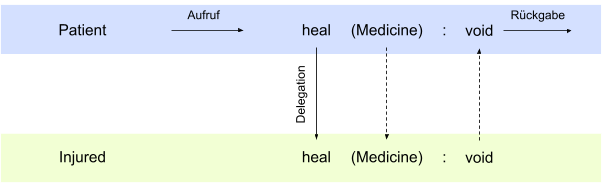
\includegraphics[width=\linewidth]{MDEL_heal}
\caption{Delegation der Methode $\texttt{heal}$}
\label{fig:DEL_heal}
\end{figure}
\noindent
An diesem Beispiel sind sowohl die Parameter- als auch die Rückgabe-Typen der aufgerufenen Methode und der Delegationsmethode identisch sind. Weiterhin spielt die Reihenfolge der Parameter in diesem Beispiel keine Rolle, da es nur einen Parameter gibt. Daher stellt die Übergabe der Parameter- und Rückgabewerte kein Problem dar.\\\\
Folgendes Beispiel soll zeigen, wie mit unterschiedlichen Reihenfolgen bzgl. der Parameter bei einer Methoden-Delegation umzugehen ist.
\paragraph{Beispiel} Die Methoden-Delegation aus Listing \ref{lst:methdel2} ist ein Beispiel für einen solchen Fall. Hier wird die aufgerufene Methode $\texttt{heal}$ mit den Parametern $\texttt{Patient}$ und $\texttt{MedCabinet}$ aus dem Typ $\texttt{PatientMedicalFireFighter}$ an die gleichnamige Methode aus dem Typ $\texttt{InverseDoctor}$ delegiert. Die Delegationsmethoden verwendet zwar identische Parameter-Typen, aber die Reihenfolge, in der die Parameter übergeben werden, ist unterschiedlich.
\begin{lstlisting}[style = dsl, caption = Methoden-Delegation mit Parametern in unterschiedlicher Reihenfolge, captionpos = b]
	PatientMedicalFireFighter.heal(Patient, MedCabinet):void --> posModi(1,0)  InverseDoctor.heal(MedCabinet,Patient):void
\end{lstlisting}\label{lst:methdel2}
\noindent
Um die Reihenfolge der Parameter aus dem ursprünglichen Aufruf zu variieren, wird das Schlüsselwort $\texttt{posModi}$ verwendet. Dort werden eine Reihe von Indizes angegeben. Die Anzahl der angegebenen Indizes muss mit der Anzahl der Parameter übereinstimmen. Ein Index beschreibt die Position des in der aufgerufenen Methode angegebenen Parameter. Weiterhin spielt die Reihenfolge der Indizes eine wichtige Rolle. Diese ist mit der Reihenfolge der Parameter der Delegationsmethoden gleichzusetzen.\\\\
So wird in dem o.g. Beispiel der erste Parameter der aufgerufenen Methoden (Index = 0) der Delegationsmethode als zweiter Parameter übergeben. Dementsprechende wird er zweite Parameter der aufgerufenen Methoden (Index = 1) der Delegationsmethode als erster Parameter übergeben (siehe Abbildung \ref{fig:DEL_healInverse}). 
\begin{figure}[H]
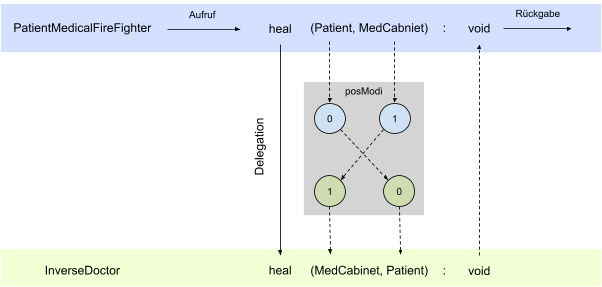
\includegraphics[width=\linewidth]{MDEL_healInverse}
\caption{Delegation der Methode $\texttt{heal}$ mit Parametern in unterschiedlicher Reihenfolge}
\label{fig:DEL_healInverse}
\end{figure}
\noindent
Ein weiteres Beispiel soll zeigen, wie mit übergebenen Typen umzugehen ist, die nicht ohne Probleme übergeben werden können. Dafür ist jedoch vorab zu klären, wann dies der Fall ist.\\\\
Dass identische Typen keine Probleme bei der Übergabe zwischen aufgerufener Methode und Delegationsmethode darstellen, wurde in den oben genannten Beispielen gezeigt.\\\\
Darüber hinaus können Typen aber auch dann ohne Probleme übergeben werden, wenn sie sich aufgrund des Substitutionsprinzips austauschen lassen. Daher kann ein Typ $T$ anstelle eines Typs $T'$ verwendet werden, sofern $T \leq T'$ gilt.
\paragraph{Beispiel} In folgendem Listing ist eine Methoden-Delegation aufgerührt, bei der sowohl die Parameter- als auch die Rückgabe-Typen der aufgerufenen Methode und der Delegationsmethode nicht auf Basis des Substitionsprinzips übergeben werden können.
\begin{lstlisting}[style = dsl, caption = Methoden-Delegation mit Typkonvertierung, captionpos = b]
	MedicalFireFighter.extinguishFire(ExtFire):boolean --> FireFigher.extinguishFire(Fire):FireState
\end{lstlisting}\label{lst:methdel3}
\noindent
In einem solchen Fall müssen die Parameter-Typen der aufgerufenen Methoden in die Parameter-Typen der Delegationsmethode konvertiert werden. Analog dazu muss der Rückgabetyp der Delegationsmethode in den Rückgabetyp der aufgerufenen Methoden konvertiert werden.\\\\
Angenommen, die Funktion $\mathit{proxies(S,T)}$ beschreibt eine Menge von Proxies, mit $S$ als Source-Typ und $T$ als Menge der Target-Typen. Dann müssten bezogen auf die Methoden-Delegation aus Listing 4 für die Parameter-Typen einer der Proxies aus der Menge $\mathit{proxies(\texttt{Fire}, \{\texttt{ExtFire}\})}$ an die Delegationsmethode übergeben werden. Nach der Ausführung der Delegationsmethode müsste ein Proxy aus der Menge $\mathit{proxies(\texttt{boolean},\{\texttt{FireState}\})}$ an die aufgerufenen Methode als Rückgabetyp übergeben werden. Der Sachverhalt wird in Abbildung \ref{fig:DEL_extinguishFire} schematisch dargestellt.
\begin{figure}[H]
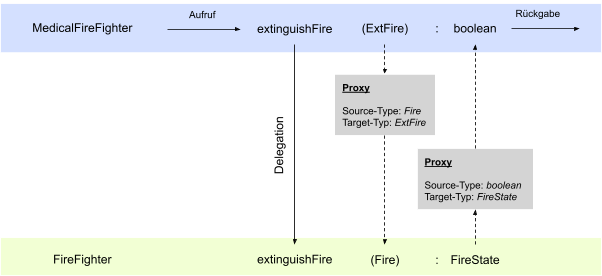
\includegraphics[width=\linewidth]{MDEL_extinguishFire}
\caption{Delegation der Methode $\texttt{extinguishFire}$ mit Typkonvertierungen}
\label{fig:DEL_extinguishFire}
\end{figure}
\noindent
Wie die Proxies generiert werden, wird im folgenden Abschnitt beschrieben.

\subsection{Generierung von Proxies}
Wie im Abschnitt \ref{sec:proxygram} bereits erwähnt, soll die Menge der Proxies für einen Source-Typ $S$ und einer Menge von Target-Typen $T$ über die Funktion $\mathit{proxies(S,T)}$ beschrieben werden.\\\\
In Abhängigkeit von dem Matching zwischen dem Source-Typ und den Target-Typen werden unterschiedliche Arten von Proxies generiert. Für die unterschiedlichen Proxy-Arten gibt es ebenfalls Funktionen, die eine Menge von Proxies zu einem Source-Typen $S$ und einer Menge von Target-Typen $T$ beschreiben.\\\\
In den folgenden Abschnitten werden diese Funktionen für die einzelnen Proxy-Arten beschrieben. Dabei ist davon auszugehen, dass die Proxies eine allgemeine Struktur haben, die in Abschnitt \ref{sec:proxygram} aufgeführt ist. Um die Regeln für die Generierung der Proxies zu beschreiben, soll davon ausgegangen werden, dass jedes Listen-Attribut ($\mathit{NT.}\text{*}$) aus Tabelle \ref{tab:attrGrProxies} ein Attribut $\texttt{len}$ enthält in dem die Anzahl der in der Liste befindlichen Elemente abgelegt ist.


\subsubsection{Sub-Proxy}
Die Voraussetzung für die Erzeugung eines \emph{Sub-Proxies} vom Typ $T$ aus einem Target-Typ $T'$ ist $T \Rightarrow_{spec} T'$. Damit ist der \emph{SpecTypeMatcher} der Basis-Matcher für den Sub-Proxy.
\paragraph{Beispiel}
Als Beispiel soll  der Typ $\texttt{Patient}$ als Source-Typ und der Typ $\texttt{Injured}$ als Target-Typ verwendet werden. Da $\texttt{Patient} \Rightarrow_{spec} \texttt{Injured}$ gilt, kann ein \emph{Sub-Proxy} für diese Konstellation erzeugt werden. Der resultierende \emph{Sub-Proxy} ist im folgenden Listing aufgeführt.
\begin{lstlisting}[style = dsl, caption = Sub-Proxy für Patient, captionpos = b]
proxy for Patient with [Injured]{
	Patient.heal(Medicine):void --> Injured.heal(Medicine):void
	Patient.getName():String --> err
}
\end{lstlisting}
Der abstrakte Syntaxbaum mit den dazugehörigen Attributen ist Abbildung \ref{fig:ASTSUB} zu entnehmen. \footnote{Es wurden nur die Nonterminale mit den dazugehörigen Attributen aufgeführt.}
\begin{figure}[h!]
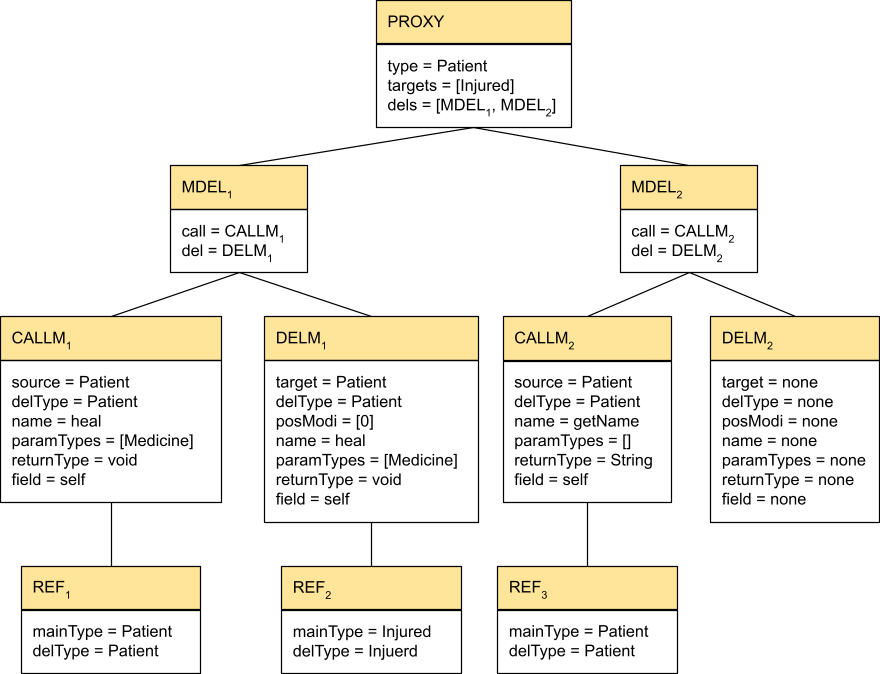
\includegraphics[width=\linewidth]{AST_SubExample}
\caption{AST für das Beispiel zum Sub-Proxy}
\label{fig:ASTSUB}
\end{figure}
\noindent
Der Proxy bietet alle Methoden an, die auch von dessen Source-Typ angeboten werden. Die Methodendelegationen innerhalb des Proxies, beschreiben, was beim Aufruf der jeweiligen aufgerufenen Methoden passiert. So wird ein Aufruf der Methode $\texttt{heal}$ an die Methode $\texttt{heal}$ aus dem Target-Typ delegiert. Ein Aufruf der Methode $\texttt{getName}$ hingegen führt zu einem Fehler, weil keine Delegationsmethode zur Verfügung steht.\\\\
Im Hinblick darauf, dass eine Konvertierung von einem Super-Typ und einen Sub-Typ (Down-Cast) ebenfalls dazu führt, dass bestimmte Methoden, wie in diesem Fall $\texttt{getName}$ nicht ausgeführt werden können, spiegelt der \emph{Sub-Proxy} dieses Verhalten wieder.
\paragraph{Formalisierung}
Formal wird ein \emph{Sub-Proxy} durch die Regeln beschrieben, die im Folgenden vorgestellt werden. Ein \emph{Sub-Proxy} enthält genau einen Target-Typ. Für einen Proxy $P$ wird dieser Sachverhalt durch die folgende Regel dargestellt.
\begin{gather*}
\frac{|\mathit{P.targets}| = 1 \wedge \forall \mathit{T'} \in \mathit{P.targets}: T = T'}{\mathit{targets_{single}(P,T)}}
\end{gather*}
Darüber hinaus enthält ein \emph{Sub-Proxy} $P$ eine bestimmte Menge von Methoden-Delegationen. Dabei muss in allen Methodendelegationen das Attribut $\texttt{field}$ der aufgerufenen Methoden mit dem der Delegationsmethoden übereinstimmen. Folgende Regel stellt diesen Sachverhalt für eine Menge von Methoden-Delegationen $\mathit{MDList}$ dar.
\begin{gather*}
\frac{\splitfrac{\forall \mathit{MD_1}\in \mathit{MDList}: \neg(\exists \mathit{MD_2} \in \mathit{MDList}:\mathit{MD_1.call.field} \neq \mathit{MD_2.call.field}}{ \vee \mathit{MD_1.del.field} \neq \mathit{MD_2.del.field} )}}
{\mathit{equalRefs(MDList)}}
\end{gather*}
Für jede einzelne Methoden-Delegation $\mathit{MD}$ gilt weiterhin, dass die aufgerufene Methode und die Delegationsmethode denselben Namen haben.
\begin{gather*}
\frac{\mathit{MD.call.name} = \mathit{MD.del.name}}
{\mathit{methDel_{nominal}(MD)}}
\end{gather*}
Die aufgerufene Methode muss dabei generell im Typ aus dem Attribut $\texttt{call.delType}$ deklariert sein und die Delegationsmethode im Typ aus dem Attribut $\texttt{del.delType}$.
\begin{gather*}
\frac{\exists \mathit{T'\text{ } m(T)} \in \mathit{methoden(MD.call.delType)}: \mathit{MD.call.name} = m}
{\mathit{callMethod_{simple}(MD)}}
\end{gather*}
\begin{gather*}
\frac{\exists \mathit{T'\text{ }m(T)} \in \mathit{methoden(MD.del.delType)}: \mathit{MD.del.name} = m}
{\mathit{delMethod_{simple}(MD)}}
\end{gather*}
Zusätzlich muss das Attribut $\texttt{field}$ im Attribut $\texttt{call}$ mit dem Wert $\texttt{self}$ belegt und das Attribut $\texttt{mainType}$ mit dem Source-Typ des Proxies belegt sein.
\begin{gather*}
\frac{\mathit{MD.call.mainType} = \mathit{P.type} \wedge \mathit{MD.call.field} = \mathit{self}}
{\mathit{callMethodDelType_{simple}(MD, P)}}
\end{gather*}
Damit ist auch automatisch gewährleistet, dass die Attribute $\texttt{mainType}$ und $\texttt{delType}$ im Attribut $\texttt{call}$ übereinstimmen. (siehe Tabelle \ref{tab:attrGrProxies})\\\\
Ähnliches gilt für die Attribute $\texttt{field}$ und $\texttt{mainType}$ im Attribut $\texttt{del}$. Hierbei muss der Wert des Attributs $\texttt{mainType}$ jedoch mit dem Target-Typ des Proxies übereinstimmen.
\begin{gather*}
\frac{\mathit{MD.del.field} = \mathit{self} \wedge  \mathit{MD.del.mainType} \in \mathit{P.targets} }
{\mathit{delMethodDelType_{simple}(MD, P)}}
\end{gather*}
Damit ist wiederum automatisch gewährleistet, dass die Attribute $\texttt{mainType}$ und $\texttt{delType}$ im Attribut $\texttt{del}$ übereinstimmen. (siehe Tabelle \ref{tab:attrGrProxies})\\\\
Die Regeln für die linke Seite einer Methoden-Delegation $\mathit{MD}$ innerhalb eines \emph{Sub-Proxies} $P$ können damit in folgender Regel zusammengefasst werden:
\begin{gather*}
\frac{\mathit{callMethod_{simple}(MD)} \wedge \mathit{callMethodDelType_{simple}(MD,P)}}
{\mathit{call_{simple}(MD,P)}}
\end{gather*}
Analog dazu können auch die Regeln für die rechte Seite einer Methoden-Delegation $\mathit{MD}$ innerhalb eines \emph{Sub-Proxies} $P$ zusammengefasst werden:
\begin{gather*}
\frac{\mathit{delMethod_{simple}(MD)} \wedge \mathit{delMethodDelType_{simple}(MD,P)}}
{\mathit{del_{simple}(MD,P)}}
\end{gather*}
Im \emph{Sub-Proxy} ist darüber hinaus noch die Methoden-Delegation zu beachten, die bei einem Aufruf zu einem Fehler führt. Dieser Fall wird für eine Methoden-Delegation $\mathit{MD}$ wie folgt beschrieben:
\begin{gather*}
\frac{\mathit{MD.del.name} = \mathit{none}}
{\mathit{del_{err}(MD)}}
\end{gather*}
Die genannten Regeln für eine Methoden-Delegation $\mathit{MD}$ in einem \emph{Sub-Proxy} lassen sich über die beiden folgenden Regeln beschreiben:
\begin{gather*}
\frac{\mathit{call_{simple}(MD,P)} \wedge \mathit{del_{simple}(MD,P) \wedge \mathit{methDel_{nominal}(MD)}}}
{\mathit{methDel_{sub}(MD,P)}}
\end{gather*}
\begin{gather*}
\frac{\mathit{call_{simple}(MD,P)}\wedge\mathit{del_{err}(MD)}
}
{\mathit{methDel_{sub}(MD,P)}}
\end{gather*}
Innerhalb eines \emph{Sub-Proxies} gibt es für jede Methode $m$ des Source-Typ genau eine Methoden-Delegation mit der Methode $m$ als aufgerufene Methode. Damit lässt sich für einen Proxy $P$ in Bezug auf alle seine Methoden-Delegationen folgende Regeln formulieren:
\begin{gather*}
\frac{\splitfrac{\mathit{M} = \mathit{methoden(P.type)}\wedge|\mathit{M}| = |P.dels| \wedge \forall \mathit{T'\text{ }m(T)} \in \mathit{M}:}{\exists \mathit{MD} \in \mathit{P.dels}:m = \mathit{MD.call.name} \wedge \mathit{methDel_{sub}(MD,P)
 }}
}
{\mathit{methDelList_{sub}(P)}}
\end{gather*}
Für einen Proxy $P$ kann die Regel $\mathit{equalRefs(P)}$ im Allgemeinen mit der Bedingung zusammengefasst werden, die besagt, dass ein Proxy immer einen bestimmten Source-Typ $S$ haben muss. Die zusammengefasste Regel lautet:
\begin{gather*}
\frac{\mathit{P.type} = \mathit{S} \wedge \mathit{equalRefs(P)}}{\mathit{proxy(P,S)}}
\end{gather*}
\noindent
Die Menge der \emph{Sub-Proxies}, die mit dem Source-Typ $T$ und dem Target-Typ $T'$ erzeugt werden, wird durch die folgende Funktion beschrieben.
\begin{gather*}
\mathit{proxies_{sub}(T,T')} := 
\left\{\begin{array}{l|l}
		& \mathit{proxy(P,T)}\wedge \mathit{ } \\
	P	& \mathit{targets_{single}(P,T')} \wedge \mathit{ } \\
		& \mathit{methDelList_{sub}(P)}
		 \end{array}
\right\}
\end{gather*}


\subsubsection{Content-Proxy}
Die Voraussetzung für die Erzeugung eines \emph{Content-Proxies} vom Typ $T$ aus einem Target-Typ $T'$ ist $T \Rightarrow_{content} T'$. Damit ist der \emph{ContentTypeMatcher} der Basis-Matcher für den \emph{Content-Proxy}.
\paragraph{Beispiel} Als Beispiel sollen die Typen $\texttt{Medicine}$ und $\texttt{MedCabinet}$ verwendet werden, welche ein Matching der Form $\texttt{Medicine} \Rightarrow_{content} \texttt{MedCabinet}$ aufweisen. Daher kann ein \emph{Content-Proxy} für diese Konstellation erzeugt werden. Ein resultierender \emph{Content-Proxy} ist in folgendem Listing aufgeführt.
\begin{lstlisting}[style = dsl, caption = Content-Proxy für Medicine, captionpos = b]
proxy for Medicine with [MedCabinet]{
	Medicine.getDesciption():String --> MedCabinet.med.getDesciption():String
}
\end{lstlisting}
Durch die Methoden-Delegation dieses \emph{Content-Proxies} wird die Methode $\texttt{getDescription}$ an das Feld $\texttt{med}$ des Target-Typen $\texttt{MedCabniet}$ delegiert.\\\\
Der abstrakte Syntaxbaum mit den dazugehörigen Attributen ist Abbildung \ref{fig:ASTCONTENT} zu entnehmen. \footnote{Es wurden nur die Nonterminale mit den dazugehörigen Attributen aufgeführt.}
\begin{figure}[h!]
\centering
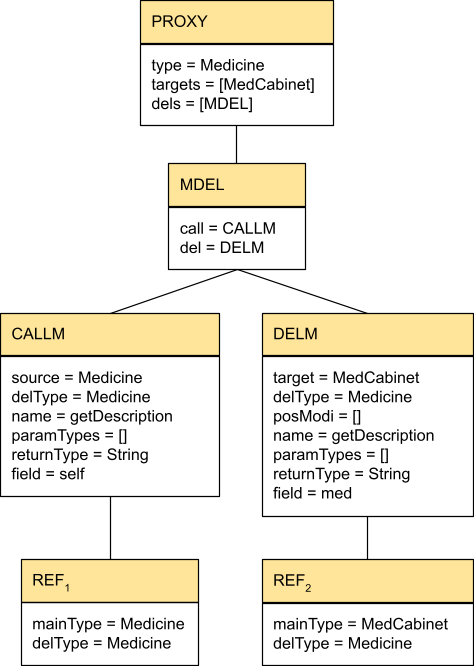
\includegraphics[width=0.5\linewidth]{AST_ContentExample}
\caption{AST für das Beispiel zum Content-Proxy}
\label{fig:ASTCONTENT}
\end{figure}
\noindent
\paragraph{Formalisierung}
Formal wird ein \emph{Content-Proxy} durch die Regeln beschrieben, die im Folgenden vorgestellt werden.\\\\
Ein \emph{Content-Proxy} enthält, wie auch der \emph{Sub-Proxy}, genau einen Target-Typ. Ebenfalls identisch zum \emph{Sub-Proxy} sind die Bedingungen hinsichtlich der aufgerufenen Methoden in den einzelnen Methoden-Delegationen.\\\\
In den Delegationsmethoden einer einzelnen Methoden-Delegation $\mathit{MD}$ dürfen die Attribute $\texttt{mainType}$ und $\texttt{delType}$ im \emph{Content-Proxy} nicht identisch sein. Dementsprechend darf das Attribut $\texttt{field}$ nicht mit dem Wert $\texttt{self}$ belegt sein. Vielmehr muss für das Attribut $\texttt{delTyp}$ und den Source-Typ $T$ des Proxies ein Matching der Form $T \Rightarrow_{internCont} \mathit{MD.del.delTyp}$ gelten. Daher gilt für den \emph{Content-Proxy} die folgende Regel:
\begin{gather*}
\frac{\mathit{P.type} \Rightarrow_{internCont} \mathit{MD.del.delType}  \wedge \mathit{MD.del.mainType} \in \mathit{P.targets}}
{\mathit{delMethodDelType_{content}(MD,P)}}
\end{gather*}
\noindent
Damit kann eine zusammenfassende Regel für die Delegationsmethoden einer Methoden-Delegation $\mathit{MD}$ wie folgt definiert werden:
\begin{gather*}
\frac{\mathit{delMethod_{simple}(MD)} \wedge \mathit{delMethodDelType_{content}(MD,P)}}
{\mathit{del_{content}(MD,P)}}
\end{gather*}
Die zusammenfassende Regel für eine einzelne Methoden-Delegation $\mathit{MD}$ innerhalb eines \emph{Content-Proxies} hat die folgende Form:
\begin{gather*}
\frac{\mathit{call_{simple}(MD,P)} \wedge \mathit{del_{content}(MD,P) \wedge \mathit{methDel_{nominal}(MD)}}}
{\mathit{methDel_{content}(MD,P)}}
\end{gather*}
Wie auch im \emph{Sub-Proxy} gibt es im \emph{Content-Proxy} für jede Methode $m$ des Source-Typen genau eine Methoden-Delegation mit der Methode $m$ als aufgerufene Methode. Daraus ergibt sich für alle Methoden-Delegationen aus einem \emph{Content-Proxy} $P$ folgende Regel:
\begin{gather*}
\frac{\splitfrac{M = \mathit{methoden(P.type) }\wedge|\mathit{M}| = |\mathit{P.dels}| \wedge \forall \mathit{T' \text{ }m(T)} \in \mathit{M}:}{ \exists \mathit{MD} \in \mathit{P.dels}:m = \mathit{MD.call.name} \wedge \mathit{methDel_{content}(MD,P)
 }
}}
{methDelList_{content}(P)}
\end{gather*}
Die Menge der \emph{Content-Proxies}, die mit dem Source-Typ $T$ und dem Target-Typ $T'$ erzeugt werden, wird durch die folgende Funktion beschrieben.
\begin{gather*}
\mathit{proxies_{content}(T,T')} := 
\left\{\begin{array}{l|l}
		& \mathit{proxy(P,T)} \wedge \mathit{ } \\
	P	& \mathit{targets_{single}(P,T')} \wedge \mathit{ }\\
		& \mathit{methDelList_{content}(P)} 
		 \end{array}
\right\}
\end{gather*}
\subsubsection{Container-Proxy}
Die Voraussetzung für die Erzeugung eines \emph{Container-Proxies} vom Typ $T$ aus einem Target-Typ $T'$ ist $T \Rightarrow_{container} T'$. Damit ist der \emph{ContainerTypeMatcher} der Basis-Matcher für den \emph{Container-Proxy}.
\paragraph{Beispiel}
Als Beispiel werden wiederum die Typen $\texttt{Medicine}$ und $\texttt{MedCabinet}$ verwendet, welche ein Matching der Form $\texttt{MedCabinet} \Rightarrow_{container} \texttt{Medicine}$ aufweisen. Daher kann ein \emph{Content-Proxy} für diese Konstellation erzeugt werden. Ein resultierender \emph{Content-Proxy} ist in folgendem Listing aufgeführt.
\begin{lstlisting}[style = dsl, caption = Container-Proxy für MedCabniet, captionpos = b ]
proxy for MedCabinet with [Medicine]{
	MedCabinet.med.getDesciption():String --> Medicine.getDesciption():String
}
\end{lstlisting}
Durch die Methoden-Delegation dieses \emph{Container-Proxies} findet eine Delegation nur dann statt, wenn die Methoden $\texttt{getDescription}$ auf dem Feld $\texttt{med}$ des Source-Typ aufgerufen wird. Diese wird dann an den Target-Typen $\texttt{MedCabniet}$ delegiert.\\\\
Der abstrakte Syntaxbaum mit den dazugehörigen Attributen ist Abbildung \ref{fig:ASTCONTAINER} zu entnehmen. \footnote{Es wurden nur die Nonterminale mit den dazugehörigen Attributen aufgeführt.}
\begin{figure}[h!]
\centering
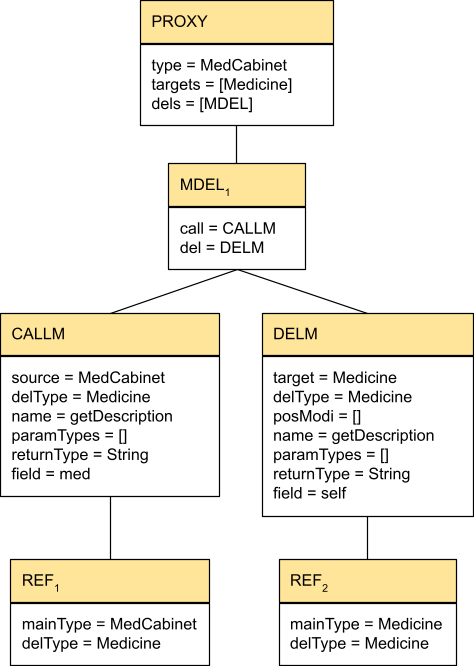
\includegraphics[width=0.5\linewidth]{AST_ContainerExample}
\caption{AST für das Beispiel zum Container-Proxy}
\label{fig:ASTCONTAINER}
\end{figure}
\noindent
\paragraph{Formalisierung}
Formal wird ein \emph{Container-Proxy} durch die Regeln beschrieben, die im Folgenden vorgestellt werden.\\\\
Ein \emph{Container-Proxy} enthält, wie die vorher beschriebenen Proxies, genau einen Target-Typ. Die Eigenschaften der Delegationsmethoden innerhalb der einzelnen Methoden-Delegationen gleichen denen aus dem \emph{Sub-Proxy}.\\\\
In den angerufenen Methoden einer einzelnen Methoden-Delegation $\mathit{MD}$ dürfen die Attribute $\texttt{mainType}$ und $\texttt{delType}$ im \emph{Container-Proxy} nicht übereinstimmen. Dementsprechend darf das Attribut $\texttt{field}$ nicht mit dem Wert $\texttt{self}$ belegt sein. Vielmehr müssen der Wert des Attributs $\texttt{delTyp}$ und der Target-Typ $T$ des Proxies ein Matching der Form $T \Rightarrow_{internCont} \texttt{delTyp}$ ausweisen. Daher gilt für den \emph{Container-Proxy} $P$ folgende Regel.
\begin{gather*}
\frac{\splitfrac{\mathit{MD.call.mainType} = \mathit{P.type} \wedge \forall \mathit{T} \in \mathit{P.targets}:}
{  \mathit{T} \Rightarrow_{internCont} \mathit{MD.call.delType}}
}
{\mathit{callMethodDelType_{container}(MD,P)}}
\end{gather*}
\noindent
Damit kann eine zusammenfassende Regel für die aufgerufenen Methoden wie folgt definiert werden:
\begin{gather*}
\frac{\mathit{callMethod_{simple}(MD)} \wedge \mathit{callMethodDelType_{container}(MD,P)}}
{\mathit{call_{container}(MD,P)}}
\end{gather*}
Die zusammenfassende Regel für eine einzelne Methoden-Delegation $\mathit{MD}$ innerhalb eines \emph{Container-Proxies} hat die folgende Form:
\begin{gather*}
\frac{\mathit{call_{container}(MD,P)} \wedge \mathit{del_{simple}(MD,P)} \wedge \mathit{methDel_{nominal}(MD)}}
{\mathit{methDel_{container}(MD,P)}}
\end{gather*}
Für einen \emph{Container-Proxy} $P$ gilt ebenfalls die Regel $\mathit{equalRefs(P.dels)}$. Daher müssen die Werte des Attributs $\texttt{call.delType}$ aller Methoden-Delegationen des Proxies $P$ übereinstimmen. Ferner muss es für jede Methode $m$ des Typen aus $\texttt{call.delType}$ genau eine Methoden-Delegation mit der Methode $m$ als aufgerufene Methode existieren. Daraus ergibt sich für alle Methoden-Delegationen aus einem \emph{Content-Proxy} $P$ folgende Regel:
\begin{gather*}
\frac{\splitfrac{\mathit{M} = \mathit{methoden(P.dels[0].call.delType)} \wedge |\mathit{M}| = |P.dels| \wedge \forall \mathit{T' \text{ } m(T)} \in \mathit{M}:}
{\exists \mathit{MD} \in P.dels:m = \mathit{MD.call.name} \wedge \mathit{methDel_{container}(MD,P)}
 }}
{\mathit{methDelList_{container}(P)}}
\end{gather*}
Die Menge der \emph{Container-Proxies}, die mit dem Source-Typ $T$ und dem Target-Typ $T'$ erzeugt werden, wird durch die folgende Funktion beschrieben.
\begin{gather*}
\mathit{proxies_{container}(T,T')} := 
\left\{\begin{array}{l|l}
		& \mathit{proxy(P,T)}  \wedge \mathit{ } \\
	P	& \mathit{target_{single}(P,T')} \wedge \mathit{ } \\
		& \mathit{methDelList_{container}(P)} 
		 \end{array}
\right\}
\end{gather*}

\subsubsection{Struktureller Proxy}
Die Voraussetzung für die Erzeugung eines \emph{strukturellen Proxies} vom \emph{required Typ} $R$ aus einem Target-Typ $T$ ist $R \Rightarrow_{struct} T$. Damit ist der \emph{StructuralTypeMatcher} der Basis-Matcher für den \emph{strukturellen Proxy}.\\\\
Der \emph{strukturelle Proxy} ist der einzige Proxy, der mit mehreren Target-Typen erzeugt werden kann. 
\paragraph{Beispiel}
Als Beispiel werden die Typen $\texttt{MedicalFireFighter}$, $\texttt{Doctor}$ und $\texttt{FireFighter}$ verwendet. Dabei ist $\texttt{MedicalFireFighter}$ der Source-Typ des Proxies und die Menge der anderen beiden Typen bilden die Target-Typen des Proxies. Da der Source-Typ zu den Target-Typen ein Matching der Form $\texttt{MedicalFireFighter} \Rightarrow_{struct} \texttt{FireFighter}$ bzw. $\texttt{MedicalFireFighter} \Rightarrow_{struct} \texttt{Doctor}$ aufweist, kann ein \emph{struktureller Proxy} erzeugt werden. Ein solcher ist in folgendem Listing aufgeführt.
\begin{lstlisting}[style = dsl, caption = Struktureller Proxy für MedicalFireFighter, captionpos = b]
proxy for MedicalFireFighter with [Doctor, FireFighter]{
	MedicalFireFighter.heal(Patient, MedCabinet):void --> Doctor.heal(Patient, Medicine):void
	MedicalFireFighter.extinguishFire(ExtFire):boolean --> FireFighter.extinguishFire(Fire):FireState
}
\end{lstlisting}
In diesem Beispiel wird der Methodenaufruf der Methode $\texttt{heal}$ auf dem Proxy an die Methode $heal$ des Typs $\texttt{Doctor}$ delegiert. Analog dazu würde ein Aufruf der Methode $\texttt{extinguishFire}$ auf dem Proxy an die Methode $extinguishFire$ des Typs $\texttt{FireFighter}$ delegiert werden. Die Methoden stimmen jeweils strukturell überein.\\\\
Der abstrakte Syntaxbaum mit den dazugehörigen Attributen ist Abbildung \ref{fig:ASTSTRUCT} zu entnehmen. \footnote{Es wurden nur die Nonterminale mit den dazugehörigen Attributen aufgeführt.}
\begin{figure}[h!]
\centering
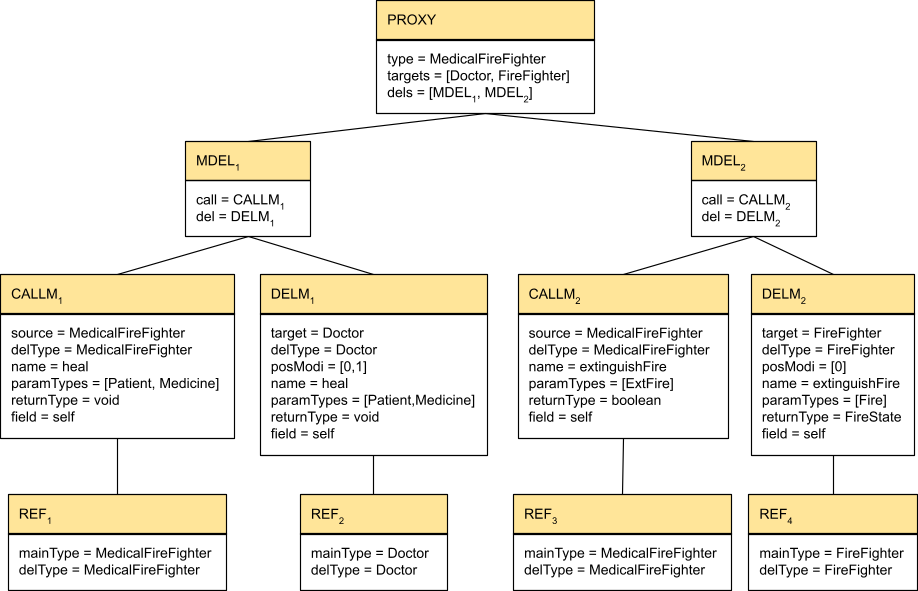
\includegraphics[width=\linewidth]{AST_StructExample}
\caption{AST für das Beispiel zum strukturellen Proxy}
\label{fig:ASTSTRUCT}
\end{figure}
\noindent
\paragraph{Formalisierung}
Ein \emph{struktureller Proxy} wird formal durch die folgenden Regeln beschrieben.\\\\
Ein \emph{struktureller Proxy} kann, wie bereits erwähnt, mehrere Target-Typen enthalten.
Für jeden Target-Typ $T$ muss dabei jedoch wenigstens eine Delegationsmethode im Proxy mit einem Attribut $\texttt{target} = T$ existiert. Dadurch gilt die für einen \emph{strukturellen Proxy} Proxy $P$:
\begin{gather*}
\frac{\forall \mathit{T} \in \mathit{P.targets}:\exists \mathit{MD} \in \mathtt{P.dels}:\mathit{MD.del.target} = T}{\mathit{targets_{struct}(P, T)}}
\end{gather*}
Für die aufgerufene Methode und die Delegationsmethode einer einzelnen Methoden-Delegation $\mathit{M}$ gelten im \emph{strukturellen Proxy} dieselben Regeln wie für den \emph{Sub-Proxy}. Die Namen der aufgerufenen Methode und der Delegationsmethode müssen dabei jedoch nicht übereinstimmen. Dafür müssen diese beiden Methode jedoch ein strukturelles Matching aufweisen. Bezogen auf die Rückgabe-Typen einer aufgerufenen Methode $\mathit{C}$ und der Delegationsmethode $\mathit{D}$ aus einer Methoden-Delegation muss daher Folgendes gelten.
\begin{gather*}
\frac{\mathit{D.returnType} \Rightarrow_{internStruct} \mathit{C.returnType}}{\mathit{return_{struct}(C,D)}}
\end{gather*} 
Weiterhin muss für die Parameter-Typen gelten:
\begin{gather*}
\frac{\mathit{C.paramCount} = 0}{\mathit{params_{struct}(C,D)}}
\end{gather*} 
\begin{gather*}
\frac{\splitfrac{\forall \mathit{i} \in \{0,...,\mathit{C.paramCount}-1\}:}
{ \mathit{C.paramTypes}[i] \Rightarrow_{internStruct} \mathit{D.paramTypes}[\mathit{D.posModi}[i]]
}}{\mathit{params_{struct}(C,D)}}
\end{gather*} 
Für eine einzelne Methoden-Delegation $\mathit{MD}$ eines \emph{strukturellen Proxies} $P$ kann dann folgende Regel aufgestellt werden.
\begin{gather*}
\frac{\splitfrac{\mathit{call_{simple}(MD,P)} \wedge \mathit{del_{simple}(MD,P)} \wedge} {\mathit{return_{struct}(MD.call, MD.del)} \wedge \mathit{params_{struct}(MD.call, MD.del)}}
}
{\mathit{methDel_{struct}(MD,P)}}
\end{gather*}
In einem \emph{strukturellen Proxy} muss für jede Methode $m$ des Source-Typen genau eine Methoden-Delegation mit der Methode $m$ als aufgerufene Methode existieren. Daraus ergibt sich für alle Methoden-Delegationen aus einem \emph{strukturellen Proxy} $P$ folgende Regel:
\begin{gather*}
\frac{\splitfrac{\mathit{M} = \mathit{methoden(P.type)} \wedge |\mathit{M}| = |\mathit{P.dels}| \wedge \forall \mathit{T' \text{ }m(T)} \in \mathit{M}:}{\exists \mathit{MD} \in \mathit{P.dels}:\mathit{MD.call.name} = m \wedge \mathit{methDel_{struct}(MD,P)}
 }
}
{\mathit{methDelList_{struct}(P)}}
\end{gather*}
Wie in Abschnitt 
Die Menge der \emph{strukturellen Proxies}, die mit dem Source-Typ $R$ und der Menge von Target-Typen $T$ erzeugt werden, wird durch die folgende Funktion beschrieben.
\begin{gather*}
\mathit{proxies_{struct}(R,T)} := 
\left\{\begin{array}{l|l}
		& \mathit{proxy(P,R)}\wedge \mathit{ }\\
	P	& \mathit{targets_{struct}(P,T)} \wedge \mathit{ }\\
		& \mathit{methDelList_{struct}(P)}  
		 \end{array}
\right\}
\end{gather*}

\paragraph{Allgemeine Generierung von Proxies}
Die Proxy-Funktion der einzelnen Proxy-Arten werden zur Beschreibung einer allgemeine Funktion für die Generierung der Proxies verwendet. Dazu sind die Proxy-Arten zusammen mit den dazugehörigen Matchingrelationen und Proxy-Fukntionen in Tabelle \ref{tab:baseMatcher} noch einmal aufgeführt.

\begin{table}[H]
\centering
\begin{tabular}{|c|c|c|}
\hline
\hline
\centering\textbf{Proxy-Art} & \textbf{Matchingrelation} & \textbf{Funktionsname}\\
\hline
\hline
Sub-Proxy
&  
$\Rightarrow_{spec}$
& 
$\mathit{proxies_{sub}}$
\\
\hline
Content-Proxy
& 
$\Rightarrow_{content}$
& 
$\mathit{proxies_{content}}$
\\
\hline
Container-Proxy
& 
$\Rightarrow_{container}$
& 
$\mathit{proxies_{container}}$
\\
\hline
struktureller Proxy
&
$\Rightarrow_{struct}$
& 
$\mathit{proxies_{struct}}$
 \\
\hline
\hline
\end{tabular}
\caption{Proxy-Arten mit Matchingrelationen und Proxy-Funktionen}
 \label{tab:baseMatcher}
\end{table}
\noindent
Die im Abschnitt \ref{sec:proxygram} erwähnte Funktion $\mathit{proxies(S,T)}$ kann darauf aufbauend für einen Source-Typ $S$ und eine Menge von Target-Typen $T$ wie folgt beschrieben werden.
\begin{gather*}
\mathit{proxies(S,T)} := 
\left\{\begin{array}{ll}
\mathit{proxy_{sub}(S,T)}	& \text{wenn } |T| = 1 \wedge \mathit{ }\\
& \forall T' \in T: S \Rightarrow_{sub} T'\\	
&\\
\mathit{proxy_{content}(S,T)}	& \text{wenn } |T| = 1 \wedge \mathit{ }\\
& \forall T' \in T: S \Rightarrow_{content} T' \\
&\\
\mathit{proxy_{container}(S,T)} & \text{wenn } |T| = 1 \wedge \mathit{ } \\
& \forall T' \in T: S \Rightarrow_{container} T' \\
&\\
\mathit{proxy_{struct}(S,T)} & \text{wenn } |T| > 0 \wedge \mathit{ } \\
&\forall T' \in T: S \Rightarrow_{struct} T'
		 \end{array}
\right\}
\end{gather*}
\subsection{Anzahl möglicher Proxies innerhalb einer Bibliothek}
Die Generierung der Proxies für ein required Typ $R$ aus der Bibliothek $L$ erfolgt während der Exploration mit den Mengen von provided Typen aus $\mathit{cover(R,L)}$ (siehe Abschnitt \ref{sec_ergStructEval}). Mit einer Menge $T \in \mathit{cover(R,L)}$ können durchaus mehrere Proxies erzeugt werden. Das ist dann der Fall, wenn mehrere der Methoden, die in den provided Typen aus $T$ deklariert wurden, mit einer Methode des required Typs $R$ strukturell übereinstimmen.
Die Anzahl der möglichen Proxies für ein required Typ $R$ mit einer bestimmten Mengen von Target-Typen $T_1,...,T_k$ ist somit von der Anzahl der Methoden abhängig, die in einem der Target-Typen des Proxies deklariert wurden und strukturell mit den Methoden aus $R$ übereinstimmen. 
\\\\
Die Menge der Methoden eines provided Typen $P$, die strukturell mit einer Methode $m$ übereinstimmen, wird über die Funktion $\mathit{structM_{target}}$ beschrieben.
\begin{gather*}
\mathit{structM_{target}(m, P)} := 
\left\{\begin{array}{l|l}
m'	& m' \in \mathit{methoden(P)} \wedge  m \Rightarrow_{method} m'
\end{array}
\right\}
\end{gather*}
\noindent
Darauf aufbauend wird die Menge der Methoden einer Menge von \emph{provided Typen} $T$, die strukturell mit einer Methode $m$ übereinstimmen, über die Funktion $\mathit{structM_{targetset}}$ beschrieben.
\begin{gather*}
\mathit{structM_{targetset}(m, T)} := 
\left\{\begin{array}{l|l}
m'	& \exists P \in T: m' \in \mathit{structM_{target}(m,P)}
\end{array}
\right\}
\end{gather*}
\noindent
Sei $R$ ein \emph{required Typ} und $T$ eine Menge von \emph{provided Typen} innerhalb einer Bibliothek $L$ mit $T \in \mathit{cover(R,L)}$. Dann bildet die Funktion $\mathit{structMSets}$ die Mengen der Methoden aus den \emph{provided Typen} ab, die mit jeweils einer Methode aus $R$ gematcht werden können.
\begin{gather*}
\mathit{structMSets(R,T)} := 
\left\{M
\begin{array}{l|l}
&\exists \mathit{m} \in \mathit{methoden(R)} : 
\\
&M = \mathit{structM_{targetset}(m,T)}
\end{array}
\right\}
\end{gather*}
\noindent
%Dann bilden $M_1,...,M_n$ wie folgt die Mengen der Methoden der Target-Typen in $T$, die mit jeweils einer Methode $m_i \in \mathit{methoden(R)}$  strukturell übereinstimmen.
%\begin{gather*}
%M_1 = \mathit{structM_{target}(m_1,T)}\\
%...\\
%M_n = \mathit{structM_{target}(m_n,T)}
%\end{gather*}
Für jede Kombination von jeweils einem Element aus jeder der Mengen aus $\mathit{structMSets(R,T)}$ kann ein Proxy für $R$ mit der Menge der Target-Typen $T$ erzeugt werden.

\begin{example}{bsp_structmtarget}
Aufbauend auf dem vorherigen Beispiel \ref{bsp_cover} ergeben sich für die Menge der Target-Typen  $\{\texttt{Leave}, \texttt{Come}\}$ und die beiden Methoden des required Typs $\texttt{Greeting}$ folgende Menge von übereinstimmenden Methoden über die Funktion $\mathit{structMSets}$:
\begin{gather*}
\mathit{structMSets(\methodForm{String}{hello}{},\{\texttt{Leave}, \texttt{Come}\})} = 
\left\{
\begin{array}{l}
\methodForm{String}{hello}{},\\
\methodForm{String}{goodMorning}{},\\
\methodForm{String}{bye}{}
\end{array}
\right\}\\
\mathit{structMSets(\methodForm{String}{bye}{},\{\texttt{Leave}, \texttt{Come}\})} = 
\left\{
\begin{array}{l}
\methodForm{String}{hello}{},\\
\methodForm{String}{goodMorning}{},\\
\methodForm{String}{bye}{}
\end{array}
\right\}
\end{gather*}
\noindent
Darauf aufbauend lassen sich die folgenden vier Proxies mit den Target-Typen $\texttt{Leave}$ und $\texttt{Come}$ erzeugen.
\begin{lstlisting}[style = dsl]
proxy Greeting with [Come, Leave]{
	Greeting.hello():String --> Come.hello():String
	Greeting.bye():String --> Leave.bye():String
}
\end{lstlisting}
\begin{lstlisting}[style = dsl]
proxy Greeting with [Come, Leave]{
	Greeting.hello():String --> Come.goodMorning():String
	Greeting.bye():String --> Leave.bye():String
}
\end{lstlisting}
\begin{lstlisting}[style = dsl]
proxy Greeting with [Come, Leave]{
	Greeting.hello():String --> Leave.bye():String
	Greeting.bye():String --> Come.hello():String
}
\end{lstlisting}
\begin{lstlisting}[style = dsl]
proxy Greeting with [Come, Leave]{
	Greeting.hello():String --> Leave.bye():String
	Greeting.bye():String --> Come.goodMorning():String
}
\end{lstlisting}
\end{example}
\noindent
Für die Bildung eines Proxies wird aus jeder der oben genannten Menge $\{M_1,...,M_n\} = structMSets(R,T)$ genau ein Element als Delegationsmethode verwendet werden. Die Anzahl aller möglichen Proxies für ein \emph{required Typ} $R$ aus einer Menge von Target-Typen $T$ sei über die Funktion $\mathit{proxyCount(R,T)}$ ausgedrückt. Für $\mathit{proxyCount(R,T)}$ ist zu beachten, dass es sich dabei lediglich um eine Annäherung an die tatsächliche Anzahl der Proxies handelt, die unter den oben beschriebenen Bedingungen erzeugt werden können. Dies liegt daran, dass eine Delegationsmethoden $dm \in M_1 \cup ... \cup M_n$ innerhalb eines Proxy maximal einmal verwendet werden darf. Es ist jedoch möglich, dass es zwischen den oben genannten Mengen 
$M_1,...,M_n$ Überschneidungen gibt (siehe vorheriges Beispiel). Daher gelten für die Funktion $\mathit{proxyCount}$ folgende Regeln unter den oben genannten Modalitäten:
\begin{gather*}
\frac{M_1 \cap ... \cap M_n = \emptyset}{\mathit{proxyCount(R,T)} = \prod\limits_{i=1}^{n}|M_i| }
\\\\
\frac{M_1 \cap ... \cap M_n \neq \emptyset}{\mathit{proxyCount(R,T)} < \prod\limits_{i=1}^{n}|M_i| }
\end{gather*}
\noindent
Im Allgemeinen gilt demnach:
\begin{gather*}
\mathit{proxyCount(R,T)} \leq 
\begin{array}{l|l}
\prod\limits_{i=1}^{n}|\mathit{structM_{targetset}(m_i, T)}|
&
\left\{
\begin{array}{l}
m_1,\\
...,\\
m_n
\end{array}
\right\}
= \mathit{methoden(R)}
\end{array}
\end{gather*}
Da innerhalb einer Bibliothek $L$ mehrere Mengen von Target-Typen zur Bildung eines Proxies für einen required Typ $R$ infrage kommen (siehe Funktion $\mathit{cover}$) muss die Anzahl der Proxies über die Funktion $\mathit{proxyCount}$ für alle Elemente aus $\mathit{cover(R,L)}$ ermittelt und summiert werden. Die folgende Funktion beschreibt diesen Sachverhalt für einen required Typ $R$ aus einer Bibliothek $L$.
\begin{gather*}
\mathit{libProxyCount(R,L)} = 
\begin{array}{l|l}
\sum_{i=1}^{n}\mathit{proxyCount(R,c_i)}
&
\left\{
\begin{array}{l}
c_1,\\
...,\\
c_n
\end{array}
\right\} = \mathit{cover(R,L)}
\end{array}
\end{gather*}
\section{Semantische Evaluation}
Das Ziel der semantischen Evaluation ist es, einen der Proxies, die im Rahmen der 1. Stufe der Exploration erzeugt wurden, hinsichtlich der vordefinierten Testfälle zu evaluieren. Da die gesamte Exploration zur Laufzeit des Programms durchgeführt wird, stellt sie hinsichtlich der nicht-funktionalen Anforderungen eine zeitkritische Komponente dar.
\\\\
Da die Anforderungen an die gesuchte Komponente mit bedacht spezifiziert werden müssen, ist es irrelevant, ob es mehrere Proxies gibt, die den vordefinierten Testfällen standhalten. Vielmehr soll bei der semantischen Evaluation lediglich ein Proxy gefunden werden, dessen Semantik zu positiven Ergebnissen hinsichtlich aller vordefinierten Testfälle führt. Somit wird die semantische Evaluation beendet, sobald ein solcher Proxy gefunden ist.
\subsection{Besonderheiten der Testfälle}
Bei den vordefinierten Tests handelt es sich auf formaler Ebene um Typen, die eine eval-Methode mit der Struktur $\texttt{boolean eval( proxy )}$ anbieten, welche einen Proxy als Parameter erwartet und ein Objekt vom Typ $\texttt{boolean}$ zurückgibt. Weiterhin verfügt ein Test über ein Attribut $\texttt{triedMethodCalls}$, in dem eine Liste von Methodennamen des Proxies, die bei der Durchführung der eval-Methode aufgerufen wurden, hinterlegt ist.
\\\\
Die Implementierung der eval-Methode ist an folgende Bedingungen geknüpft:
\begin{enumerate}
\item Vor dem Aufruf einer Methode auf dem als Parameter übergebenen Proxy-Objekt, wird der Name der dieser Methode in der Liste im Feld $\texttt{triedMethodCalls}$ ergänzt.
%\item Nach einem fehlgeschlagenen Aufruf einer Methode auf dem als Parameter übergebenen Proxy-Objekt, wird das Feld $\texttt{failedMethod}$ mit dem Namen der fehlgeschlagenen Methode belegt. Zusätzlich wird die eval-Methode direkt danach mit dem Rückgabewert $\texttt{false}$ beendet.
\item Wenn der Proxy den Test erfüllt, wird der Wert $\texttt{true}$ zurückgegeben. Anderenfalls wird der Wert $\texttt{false}$ zurückgegeben.
\end{enumerate}

\begin{example}{xmpl_evalMethode}
In folgendem Listing \ref{lst_examEval} ist eine eval-Methode aufgeführt, die die oben genannten Bedingungen erfüllt. Es sei davon auszugehen, dass der als Parameter übergebene Proxy eine Methode mit der Struktur $\methodForm{Integer}{add}{Integer x, Integer y}$
anbietet. Der Fehlschlag ($\texttt{err}$) dieser Methode wird über einen Try-Catch-Block abgefangen.
\begin{lstlisting}[style = pseudo, label = lst_examEval, caption = Beispielhafte Implementierung einer eval-Methode, captionpos = b]
function eval( proxy ){
	res = 0	
	triedMethodCalls.add( "add" )
	res = proxy.add(1, 1)
	return res == 2;
}
\end{lstlisting}
\end{example}

\subsection{Algorithmus für die semantische Evaluation}\label{sec_semEvalAlgo}
Bei der Exploration soll letztendlich in einer Bibliothek $L$ zu einem vorgegebenen required Type $R$ ein Proxy gefunden werden. Die Mengen der Target-Typen auf deren Basis mehrere Proxies erzeugt werden können, wurden im Abschnitt \ref{sec_anzahlProxies} über $\mathit{cover(R,L)}$ beschrieben. Die in $T = \mathit{cover(R,L)}$ befindlichen Mengen können eine unterschiedliche Anzahl von Target-Typen enthalten. Die maximale Mächtigkeit einer Menge $T_i \in T$ ist gleich der Anzahl der Methoden in $R$.
\begin{gather*}
\mathit{maxTargets(R)} := |\mathit{methoden(R)}|
\end{gather*}
\noindent
In Bezug zur Funktion $\mathit{cover}$ gilt:
\begin{gather*}
\forall T \in \mathit{cover(R,L)} : |T| \leq \mathit{maxTargets(R)}
\end{gather*}
\noindent
\\
Das in dieser Arbeit beschriebene Konzept basiert auf der Annahme, dass der gesamte Anwendungsfall - oder Teile davon - , der mit der vordefinierten Struktur und den vordefinierten Tests abgebildet werden soll, schon einmal genauso oder so ähnlich in dem gesamten System implementiert wurde. Aus diesem Grund kann für die semantische Evaluation davon ausgegangen werden, dass die erfolgreiche Durchführung aller relevanten Tests umso wahrscheinlicher ist, je weniger Target-Typen im Proxy verwendet werden.
\\\\
Sei folgende Funktion für eine Menge von Target-Typen $T \in \mathit{cover(R,L)}$ und eine ganze Zahl $a > 0$ definiert:
\begin{gather*}
\mathit{targetSets(T,a)} := \{T_i | T_i \in T \wedge |T_i| = a\}
\end{gather*}
\noindent
Ausgehend von einer Bibliothek $L$ kann der Algorithmus für die semantische Evaluation der Proxies, die für einen required Typ $R$ mit den Mengen der Target-Typen $T = \mathit{cover(R, L)}$ erzeugt werden können, und der Menge von Tests (Parameter $\texttt{tests}$) wie folgt im Pseudo-Code beschrieben werden. Die globale Variable $\texttt{passedTests}$ enthält dabei die Anzahl der für den aktuell zu überprüfenden Proxy erfolgreich durchgeführten Tests. Außerdem sei davon auszugehen, dass die Funktionen aus Abschnitt \ref{sec_structEval} wie beschrieben definiert sind.
\begin{lstlisting}[style = pseudo, caption = Semantische Evaluation ohne Heuristiken, captionpos = b, label = lst_semEval]
passedTests = 0

function semanticEval( R, T, tests ){
	for( i = 1; i <= $\mathit{maxTargets( R )}$; i++ ){
		relProxies = relevantProxies( R, T, i )
		proxy = evalProxies( relProxies, tests )	
		if( proxy != null ){
			// passenden Proxy gefunden
			return proxy
		}
	}
	// kein passenden Proxy gefunden
	return null;
}

function relevantProxies(R, T, anzahl){
	proxies = []
	targetSets = $\mathit{targetSets( T, anzahl )}$
	for( targets : targetSets ){
		proxies.addAll( $\mathit{proxies( R, targets )}$ )
	}
	return proxies;
}

function evalProxies(proxies, tests){
	for( proxy : proxies ){
		passedTests = 0
		evalProxy(proxy, tests)
		if( passedTests == tests.size ){
			// passenden Proxy gefunden
			return proxy
		}
	}
	// kein passenden Proxy gefunden
	return null
}

function evalProxy(proxy, tests){
	for( test : tests ){
		if( !test.eval( proxy ) ){
			\\ wenn ein Test fehlschlaegt, dann entspricht der 
			\\ Proxy nicht den semantischen Anforderungen
			return
		}
		passedTests = passedTests + 1
	}
}
\end{lstlisting}
Die Dauer der Laufzeit der in Listing \ref{lst_semEval} definierten Funktionen hängt maßgeblich von der Anzahl der Proxies ab, die für den required Typ $R$ in der Bibliothek $L$ erzeugt werden können (siehe auch Abschnitt \ref{sec_anzahlProxies} Funktion $\mathit{proxyCount}$). Im schlimmsten Fall müssen alle Proxies hinsichtlich der vordefinierten Tests erzeugt und evaluiert werden. Um die Anzahl dieser Proxies zu reduzieren, werden die im folgenden Abschnitt beschriebenen Heuristiken verwendet.


\section{Heuristiken}
Die Heuristiken werden an unterschiedlichen Stellen des Algorithmus aus Listing \ref{lst_semEval} eingebaut. Teilweise ist es für die Verwendung einer Heuristik notwendig, weitere Information während der semantischen Evaluation zu ermitteln und diese zu speichern. In den folgenden Abschnitten werden die Heuristiken und die dafür notwendigen Anpassungen an den jeweiligen Funktionen beschrieben.

%\subsection{Heuristiken für die Optimierung der Reihenfolge}
Die folgenden Heuristiken haben zum Ziel, die Reihenfolge, in der die Proxies hinsichtlich der vordefinierten Tests geprüft werden, so anzupassen, dass ein passender Proxy möglichst früh geprüft wird.


\subsection{Beachtung des Matcherratings (LMF)}\label{sec_lmf}
Bei dieser Heuristik, welche den Namen\emph{low matcherrating first} (kurz: LMF) trägt, werden die Proxies auf der Basis eines so genannten Matcherratings bewertet. Bei dem Matcherrating eines Proxies handelt es sich um einen numerischen Wert. Um diesen Wert zu ermitteln, wird für jede Matchingrelation bzw. für jeden Matcher aus Abschnitt \ref{sec_matcher} ein Basisrating vergeben. Folgende Funktion beschreibt das Basisrating für das Matching zweier Typen $S$ und $T$:
\begin{gather*}
\mathit{base(S,T)} :=  \left\{ 
				\begin{array}{l}
					100 | S \Rightarrow_{exact}  T  \\
					200 | S \Rightarrow_{gen}  T  \\
					200 | S \Rightarrow_{spec}  T  \\
					300 | S \Rightarrow_{contained}  T   \\
					300 | S \Rightarrow_{container}  T  				
				\end{array}             
	\right.
\end{gather*}
\noindent
Dabei ist zu erwähnen, dass einige der o.g. Matcher über dasselbe Basisrating erfügen. Das liegt daran, dass sie technisch jeweils gemeinsam umgesetzt wurden.\footnote{Der \emph{GenTypeMatcher} und der \emph{SpecTypeMatcher} wurden gemeinsam in der Klasse $\texttt{GenSpecTypeMatcher}$ umgesetzt. Der \emph{ContentTypeMatcher} und der \emph{ContainerTypeMatcher} wurden gemeinsam in der Klasse $\texttt{WrappedTypeMatcher}$ umgesetzt. (siehe angehängter Quellcode)}
\\\\
Das Matcherrating eines Proxies $P$ wird über die Funktion $\mathit{rating}$ beschrieben. Dieses ist von dem Matcherrating der Methoden-Delegation innerhalb von $P$ abhängig. Das Matcherrating einer Methoden-Delegation ist von den Basisratings der Matcher abhängig, über die die Parameter- und Rückgabe-Typen der aufgerufenen Methode und der Delegationsmethoden gematcht werden können. 
\\\\
Für die Definition von Funktionen gelten im weiteren Verlauf folgende verkürzte Schreibweise in Bezug auf eine Methoden-Delegation $\mathit{MD}$:
\begin{gather*}
	\mathit{pc} := \mathit{MD.call.paramCount}
	\\
	\mathit{cRT} := \mathit{MD.call.returnType}
	\\
	\mathit{dRT} := \mathit{MD.del.returnType}
	\\
	\mathit{cPT} := \mathit{MD.call.paramTypes}
	\\
	\mathit{dPT} := \mathit{MD.del.paramTypes}
	\\
	\mathit{pos} := \mathit{MD.call.posModi}
\end{gather*}
\noindent
Darauf aufbauend sei die Menge der Matcherratings der Paare von Parameter- und Rückgabetypen aus der aufgerufenen Methode und den Delegationsmethode einer Methoden-Delegation $\mathit{MD}$ wie folgt definiert:
\begin{gather*}
\mathit{bases_{MD}(MD)} :=  \mathit{base(dRT, cRT)} \cup \bigcup\limits_{i=0}^{pc-1} \mathit{base(cPT[i],dPT[pos[i]])}
\end{gather*}
\noindent
Das Matcherrating einer Methoden-Delegation $\mathit{MD}$ sei über die Funktion $\mathit{mdRating}$ beschrieben. Für die Definition der beiden Funktionen $\mathit{rating}$ und $\mathit{mdRating}$ gibt es unterschiedliche Möglichkeiten. In dieser Arbeit werden 4 Varianten als Definitionen vorgeschlagen, die in Kapitel \ref{chap_evaluation} untersucht werden.
\\\\
Dazu seien die folgenden Hilfsfunktionen definiert:
\begin{gather*}    
\mathit{sum(v_1,...v_n)} = \sum_{i=1}^{n}v_i
\\\\
\mathit{max(v_1,...,v_n)} = v_{m}| 1 \leq m \leq n  \wedge \forall i \in  \{1,...,n\}: v_i \leq v_{m}
\\\\       
\mathit{min(v_1,...,v_n)} = v_{m}| 1 \leq m \leq n  \wedge \forall i \in  \{1,...,n\}: v_i \geq v_{m}   
\end{gather*}
Für die folgenden Vorschläge zur Definition von $\mathit{rating}$ und $\mathit{mdRating}$ sei $P$ ein struktureller Proxy mit $n$ Methoden-Delegation.
\paragraph{Variante 1: Durchschnitt}

\begin{gather*}
\mathit{mdRating(MD)} = \frac{\mathit{sum(bases_{MD}(MD))}}{\mathit{pc} + 1}
\\\\
\mathit{rating(P)} = \frac{ \mathit{sum(mdRating(P.dels[0]),...,mdRating(P.dels[n-1]))}}{n}
\end{gather*}



\paragraph{Variante 2: Maximum}

\begin{gather*}
\mathit{mdRating(MD)} = \mathit{max(bases_{MD}(MD))}
\\\\
\mathit{rating(P)} = \frac{\mathit{max(mdRating(P.dels[0]),...,mdRating(P.dels[n-1]))}}{n}
\end{gather*}



\paragraph{Variante 3: Minimum}

\begin{gather*}
\mathit{mdRating(MD)} = \mathit{min(bases_{MD}(MD))}
\\\\
\mathit{rating(P)} = \frac{\mathit{min(mdRating(P.dels[0]),...,mdRating(P.dels[n-1]))}}{n}
\end{gather*}

\paragraph{Variante 4: Durchschnitt aus Minimum und Maximum}

\begin{gather*}
\mathit{mdRating(MD)} = \frac{\mathit{max(bases_{MD}(MD))}+\mathit{min(bases_{MD}(MD))}}{2}
\\\\
\mathit{rating(P)} = \frac{\splitfrac{ \mathit{max(mdRating(P.dels[0]),...,mdRating(P.dels[n-1]))}}{+\mathit{min(mdRating(P.dels[0]),...,mdRating(P.dels[n-1]))}}}{2}
\end{gather*}
\noindent
Da die Funktion $\mathit{rating}$ von $\mathit{mdRating}$ abhängt und für $\mathit{mdRating}$ 4 Variante vorgeschlagen wurden, ergeben sich für jede vorgeschlagene Variante für die Definition von $\mathit{rating}$ weitere 4 Varianten. Dadurch sind insgesamt 16 Varianten für die Definition von $\mathit{rating}$ gegeben.
\\\\
Zur Anwendung der Heuristik muss das Matcherrating bei der Iteration über die erzeugten Proxies beachtet werden. Dabei sollte die Liste der Proxies, über die in der Methode $\texttt{evalProxies}$ iteriert wird, entsprechend dem Matcherrating sortiert werden. Eine Sortierung ist nur vor dem Beginn der Iteration in der Methode $\texttt{evalProxies}$  sinnvoll. Listing \ref{lst_lmf} zeigt die Anpassungen der Methode $\texttt{evalProxies}$ auf Basis der Implementierung der semantischen Evaluation aus Listing \ref{lst_semEval}. Für die Sortierung der Liste von Proxies wurde in der Methode $\texttt{LMF}$ exemplarisch das Bubble-Sort-Verfahren verwendet.
\begin{lstlisting}[style = pseudo, caption=Semantische Evaluation mit Heuristik LMF, captionpos=b, label=lst_lmf]
function evalProxies(proxies, tests){
	sorted = LMF( proxies )
	for( proxy : sorted ){
		passedTests = 0
		evalProxy(proxy, tests)
		if( passedTests == tests.size ){
			// passenden Proxy gefunden
			return proxy
		}
	}
	// kein passenden Proxy gefunden
	return null
}

function LMF( proxies ){
	for	( n=proxies.size(); n>1; n--){
		for( i=0; i<n-1; i++){
			if( $\mathit{rating(}$ proxies[i] $)$ < $\mathit{rating(}$ proxies[i+1] $)$ ){
				tmp = proxies[i]
				proxies[i] = proxies[i+1]
				proxies[i+1] = tmp
			}
		}
	}	
	return proxies
}
\end{lstlisting}


\subsection{Beachtung positiver Tests (PTTF)}\label{sec_pttf}
Das Testergebnis, welches bei Applikation eines Testfalls für einen Proxy ermittelt wird, ist maßgeblich von den Methoden-Delegationen des Proxies abhängig. Jede Methoden-Delegation $\mathit{MD}$ enthält ein Typ in dem die Delegationsmethode spezifiziert ist. Dieser Typ befindet sich im Attribut $\mathit{MD.del.delTyp}$. Im Fall der sturkturellen Proxies, handelt es sich bei diesem Typ um einen der Target-Typen des Proxies.\\\\
Für einen required Typ $R$ aus einer Bibliothek $L$, kann ein Target-Typ $T$ in den Mengen der möglichen Mengen von Target-Typen $\mathit{cover(R,L)}$ mehrmals auftreten. Die gilt insbesondere dann, wenn es in $\mathit{cover(R,L)}$ Mengen gibt, deren Mächtigkeit größer ist, als die Mächtigkeit der Menge, in der $T$ enthalten ist. Daher gilt:
\begin{gather*}
\frac{\mathit{TG},\mathit{TG'} \in \mathit{cover(R,L)} \wedge T \in \mathit{TG} \wedge |\mathit{TG}| < |\mathit{TG'}|}{\exists \mathit{TG''} \in \mathit{cover(R,L)} : |\mathit{TG'}| = |\mathit{TG''}| \wedge T \in \mathit{TG''}}
\end{gather*}
\noindent
\paragraph{Beweis:}
%TODO
Sei $R$ ein required Typ aus der Bibliothek $L$. Sei weiterhin $T \in \mathit{TG}$ und $\mathit{TG} \in \mathit{cover(R,L)}$.
\\\\
Für die in diesem Abschnitt beschriebene Heuristik mit dem Namen \emph{positiv tested targets first} (kurz: PTTF) ist das Ergebnis einzelner Tests in Bezug auf einen Proxy $P$ relevant. Es wird davon ausgegangen, dass wenn ein Testfall durch einen Proxy $P$ erfolgreich durchgeführt wird, sollte die Reihenfolge der zu prüfenden Proxies so angepasst werden, dass die Proxies, die einen Target-Typen des Proxies $P$ verwenden, im weiteren Verlauf zuerst geprüft werden.
\\\\
Dafür sind auf Basis von Listing \ref{lst_semEval} mehrere Anpassungen bzgl. der Implementierung der Methode $\texttt{evalProxies}$ von Nöten:
\begin{enumerate}
\item Die Target-Typen der Proxies, mit denen mind. ein Testfall erfolgreich durchgeführt werden konnte, müssen in einer globalen Variable ($\texttt{prioTargets}$) hinterlegt werden.
\item Die Liste der Proxies, die der Methode $\texttt{evalProxies}$ als Parameter übergeben wird, muss so sortiert werden, dass die Proxies, mit den Target-Typen, die in der globalen Variable ($\texttt{prioTargets}$) hinterlegt wurden, zuerst getestet werden. Die erfolgt wiederum exemplarisch über das Bubble-Sort-Verfahren in der Methode $\texttt{PTTF}$.
\item Die Liste der Proxies, über die innerhalb der Methode $\texttt{evalProxies}$ iteriert wird, kann bzgl. ihrer Reihenfolge bereits dann optimiert werden, wenn mind. einer der Testfälle für den aktuellen Proxy erfolgreich durchgeführt wurde. Dazu müssen jedoch die Proxies, die bereits innerhalb der Methode getestet wurden, in einer lokalen Variable ($\texttt{tested}$) hinterlegt werden. Dann kann die Methode rekursiv mit den Proxies, die noch nicht getestet wurden, aufgerufen werden. So werden die darin enthaltenen Elemente aufgrund der 2. Anpassung erneut sortiert.
\end{enumerate}  
In Listing \ref{lst_pttf} sind die entsprechend Anpassungen und Ergänzungen im Vergleich zu Listing \ref{lst_semEval} zu entnehmen.
\begin{lstlisting}[style = pseudo, caption = Semantische Evaluation mit Heuristik PTTF, captionpos = b, label = lst_pttf]
prioTargets = []

function evalProxies( proxies, tests ){
	tested = []
	sorted = PTTF( proxies )
	for( proxy : sorted ){
		passedTests = 0
		evalProxy( proxy, tests )
		if( passedTests == tests.size ){
			// passenden Proxy gefunden
			return proxy
		}
		else{
			tested.add( proxy )
			if( passedTests > 0 ){
				prioTargets.addAll( proxy.targets )
				// noch nicht evaluierte Proxies ermitteln
				leftProxies = sorted.removeAll( testedProxies )
				return evalProxies( leftProxies, tests )
			}
		}
	}
	// kein passenden Proxy gefunden
	return null
}

function PTTF( proxies ){
	for	( n=proxies.size ; n>1; n--){
		for( i=0; i<n-1; i++){
			targetsFirst = proxies[i].targets
			targetsSecond = proxies[i+1].targets			
			if( !prioTargets.contains( targetsFirst ) && prioTargets.contains( targetsSecond ) ){
				tmp = proxies[i]
				proxies[i] = proxies[i+1]
				proxies[i+1] = tmp
			}
		}
	}
	return proxies	
}
\end{lstlisting}

\subsection{Beachtung fehlgeschlagener Methodenaufrufe (BL\_NMC)}\label{sec_bl_mnc}
Diese Heuristik mit dem Namen \emph{blacklist negative method calls} (kurz: BL\_NMC) beschreibt ein Ausschlussverfahren. Das bedeutet, dass bestimmte Proxies auf der Basis von Erkenntnissen, die während der laufenden semantischen Evaluation entstanden sind, für den weiteren Verlauf ausgeschlossen werden. Dadurch soll die erneute Prüfung eines Proxies, der ohnehin nicht zum gewünschten Ergebnis führt, verhindert werden.
\\\\
Die Heuristik zielt darauf ab, Methoden-Delegationen, die immer fehlschlagen, zu identifizieren. Wurde eine solche Methoden-Delegation gefunden, können alle Proxies, die diese Methoden-Delegation enthalten von der weiteren Exploration ausgeschlossen werden.
\\\\
Die Methoden-Delegationen, die auf der Basis der beiden folgenden Heuristiken aussortiert werden sollen, werden zu diesem Zweck in einer globalen Variable ($\texttt{mdelBlacklist}$) gehalten. Aus einer Liste von Proxies können darauf aufbauend diejenigen Proxies entfernt werden, die eine jener Methoden-Delegationen enthalten. Dabei wird davon ausgegangen, dass die Methoden eines required Typen über den Namen identifiziert werden können.
\\\\
Das Füllen der globalen Variable $\texttt{mdelBlacklist}$ erfolgt in der Methoden $\texttt{evalProxy}$. Die Identifikation der Methoden-Delegationen über die Methodennamen erfolgt in der Methoden $\texttt{getMethodDelegations}$. Beide Methode sind Listing \ref{lst_BL_evalProxy} zu entnehmen.
\begin{lstlisting}[style = pseudo, caption = Evaluierung einzelner Proxies mit BL\_MNC, captionpos = b, label = lst_BL_evalProxy]
function evalProxy( proxy, tests ){
	for( test : T ){	
		if( test.eval( proxy ) ){
			passedTestcases = passedTestcases + 1
		}
		else {
			triedMethodCalls = test.triedMethodCalls
			mDel = getMethodDelegations( proxy, triedMethodCalls )
			mdelBlacklist.add( mDel )
		}		
	}
}

function getMethodDelegations( proxy, methodNames ){
	for( i=0; i < proxy.dels.size; i++ ){
		methodName = proxy.dels[i].call.name
		if( methodNames.containsAll( methodName ) ){
			return proxy.dels[i]
		}
	}
	return null
}
\end{lstlisting}
\noindent
Das Ausschließen bestimmter Proxies erfolgt, indem Elemente aus einer Liste von Proxies entfernt werden. Listing \ref{lst_BL} zeigt die dafür vorgesehene Methode $\texttt{BL}$, welche die Basis-Liste der Proxies im Parameter $\texttt{proxies}$ und die Liste der Kombinationen von Methoden-Delegationen, die die Grundlage für den Ausschluss einzelner Proxies bilden, im Parameter $\texttt{blacklist}$ erwartet.
\begin{lstlisting}[style = pseudo, label = lst_BL, caption=Blacklist-Methode für Heuristil BL\_NMC, captionpos = b]
function BL( proxies, blacklist ){
	filtered = []	
	for( proxy : proxies ){
		blacklisted = false
		for( md : blacklist ){
			if( proxy.dels.contains( md ) ){
				blacklisted = true
				break
			}	
		}
		if( !blacklisted ){
			filtered.add( proxy )
		}
	}
	return filtered
}

\end{lstlisting}
\noindent
Bei dieser Heuristik ist deren Anwendung nach jedem Evaluationsversuch eines einzelnen Proxies sinnvoll. Listing \ref{lst_BL_NMC} zeigt die Anpassungen für die Heuristik BL\_NMC basieren auf den Funktionen aus Listing \ref{lst_BLallg}. Dabei sei davon auszugehen, dass die oben beschriebene Funktion aus den Listings \ref{lst_BL} und \ref{lst_BL_evalProxy} zur Verfügung steht.
\begin{lstlisting}[style = pseudo, caption=Evaluation mehrere Proxies mit BL\_MNC, captionpos=b, label = lst_BL_NMC]
function evalProxies( proxies, tests ){
	tested = []
	filtered = BL( proxies, mdelBlacklist )
	for( proxy : proxies ){
		passedTestcases = 0
		evalProxy(proxy, tests)
		if( passedTestcases == tests.size ){
			// passenden Proxy gefunden
			return proxy
		}
		else{
			tested.add( proxy )
				// noch nicht evaluierte Proxies ermitteln
			leftProxies = proxies.removeAll( tested )	
			return evalProxies( leftProxies, tests )
		}
	}
	// kein passenden Proxy gefunden
	return null
}
\end{lstlisting}
\noindent
Der Pseudo-Code für die semantische Evaluation mit der Kombination aller genannten Heuristiken ist im Anhang \ref{app_semEvalMitAllenHeuristiken} zu finden.



\chapter{Implementierung}\label{chap_impl}
Die Implementierung der Explorationskomponente besteht aus drei Teilen, die jeweils als separates Java-Projekt umgesetzt wurden. Im weiteren Verlauf werden diese Java-Projekte als \Gls{Modul}e bezeichnet.In Abbildung \ref{cd_arch} ist die Architektur der Explorationskomponente mit diesen drei Modulen aufgeführt.
\begin{figure}[h!]
\centering
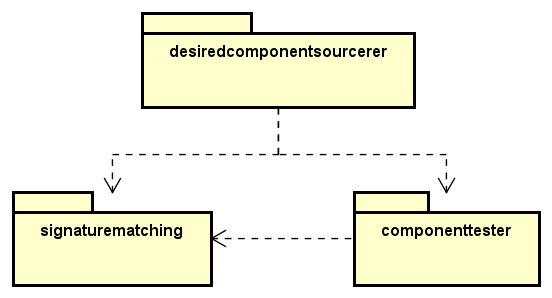
\includegraphics[scale=0.8]{cd_arch.png}
\caption{Architektur}
\label{cd_arch}
\end{figure}
\noindent
\\
Im weiteren Verlauf dieses Kapitels werden die \Gls{Modul}e einzeln beschrieben . Das Modul \emph{DesiredComponentSourcerer} ist dabei von den \Gls{Modul}en \emph{ComponentTester} und \emph{SignatureMatching} abhängig, während das Modul \emph{ComponentTester} lediglich vom Modul \emph{SignatureMatching} abhängig ist.
\\\\
Darüber hinaus, werden folgende externe Bibliotheken verwendet:
\begin{itemize}
%\item easymock 3.0 \cite{easymock}
\item cglib 3.3.0 \cite{cglib}
\item objenesis 3.1 \cite{objenesis}
\item junit 4.13.0 \cite{junit}
\end{itemize}
Auf die konkrete Verwendung der externen Bibliotheken wird in den detaillierteren Beschreibungen der einzelnen \Gls{Modul}e eingegangen.
\section{Modul: SignatureMatching}\label{impl_sigma}
\begin{figure}[h!]
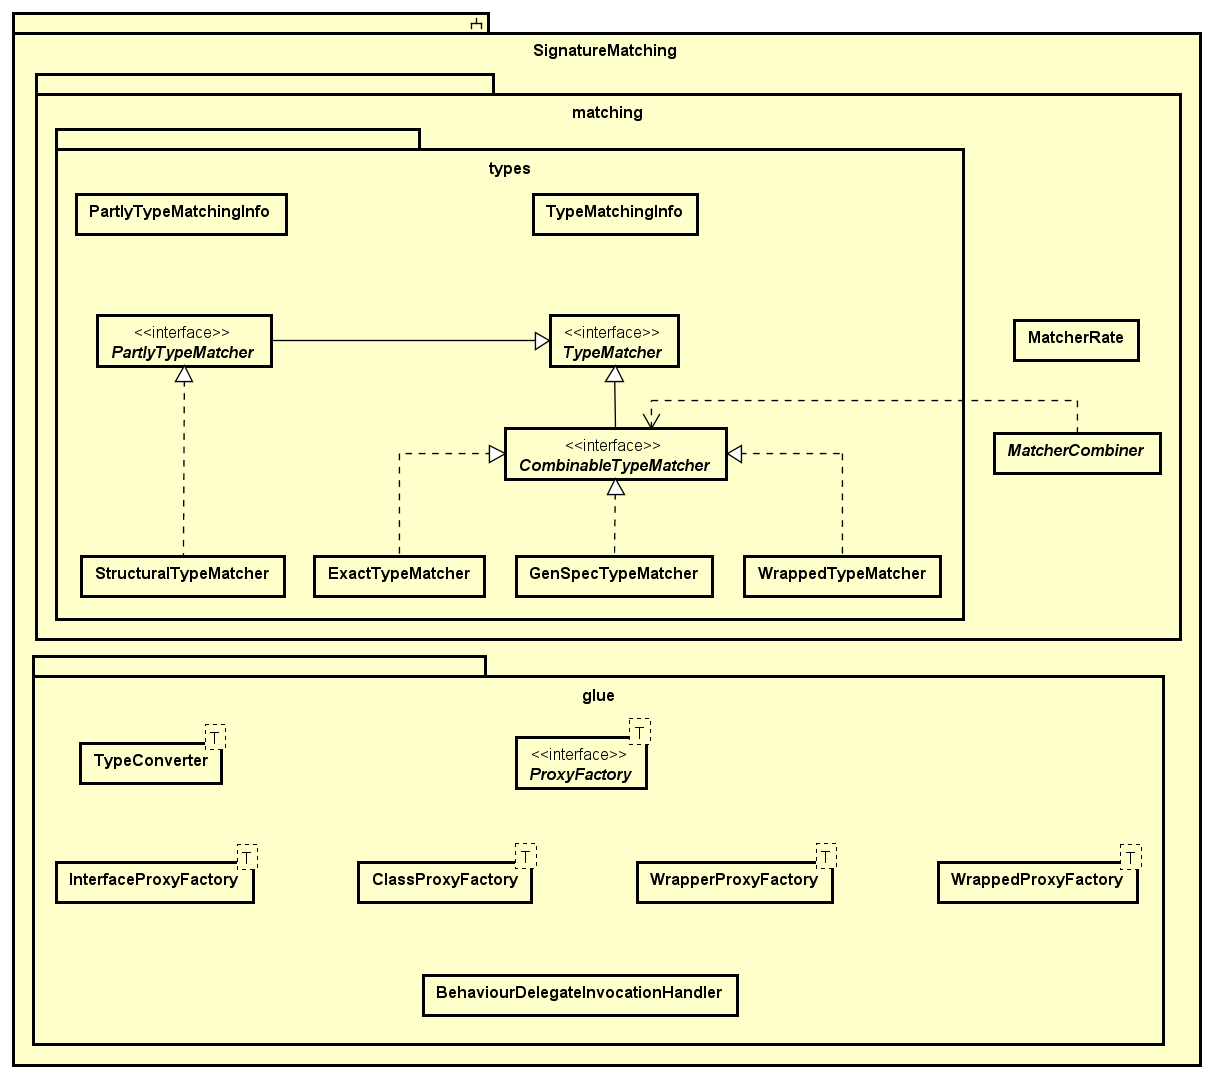
\includegraphics[scale=0.5]{cd_SigMa.png}
\caption{Modul: SignatureMatching}
\label{fig_cdSigMa}
\end{figure}
\noindent
In diesem \Gls{Modul} befinden sich zum einen die Implementierungen der Matcher, die in Abschnitt \ref{sec_matcher} formal beschrieben wurden und zum anderen die Implementierung der Generatoren für die \emph{Proxies}. In Abbildung \ref{fig_cdSigMa} sind die wichtigsten Klassen und \Gls{Interface}s dieses \Gls{Modul}s mit ihren Abhängigkeiten zueinander aufgeführt. Die Matcher befinden sich dabei im Package \emph{matching} und die Generatoren für die \emph{Proxies} in Form der Implementierungen des \Gls{Interface}s $\texttt{ProxyFactory}$ im Package \emph{glue}.
\\\\
Die in Abschnitt \ref{sec_matcher} beschriebenen Matcher und Generatoren wurden teilweise in einer Klasse zusammengefasst. Tabelle \ref{tab_matcher2impl} zeigt die Zuordnung von Matchern zu den jeweiligen Klassen, die die Implementierung dieser darstellen (Spalte: Matcher-Implementierung). Zudem sind in der Tabelle \ref{tab_matcher2impl} auch die Klassen ausgewiesen, die die Implementierung des Generators für den Proxy, der auf Basis des Matchers Anwendung findet, darstellen (Spalte: Generator-Implementierung).
\begin{table}[h!]
\centering
\begin{tabular}{|l|l|l|}
\hline
\hline
\textbf{Matcher} & \textbf{Matcher-Implementierung} & \textbf{Generator-Implementierung}\\
\hline
ExactTypeMatcher & $\texttt{ExactTypeMatcher}$ & $\texttt{ClassProxyFactory}$ \\
\hline
GenTypeMatcher & $\texttt{GenSpecTypeMatcher}$ & $\texttt{ClassProxyFactory}$\\
\hline
SpecTypeMatcher & $\texttt{GenSpecTypeMatcher}$ & $\texttt{ClassProxyFactory}$\\
\hline
ContentTypeMatcher & $\texttt{ContainerTypeMatcher}$ & $\texttt{ContentProxyFactory}$\\
\hline
ContainerTypeMatcher & $\texttt{ContainerTypeMatcher}$ & $\texttt{ContainerProxyFactory}$\\
\hline
StructuralTypeMatcher & $\texttt{StructuralTypeMatcher}$ & $\texttt{InterfaceProxyFactory}$\\
\hline
\hline
\end{tabular}
\caption{Zuordnung der Matcher zu den Matcher- und Generator-Implementierungen}
\end{table}\label{tab_matcher2impl}
\noindent
\\\\
Die Klasse $\texttt{StructuralTypeMatcher}$ nimmt bei den Matcher-Klassen eine Sonderstellung ein. Dies ist daran zu erkennen, dass dieser nicht das \Gls{Interface} $\texttt{TypeMatcher}$ implementiert. Das liegt daran, dass es sich bei diesem Matcher um den Einstiegspunkt der \emph{strukturellen Evaluation} handelt. Analog zum \emph{StructuralTypeMatcher} aus Abschnitt \ref{sec_matcher} wird in der Klasse $\texttt{StructuralTypeMatcher}$ auf die anderen Matcher bzw. Matcher-Klassen zugegriffen, was in Abbildung \ref{fig_cdSigMa} durch die Aggregation zwischen der Klasse $\texttt{StructuralTypeMatcher}$ und dem \Gls{Interface} $\texttt{TypeMatcher}$ angedeutet werden soll.
\\\\
Die übrigen Matcher-Klassen implementieren das \Gls{Interface} $\texttt{TypeMatcher}$ und können über die Methode $\texttt{combine}$ aus der Klasse $\texttt{MatcherCombinator}$ miteinander kombiniert werden\footnote{Ein Beispiel für die Kombination von Matchern ist im Anhang \ref{app_matchercombination} zu finden.}. 
\\\\
So kann eine Kombination mehrerer $\texttt{TypeMatcher}$, die wiederum von Typ $\texttt{TypeMatcher}$ ist, in der Klasse $\texttt{StructuralTypeMatcher}$ verwendet werden. Die konkrete $\texttt{TypeMatcher}$-Kombination, die im $\texttt{StructuralTypeMatcher}$ instanziiert wird, orientiert sich an den Ausführungen in Abschnitt \ref{sec_matcher} (siehe auch Anhang \ref{app_matchercombination}). Es ist aber zu erwähnen, dass die Verwendung weiterer Matcher, die in dieser Arbeit nicht definiert wurden, denkbar ist. Eine solche Erweiterung ließe sich leicht in dieses Modul über die Implementierung des \Gls{Interface}s $\texttt{TypeMatcher}$ und die Verwendung der Klasse $\texttt{MatcherCombiner}$ vornehmen.
\\\\
Alle Matcher-Implementierungen bieten die Möglichkeit, zu ermitteln, ob ein Matching zwischen zwei Typen besteht (siehe Klassendiagramme in Abbildungen \ref{fig_cdMatchingInfo} und \ref{fig_cdSingleMatchingInfo}). Dies erfolgt jeweils über die Methode $\texttt{matchesType}$. Über die Methode $\texttt{calculateMatchingInfos}$ werden die Informationen bzgl. der Methodendelegationen zwischen den beiden gematchten Typen ermittelt. Diese Informationen werden in einem Objekt der Klasse $\texttt{SingleMatchingInfo}$ bzw. $\texttt{MatchingInfo}$ zusammengetragen, welche in Abbildung \ref{fig_cdMatchingInfo} und \ref{fig_cdSingleMatchingInfo} detailliert dargestellt werden.
\begin{figure}[h!]
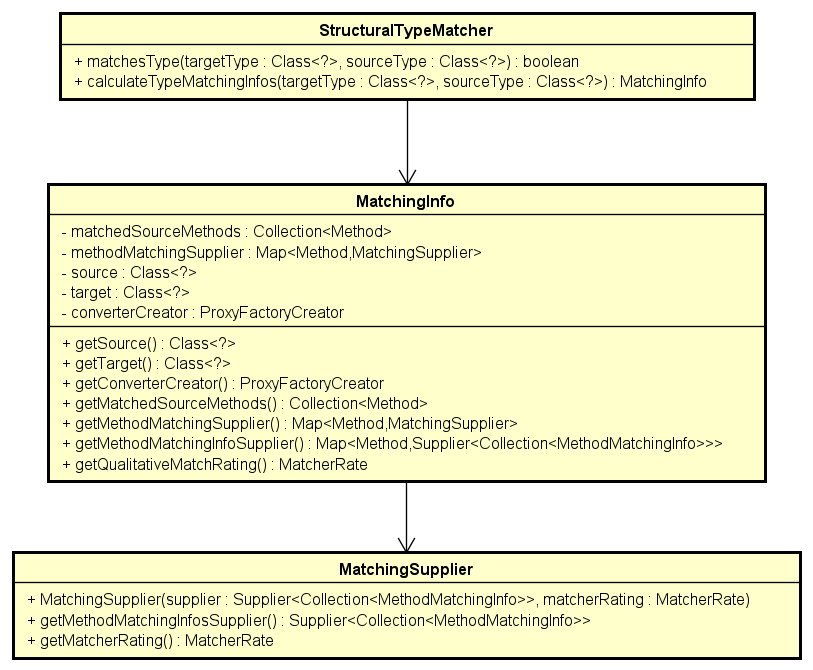
\includegraphics[scale=0.8]{cd_matchinginfo.png}
\caption{Klassendiagramm: $\texttt{StructuralTypeMatcher}$ und $\texttt{MatchingInfos}$}
\label{fig_cdMatchingInfo}
\end{figure}
\begin{figure}[h!]
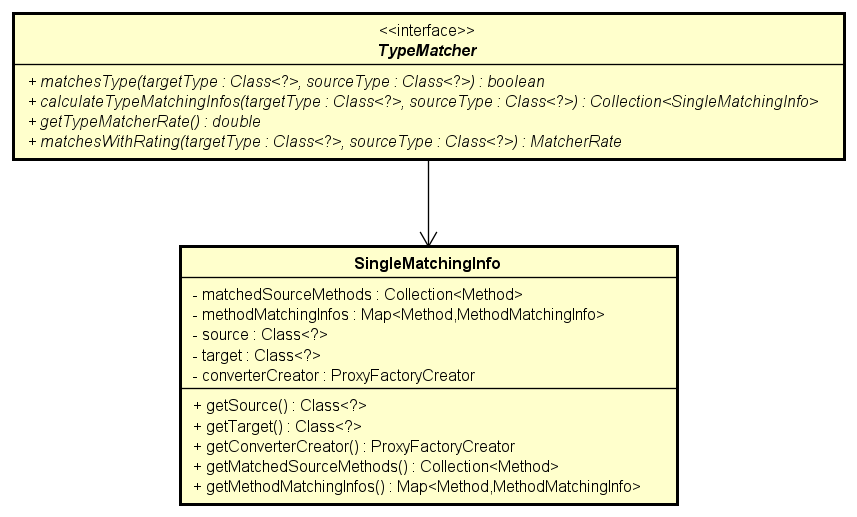
\includegraphics[scale=0.7]{cd_singlematchinginfo.png}
\caption{Klassendiagramm: $\texttt{TypeMatcher}$ und $\texttt{SingleMatchingInfo}$}
\label{fig_cdSingleMatchingInfo}
\end{figure}
\noindent
\\\\
Diese beiden Klassen unterscheiden sich lediglich bzgl. des Attributs in dem die Delegationsmethoden hinterlegt sind. Dabei handelt es sich auf Seiten der $\texttt{SingleMatchingInfo}$ um das Attribut $\texttt{methodMatchingInfos}$ und auf Seiten der $\texttt{MatchingInfo}$ um das Attribut $\texttt{methodMatchingSupplier}$. 
\\\\
Während ein Objekt der Klasse $\texttt{MatchingInfo}$ mehrere \emph{Delegationsmethoden} zu einer \emph{aufgerufenen Methoden} enthalten kann, darf ein Objekt der Klasse $\texttt{SingleMatchingInfo}$ lediglich eine \emph{Delegationsmethode} zu einer \emph{aufgerufenen Methode} enthalten (vgl. auch Abschnitt \ref{sec_matcher}). Zusätzlich zu erwähnen ist, dass die Informationen über die \emph{Delegationsmethoden} aus einer $\texttt{MatchingInfo}$ über einen $\texttt{MethodSupplier}$ überliefert werden.
\\\\
Eine Instanz der Klasse $\texttt{MethodSupplier}$ enthält zum einen ein $\texttt{MatcherRating}$ welches Informationen bzgl. des in Abschnitt \ref{sec_lmf} beschriebenen \emph{Matcherratings} beinhaltet. Zum anderen werden im Attribut $\texttt{methodMatchingInfo}$ in einem Objekt der Klasse $\texttt{MethodMatchingInfo}$ (siehe Abbildung \ref{cd_methodMatchingInfo}) die Informationen bzgl. der Delegation der \emph{aufgerufenen Methode} an die \emph{Delegationsmethode} hinterlegt. 
\\\\
Bezüglich der Klasse $\texttt{SingleMatchingInfo}$ ist noch das Attribut $\texttt{proxyFactoryCreator}$ zu beschreiben. Darin werden Informationen bzgl. der strukturellen Verbindung zwischen den gematchten Typen gehalten. 
\\\\
Für den \emph{ExactTypeMatcher}, den \emph{GenTypeMatcher} und den \emph{SpecTypeMatcher} wird dabei ein $\texttt{ProxyFactoryCreator}$ erzeugt, der in der Lage ist, eine $\texttt{ProxyFactory}$ für Typen zu erzeugen, die in einer nominalen Beziehung \footnote{Identität, Generalisierung, Spezialisierung} stehen. 
\\\\
Für den \emph{ContentTypeMatcher} und den \emph{ContainedTypeMatcher} hingegen, wird ein Objekt vom Typ $\texttt{ProxyFactoryCreator}$ erzeugt, der in der Lage ist, eine $\texttt{ProxyFactory}$ für Typen zu erzeugen, bei denen der eine Typ ein Attribut vom Typ des anderen enthält (vgl. mit Tabelle \ref{tab_matcher2impl}). Die erzeugten Objekte vom Typ $\texttt{ProxyFactory}$ werden bei der Generierung der \emph{Proxies} unter der Zuhilfenahme der Bibliotheken \emph{cglib} und \emph{objenesis} verwendet\footnote{Diese beiden Frameworks wurden verwendet, da die Erzeugung der \emph{Proxies} mit ihnen komfortabler ist, als mit den Mitteln die das JKD zur Verfügung stellt. Dies gilt insbesondere für die Erzeugung von \emph{Proxies} für Klassen, die mit dem Schlüsselwort $\texttt{final}$ versehen sind. (vgl. \cite{objenesis}, \cite{cglib})}.
\\\\
Der $\texttt{ProxyFactoryCreator}$ stellt damit eines der Bindeglieder zwischen der Package \emph{matching} und dem Package \emph{glue} innerhalb dieses \Gls{Modul}s her. Das zweite \Gls{artefakt}, welches als Bindeglied fungiert, ist die oben bereits erwähnte Klasse $\texttt{MethodMatchingInfo}$, deren Aufbau dem Klassendiagramm aus Abbildung \ref{cd_methodMatchingInfo} zu entnehmen ist.
\begin{figure}[h!]
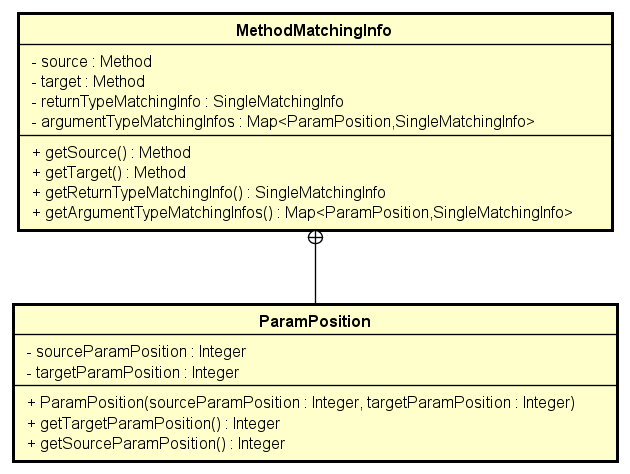
\includegraphics[scale=1.0]{cd_methodmatchinginfo.png}
\caption{Klassendiagramm: $\texttt{MethodMatchingInfo}$}
\label{cd_methodMatchingInfo}
\end{figure}
\noindent
\\\\
Ein Objekt der Klasse $\texttt{MethodMatchingInfo}$ enthält in den Attributen $\texttt{source}$ und $\texttt{target}$ je eine Methode. Dabei ist im Attribut $\texttt{source}$ die \emph{aufgerufene Methode} der \emph{Methoden-Delegation} und im Attribut $\texttt{target}$ die \emph{Delegationsmethode} hinterlegt. Darüber hinaus wird im Attribut $\texttt{returnTypeMatchingInfo}$ ein Objekt der Klasse $\texttt{SingleMatchingInfo}$ gehalten, welches alle notwendigen Informationen für das Erzeugen eines \emph{Proxies} des Rückgabetyps der \emph{aufgerufenen Methode} aus dem Rückgabetyp der \emph{Delegationsmethode} enthält.
\\\\
Analog dazu wird im Attribut $\texttt{argumentTypeMatchingInfos}$ eine Map, bestehend aus weiteren Objekten der Klasse $\texttt{SingleMatchingInfo}$ und jeweils einem Objekt der Klasse $\texttt{ParamPosition}$, gehalten. Diese Map enthält alle notwendigen Information für das Erzeugen eines \emph{Proxies} für die Parametertypen der \emph{Delegationsmethoden} aus den Parametertypen der \emph{aufgerufenen Methode}, sowie der Anpassung der Übergabeposition bei der Delegation der \emph{aufgerufenen Methode} (siehe auch Abschnitt \ref{sec:proxygram}).
\\\\
Um die \emph{Methoden-Delegationen} zu koordinieren, wird bei der Erzeugung des \emph{Proxies} in der jeweiligen $\texttt{ProxyFactory}$ für das \emph{Proxy}-Objekt ein $\texttt{InvocationHandler}$ instanziiert (vgl. \cite{invocationhandler}). Dieses \Gls{Interface} wird im \emph{glue}-Package durch die Klasse $\texttt{BehaviourDelegateInvocationHandler}$ implementiert, in der letztendlich die Koordination der \emph{Methoden-Delegationen} auf Basis der jeweiligen $\texttt{MethodMatchingInfo}$ spezifiziert ist.
\\\\
Um einen \emph{Proxy} basierend auf dem Matching zweier Typen zu erzeugen, steht die Klasse $\texttt{TypeConverter}$ zur Verfügung (siehe Abbildung \ref{cd_typeconverter}). Die Zugriffe innerhalb des Packages \emph{glue} als auch die Zugriffe von außerhalb verlangen jeweils ein Objekt der Klasse $\texttt{ConvertableBundle}$. Diese Klasse beschreibt eine Kombination mehrerer Objekte vom Typ $\texttt{ConvertableComponent}$, die als \emph{Target-Typen} des zu erzeugenden Proxy-Objektes fungieren sollen. Ein Objekt der Klasse $\texttt{ConvertableComponent}$ enthält eine Liste von Objekten vom Typ $\texttt{SingleMatchingInfo}$, die wie bereits erwähnt beschreiben, am welche Methode die Delegation erfolgen soll. Das Objekt im Attribut $\texttt{convertableObject}$ der $\texttt{ModuleMatchingInfo}$ beinhaltet das Objekt, auf dem die \emph{Delegationsmethode} aufgerufen werden soll.
\begin{figure}[h!]
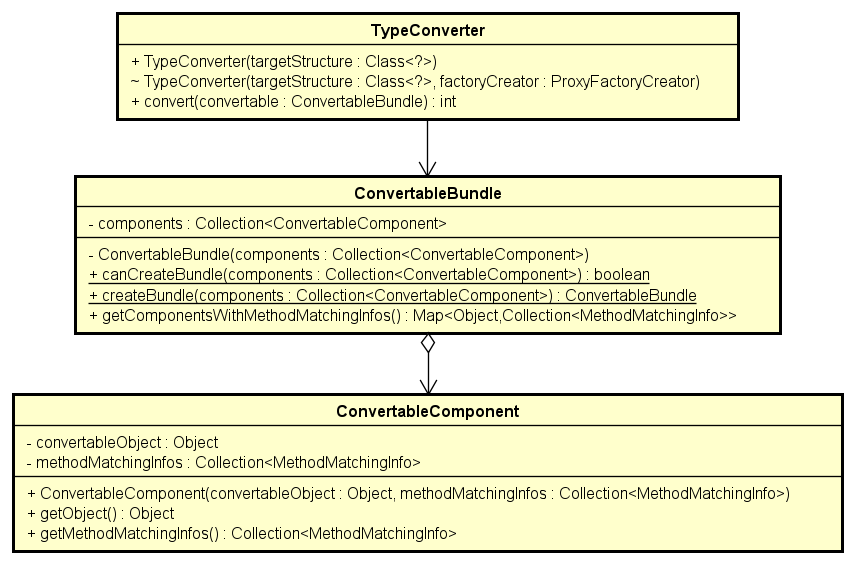
\includegraphics[scale=0.7]{cd_typeconverter.png}
\caption{Klassendiagramm: $\texttt{TypeConverter}$}
\label{cd_typeconverter}
\end{figure}

\section{Modul: ComponentTester}\label{sec_Impl_CT}
Dieses \Gls{Modul} ist für die Ausführung der vordefinierten Tests zuständig. Darüber hinaus bietet es die Möglichkeit, die vordefinierten Tests mit den \Gls{Interface}s, die den jeweiligen \emph{required Typ} darstellen, zu verbinden. Dabei sei davon auszugehen, dass ein \emph{required Typ} $R$ in Form eines \Gls{Interface}s existiert. Um die Tests für $R$ zu definieren, können eine oder mehrere Testklassen implementiert werden.
\\\\
Die Testklassen werden dabei in dem \Gls{Interface} $R$ über das Attribut $\texttt{testClasses}$ der Annotation $\texttt{RequiredTypeTestReference}$ angegeben (siehe Abbildung \ref{fig_cdCompTester} Package: \emph{API}). Ein Beispiel für die Deklaration eines solchen \Gls{Interface}s und den dazugehörigen Testklassen ist im Anhang \ref{app_interfacesAndTests} zu finden.
\\\\
Damit die Testmethoden in den Testklassen die in Abschnitt \ref{sec_testanforderungen} beschriebenen Eigenschaften aufweisen und durch das \emph{ComponentTester}-\Gls{Modul} ausfindig gemacht werden können, stehen mehrere \Gls{artefakt}e in dem \emph{API}- und dem \emph{SPI}-Package des \emph{ComponentTester}-\Gls{Modul}s bereit (siehe Abbildung \ref{fig_cdCompTester}).
\\\\
So muss jede Testklasse eine Methode bereitstellen, über die ein Objekt vom Typ $R$ in die Instanz der Testklasse injiziert werden kann.\footnote{auch genannt: Setter-Injection (vgl. \cite{setterinjection})} Diese Methode wird von dem \emph{ComponentTester}-\Gls{Modul} über die Annotation $\texttt{RequiredTypeInstanceSetter}$ gefunden. Von daher muss die Methode mit eben dieser Annotation markiert werden.
\begin{figure}[h!]
\centering
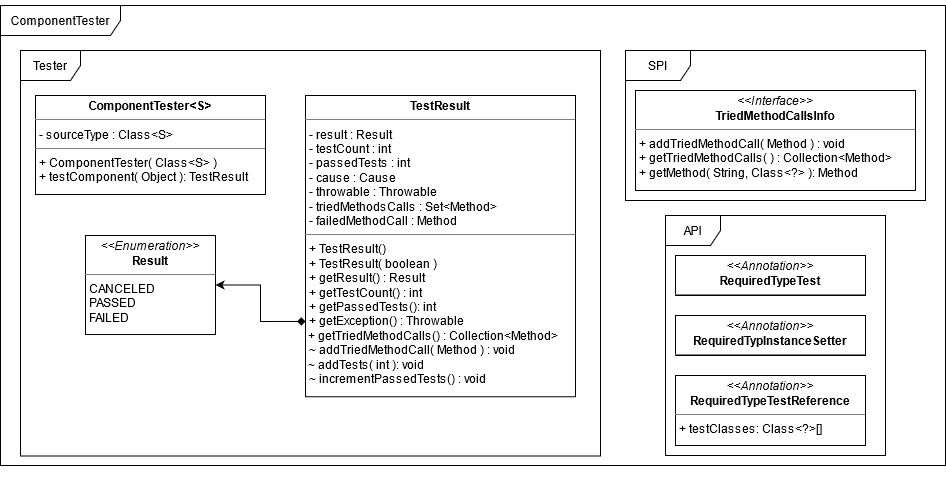
\includegraphics[scale=0.6]{pics/cd_ComponentTester.png}
\caption{Modul: ComponentTester}
\label{fig_cdCompTester}
\end{figure}
\noindent
Die Testmethoden müssen von der Sichtbarkeit her öffentlich ($\texttt{public}$) sein. Weiterhin dürfen die Testmethoden keine Parameter erwarten und müssen mit der Annotation $\texttt{RequiredTypeTest}$ markiert sein. Die Erwartungen innerhalb der Testmethoden müssen über die in JUnit 4 zur Verfügung stehenden Methoden aus der Klasse $\texttt{Assert}$ (siehe auch \cite{junit_api}) deklariert werden. Testdaten, die für alle Testmethoden innerhalb einer Testklasse zur Verfügung stehen sollen, können über Methoden bereitgestellt werden, die mit den durch die JUnit 4 Bibliothek bereitgestellten Annotationen $\texttt{Before}$ und $\texttt{After}$ (vgl. \cite{junit_api}) markiert wurden.
\\\\
Um die Reihenfolge der versuchten Aufrufe der Methoden, die von $R$ angeboten werden, zu verwalten\footnote{Das ist für die Heuristik \emph{BL\_NMC} notwendig. (vgl. auch Abschnitt \ref{sec_bl_nmc})}, muss die Testklasse das \Gls{Interface} $\texttt{TriedMethodCallsInfo}$ implementieren (siehe Abbildung \ref{fig_cdCompTester} Package: \emph{spi}). Dadurch wird die Implementierung der Methoden $\texttt{addTriedMethodCall}$ und $\texttt{getTriedMethodCalls}$ erzwungen. Die Methode $\texttt{getMethod}$ kann mit der Defaultimplementierung übernommen werden, sofern die in $R$ deklarierten Methoden über den Namen identifiziert werden können.
\\\\
Die Implementierung der Methoden $\texttt{addTriedMethodCall}$ und $\texttt{getTriedMethodCalls}$ hat so zu erfolgen, dass bei einem Aufruf der Methode $\texttt{addTriedMethodCall}$ der übergebene Parameter an eine Liste angefügt wird. Der Aufruf der Methode $\texttt{getTriedMethodCalls}$ liefert eben diese Liste als Rückgabewert. Weiterhin ist sicherzustellen, dass vor dem Aufruf einer Methode $m$ aus $R$ die Methode $\texttt{addTriedMethodCall}$ mit $m$ als Parameter aufgerufen wird. Im Anhang \ref{app_interfacesAndTests} sind mehrere Beispiele für die korrekte Implementierung von Testklassen zu finden (siehe Listings \ref{lst_testklassen_tei1} - \ref{lst_testklassen_tei7}).
\\\\
Die Durchführung der Tests, die für $R$ definiert wurde, wird über eine Instanz der Klasse $\texttt{ComponentTester}$ gestartet (siehe Abbildung \ref{fig_cdCompTester} Package: \emph{Tester}). In Abhängigkeit der in $R$ deklarierten Testklassen werden alle darin befindlichen Testmethoden mit einem \emph{Proxy} für $R$ durchgeführt, bis einer dieser Testfälle fehlschlägt. Der Aufrufer der Testdurchführung erhält dabei ein Objekt der Klasse $\texttt{TestResult}$ zurück (siehe Abbildung \ref{fig_cdCompTester}). In diesem Objekt sind die für die Auswertung des Testergebnisses relevanten Informationen vorhanden, auf die die Heuristiken \emph{PTTF} (siehe Abschnitt \ref{sec_pttf}) und \emph{BL\_NMC} (siehe Abschnitt \ref{sec_bl_nmc}) angewiesen sind.
\section{Modul: DesiredComponentSourcerer}\label{sec_impl_descos}
In diesem Modul ist die Implementierung der Exploration zu finden. Zum Starten der Exploration für ein \emph{required Typ} $R$ in Form eines \Gls{Interface}s muss zuerst eine Instanz der Klasse $\texttt{DesiredComponentFinder}$ erzeugt werden (genannt: \emph{Finder}). Dies erfolgt über einen Konstruktor, der ein Objekt der Klasse $\texttt{DesiredComponentFinderConfig}$ (genannt: \emph{Konfig}) erwartet (siehe Abbildung \ref{cd_descos}). 
\begin{figure}[h!]
\centering
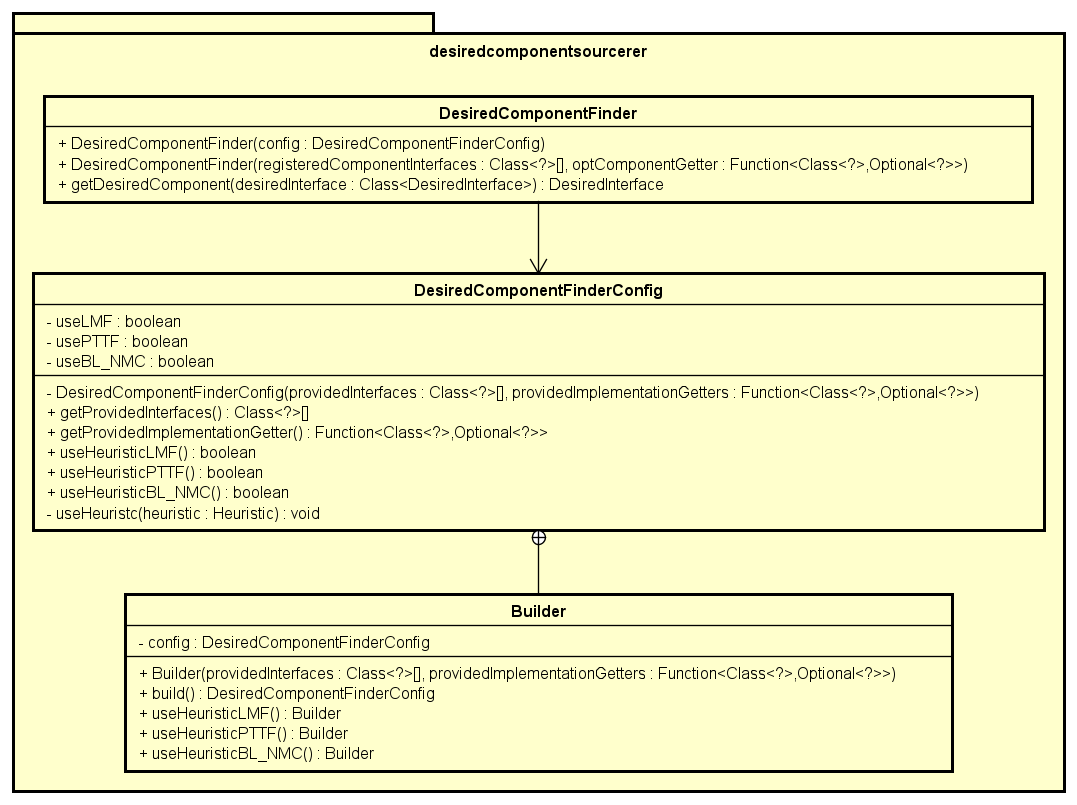
\includegraphics[scale=0.5]{cd_descos.png}
\caption{Modul: DesiredComponentSourcerer}
\label{cd_descos}
\end{figure}
\noindent
\\\\
Die Erzeugung einer solchen \emph{Konfig} erfolgt über einen Builder (Builder-Pattern). Dabei müssen zum Einen alle \emph{provided Typen} in Form einer Liste von \Gls{Interface}s angegeben werden. Zum Anderen wird eine Funktion ($\texttt{java.util.Function}$) gefordert, über die die Implementierungen der im Parameter übergebenen \Gls{Interface}s ermittelt werden können.
\\\\
Zum Zweck der gezielten Evaluation der Heuristiken in Kapitel \ref{chap_evaluation} kann über die \emph{Konfig} gesteuert werden, welche der in Abschnitt \ref{sec_heuristics} beschriebenen Heuristiken bei der Exploration verwendet werden sollen. Dies erfolgt über die in Abbildung \ref{cd_descos} ersichtlichen Methoden mit den Präfix $\texttt{useHeuristic*}$.
\\\\
Nach der Erzeugung des \emph{Finders} kann die Exploration über die Methode $\texttt{getDesiredComponent}$ mit der Übergabe des \emph{desired Interface} $R$ als Parameter gestartet werden. Im Anschluss wird die syntaktische Evaluation für alle \emph{provided Interfaces} durchgeführt. Hierzu wird ein Objekt vom $\texttt{StructuralTypeMatcher}$ aus dem \emph{SignatureMatching}-Modul verwendet\footnote{Dieses Objekt wird beim Instanziieren des \emph{Finders} erzeugt (siehe auch Anhang \ref{app_matchercombination}: Listing \ref{lst_matchermanager}).} und versucht die \emph{provided Typen} mit dem \emph{required Typ} zu matchen.
\\\\
Auf formaler Ebene gleicht dieser Schritt der Ausführung der Funktion $\mathit{cover(R,L)}$, wobei die in $L$ befindlichen \emph{provided Typen} auf die Typen, die dem \emph{Finder} bei der Instanziierung übergebenen wurden, beschränkt sind.
\\\\
Nach der strukturellen Evaluation, wird gemäß Abschnitt \ref{sec_semEval} die semantische Evaluation durchgeführt. Dabei werden zuerst die Proxies aus den Kombinationen der gematchten \emph{provided Typen}\footnote{Diese Kombinationen sind auf formaler Ebene Äquivalent zu den Elementen der Mengen aus $\mathit{cover(R,L)}$.} erzeugt, welche im Anschluss hinsichtlich der vordefinierten Tests zum \emph{required Typ} evaluiert werden. Dabei werden die Heuristiken, die in der \emph{Konfig} hinterlegt wurden, angewendet. Sofern bei der Exploration ein Proxy erfolgreich evaluiert wurde, wird dieser als Ergebnis des Aufrufs der Methode $\texttt{getDesiredComponent}$ zurückgegeben. 

\chapter{Untersuchungsergebnisse}\label{chap_evaluation}
In dem System, welches für die Evaluation der \Gls{Heuristik}en verwendet wird, sind insgesamt 891 \emph{provided Typen} (\emph{EJBs}) und 7 \emph{required Typen} enthalten. In \tabref{eIShort} sind die Namen der \emph{required Typen} zusammen mit jeweils einem Kürzel und den Namen der strukturell und semantisch matchenden Kombinationen von \emph{provided Typen} aufgeführt, die während des \emph{Explorationsprozesses} ermittelt werden sollen. Die Kürzel dienen im weiteren Verlauf der Identifizierung der \emph{required Typen}.
\begin{table}[h!]
\centering
\small
\begin{tabular}{|p{6cm}|p{1.5cm}|p{6.5cm}|}
\hline
\hline
\centering\textbf{required Typ} & \textbf{Kürzel} & \textbf{Kombination von provided Typen}\\
\hline
\hline
ElerFTFoerderprogrammeProvider & TEI1 & ElerFTStammdatenAuskunftService\\
\hline
FoerderprogrammeProvider & TEI2 & StammdatenAuskunftService\\
\hline
MinimalFoerderprogrammeProvider & TEI3 & StammdatenAuskunftService\\
\hline
IntubatingFireFighter & TEI4 & Doctor, FireFigher\\
\hline
IntubatingFreeing & TEI5 & Doctor, FireFigher\\
\hline
IntubatingPatientFireFighter & TEI6 & Doctor, FireFigher\\
\hline
KOFGPCProvider & TEI7 & ElerFTStammdatenAuskunftService, StammdatenAuskunftService\\
\hline
\hline
\end{tabular}
\caption{Required Typen mit Kürzeln und matchenden Kombinationen von provided Typen}
 \label{tab:eIShort}
\end{table}
\noindent
\\
Die Deklarationen der \emph{required Typen} und der \emph{provided Typen} aus \tabref{eIShort} sind im Anhang \ref{app_evalTypes} zu finden. Aufgrund der Geheimhaltungspflicht bzgl. der Implementierungsdetails kann auf die Deklaration der Java-Interfaces, die sich aus dieser Deklaration der \emph{required} und \emph{provided Typen} ableiten lassen, und deren Implementierungen in dieser Arbeit nicht genauer eingegangen werden.
\\\\
Um die Ergebnisse nachstellen zu können, kann die Implementierung, welche im Abschnitt \ref{sec_impl_descos} beschrieben wurde, mit einer beliebigen Bibliothek, welche sich ebenfalls durch die in Abschnitt \ref{sec:strukturTypen} beschriebene Struktur von Typen abbilden lässt, verwendet werden.

\section{Darstellung der Untersuchungsergebnisse}
Die Untersuchungsergebnisse werden in der Form von Vier-Felder-Tafeln dargestellt (Beispiel siehe \tabref{vft:beispiel}). Für jeden \emph{required Typ} wird eine Vier-Felder-Tafel für jeden Durchlauf der Schleife innerhalb der Methode $\texttt{semanticEval}$ der \emph{semantischen Evaluation} (siehe Abschnitt \ref{sec_semEval}) aufgezeigt. Aus der jeweiligen Tafel geht hervor, wie viele \emph{Proxies} über die Funktion $\mathit{targetSets}$ (vgl. Abschnitt \ref{sec_semEval}) in dem aktuellen Iterationsschritt erzeugt werden können. Der Wert, den die Iterationsvariable $\texttt{i}$ im betrachteten Durchlauf enthält, wird in der oberen rechten Ecke der Tafel abgebildet.
\\\\
In der Spalte ``positiv'' ist die Anzahl der \emph{Proxies} verzeichnet, die innerhalb des Durchlaufs erzeugt und geprüft wurden. Die Zahl in der Spalte ``negativ'' drückt hingegen aus, wie viele der möglichen \emph{Proxies} aufgrund bestimmter Kriterien (bzw. \Gls{Heuristik}en) nicht erzeugt wurden. 
\\\\
Die Zeile ``falsch'' beschreibt die Anzahl der möglichen \emph{Proxies}, welche die \emph{semantische Evaluation} nicht bestehen. Dementsprechend stellt die Zeile ``richtig'' die Anzahl der \emph{Proxies} dar, welche die \emph{semantischen Evaluation} bestehen.
\\\\
Da der \emph{Explorationsprozess} abgebrochen wird, sofern ein \emph{Proxy} die \emph{semantische Evaluation} besteht, ist in der Zelle ``positiv'' - ``richtig'' ein Wert von 0 oder 1 zu erwarten. Dementsprechend ist in der Zelle ``negativ'' - ``richtig'' immer der Wert 0 enthalten, denn ein \emph{Proxy}, der nicht erzeugt wurde, kann auch nicht positiv getestet werden.
\\\\
Aus Abschnitt \ref{sec_anzahlProxies} geht hervor, dass die Anzahl der \emph{Proxies}, die für einen \emph{required Typ} $R$ mit einer Menge von \emph{provided Typen} $T$ über die Funktion $\mathit{proxyCount(R,T)}$ näherungsweise bestimmt werden kann. Für eine vereinfachte Darstellung der Untersuchungsergebnisse bzgl. eines \emph{required Typs} $R$ aus einer Bibliothek $L$ mit $C = \mathit{cover(R,L)}$ und einem Iterationsschritt $i$ wird die Anzahl der \emph{Proxies} für die Anzahl $a$ von Mengen von \emph{provided Typen}, auf deren Basis die \emph{Proxies} erzeugt werden können, näherungsweise auch wie folgt beschrieben:
\begin{gather*}
p_i(a) := \begin{array}{l|l}
\sum_{k=1}^{a}\mathit{proxyCount(R,TM)} & \{\mathit{TM_1},...,\mathit{TM_a}\} = \mathit{targetSets(C,i)}  
\end{array}
\end{gather*}
\noindent
Diese Notation kommt jedoch nur bei der Darstellung der Untersuchungsergebnisse eines Iterationsschrittes zum Einsatz, in dem ein valider \emph{Proxy} gefunden wird. Für alle anderen Durchläufe ist die Anzahl der möglichen \emph{Proxies} bekannt und wird somit auch explizit dargestellt. 
\\\\
\tabref{vft:beispiel} zeigt ein Beispiel für eine solche Vier-Felder-Tafel, in der die Ergebnisse des 1. Iterationsschrittes dargestellt sind. Dabei wurden 11 \emph{Proxies} generiert und getestet. 10 dieser \emph{Proxies} bestanden die \emph{semantische Evaluation} nicht. Da in diesem Beispiel ein \emph{Proxy} die \emph{semantische Evaluation} bestand, und der \emph{Explorationsprozess} anschließend beendet wurde, mussten die übrigen \emph{Proxies}, die auf Basis der insgesamt 20 Kombinationen von \emph{provided Typen} hätten erzeugt werden können, nicht generiert und damit auch nicht getestet werden.
\vft{1}{10}{$p_1(20)-11$}{1}{0}{Beispiel: Vier-Felder-Tafel}{vft:beispiel}


\section{Ausgangspunkt}\label{sec_ausgangspunkt}
Für einen \emph{reqiured Typ} können mehrere \emph{provided Typen} gefunden werden, auf deren Basis ein \emph{Proxy} erzeugt werden kann. \tabref{amountMatchedInterfaces} zeigt die Anzahl der \emph{provided Typen}, zu denen der jeweilige \emph{required Typ} über den \emph{StructuralTypeMatcher} gematcht werden kann\footnote{Strukturelle Übereinstimmung}. Diese kommen einzeln oder in Kombination für die \emph{semantische Evaluation} in Frage.
\begin{table}[H]
\centering
\small
\singlespacing
			\begin{tabular}[c]{|>{\centering\arraybackslash}p{2cm}|>{\centering\arraybackslash}p{5cm}|}
			\hline
			\hline
				 \textbf{Required Typ} & \textbf{Anzahl strukturell übereinstimmender provided Typ} \\
				\hline\hline
				TEI1 & 221 \\
				\hline
				TEI2 & 272\\
				\hline
				TEI3 & 268\\
				\hline
				TEI4 & 75\\
				\hline
				TEI5 & 75\\
				\hline
				TEI6 & 53\\
				\hline
				TEI7 & 346\\				
				\hline
				\hline
			\end{tabular} 
 \caption{Anzahl strukturell gematchten provided Typen für die Evaluation}
 \label{tab:amountMatchedInterfaces}
\onehalfspacing
\end{table}
\noindent
Die \tabsrefs{tmr_start_tei1}{tmr_start_tei7_2} zeigen die Vier-Felder-Tafeln, in denen die Ergebnisse der benötigten Iterationen innerhalb der \emph{semantischen Evaluation} für jeden der \emph{required Typen} aus \tabref{amountMatchedInterfaces}. Dabei wurden keine \Gls{Heuristik}en verwendet. Somit stellt dies den Ausgangspunkt für die weitere Evaluation der \Gls{Heuristik}en dar.
\begin{multicols}{3}
\vft{1}{233}{$p_1(44)-234$}{1}{0}{Ausgangspunkt für TEI1}{tmr_start_tei1}\columnbreak
\vft{1}{9389}{$p_1(55)-9399$}{1}{0}{Ausgangspunkt für TEI2}{tmr_start_tei2}\columnbreak
\vft{1}{8364}{$p_1(50)-8365$}{1}{0}{Ausgangspunkt für TEI3}{tmr_start_tei3}
\end{multicols}
\begin{multicols}{2}
\vft{1}{$1174$}{0}{0}{0}{Ausgangspunkt für TEI4 1.~\mbox{Durchlauf}}{tmr_start_tei4_1}\columnbreak
\vft{2}{56766}{$p_2(2247)-56767$}{1}{0}{Ausgangspunkt für TEI4 2.~\mbox{Durchlauf}}{tmr_start_tei4_2}
\end{multicols}
\begin{multicols}{2}
\vft{1}{$4984$}{0}{0}{0}{Ausgangspunkt für TEI5 1.~Durchlauf}{tmr_start_tei5_1}\columnbreak
\vft{2}{244479}{$p_2(2775)-244480$}{1}{0}{Ausgangspunkt für TEI5 2.~\mbox{Durchlauf}}{tmr_start_tei5_2}
\end{multicols}
\begin{multicols}{2}
\vft{1}{$1051$}{0}{0}{0}{Ausgangspunkt für TEI6 1.~\mbox{Durchlauf}}{tmr_start_tei6_1}
\columnbreak
\vft{2}{43360}{$p_2(1323)-43361$}{1}{0}{Ausgangspunkt für TEI6 2.~\mbox{Durchlauf}}{tmr_start_tei6_2}
\end{multicols}
\begin{multicols}{2}
\vft{1}{$161294$}{0}{0}{0}{Ausgangspunkt für TEI7 1.~\mbox{Durchlauf}}{tmr_start_tei7_1}
\columnbreak
\vft{2}{7764501}{$p_2(52150)-7764502$}{1}{0}{Ausgangspunkt für TEI7 2.~\mbox{Durchlauf}}{tmr_start_tei7_2}
\end{multicols}
\noindent
Für die \emph{required Typen} \emph{TEI4}-\emph{TEI7} werden zwei Durchläufe benötigt, da die Tests nur von einem \emph{Proxy} bestanden werden, der aus einer Kombination zweier \emph{provided Typen} erzeugt wurde (siehe auch \tabref{eIShort}).

\section{Ergebnisse für die Heuristik LMF}\label{sec_evalLMF}
In Bezug auf die Heuristik \emph{LMF} gilt es nicht nur zu evaluieren, ob die Suche nach einem Proxy, der die vordefinierten Tests besteht, beschleunigt werden kann, sondern auch, mit welcher Variante zur Bestimmung des Matcherratings (vgl. Abschnitt \ref{sec_lmf}) die besten Ergebnisse erzielt werden können. 
\\\\
Hierzu wird die Exploration für alle der oben genannten \emph{required Typen} für jede Variante zur Bestimmung der Matcherratings durchgeführt (siehe Abschnitt \ref{sec_lmf} Tabelle \ref{tab_matcherratingvarianten}). Im folgenden Verlauf wird lediglich auf die Variante eingegangen, die die besten Ergebnisse hervorgebracht hat. Die Ergebnisse unter Verwendung der übrigen Varianten sind im Anhang \ref{app_matcherratingEval} zu finden.
\\\\
Die Variante \emph{1.1} (vgl. Tabelle \ref{tab_matcherratingvarianten}) erbrachte die besten Ergebnisse. Die folgenden Vier-Felder-Tafeln zeigen die Ergebnisse mit dieser Variante zur Bestimmung der Matcherratings für die \emph{required Typen} \emph{TEI1}-\emph{TEI3} auf.
\begin{multicols}{3}
\vft{1}{5}{$p(44)-6$}{1}{0}{Ergebnisse \emph{LMF} mit Variante 1.1 für TEI1 \\1. Durchlauf}{lmf11_TEI1_1}
\vft{1}{1889}{$p(55)-1890$}{1}{0}{Ergebnisse \emph{LMF} mit Variante 1.1 für TEI2 1.~\mbox{Durchlauf}}{lmf11_TEI2_1}
\vft{1}{1463}{$p(50)-1464$}{1}{0}{Ergebnisse \emph{LMF} mit Variante 1.1 für TEI3 1.~\mbox{Durchlauf}}{lmf11_TEI3_1}
\end{multicols}
\noindent
Die Ergebnisse für die \emph{required Typen} \emph{TEI4}-\emph{TEI7} zeigen die folgenden Vier-Felder-Tafeln. 
\begin{multicols}{2}
\vft{1}{$1174$}{0}{0}{0}{Ergebnisse \emph{LMF} mit Variante 1.1 für TEI4 1.~\mbox{Durchlauf}}{lmf11_TEI4_1}
\vft{2}{2}{$p(2247)-3$}{1}{0}{Ergebnisse \emph{LMF} mit Variante 1.1 für TEI4 2.~\mbox{Durchlauf}}{lmf11_TEI4_2}
\end{multicols}

\begin{multicols}{2}
\vft{1}{$4984$}{0}{0}{0}{Ergebnisse \emph{LMF} mit Variante 1.1 für TEI5 1.~\mbox{Durchlauf}}{lmf11_TEI5_1}
\vft{2}{32}{$p(2775)-33$}{1}{0}{Ergebnisse \emph{LMF} mit Variante 1.1 für TEI5 2.~\mbox{Durchlauf}}{lmf11_TEI5_2}
\end{multicols}

\begin{multicols}{2}
\vft{1}{$1051$}{0}{0}{0}{Ergebnisse \emph{LMF} mit Variante 1.1 für TEI6 1.~\mbox{Durchlauf}}{lmf11_TEI6_1}
\vft{2}{0}{$p(1323)-1$}{1}{0}{Ergebnisse \emph{LMF} mit Variante 1.1 für TEI6 2.~\mbox{Durchlauf}}{lmf11_TEI6_2}
\end{multicols}

\begin{multicols}{2}
\vft{1}{$161294$}{0}{0}{0}{Ergebnisse \emph{LMF} mit Variante 1.1 für TEI7 1.~\mbox{Durchlauf}}{lmf11_TEI7_1}
\vft{2}{7641}{$p(52150)-7642$}{1}{0}{Ergebnisse \emph{LMF} mit Variante 1.1 für TEI7 2.~\mbox{Durchlauf}}{lmf11_TEI7_2}
\end{multicols}
\noindent
Folgendes kann aus diesen Ergebnissen abgeleitet werden:
\begin{enumerate}
\item Die Heuristik \emph{LMF} erzielt eine Reduktion der zu erzeugenden Proxies. Dies wird durch einen Vergleich der Spalte ``positiv'' innerhalb der Vier-Felder-Tafeln zum jeweiligen \emph{required Typ} belegt.

\item Die Heuristik \emph{LMF} hat keine Auswirkung auf einen Durchlauf, in dem kein Proxy erzeugt wird, mit dem die semantischen Tests erfolgreich durchgeführt werden können. Dies kann durch einen Vergleich des ersten Durchlaufs für die \emph{required Typen} \emph{TEI4}-\emph{TEI7} im Ausgangspunkt (Tabellen \ref{tab:tmr_start_tei4_1}, \ref{tab:tmr_start_tei5_1}, \ref{tab:tmr_start_tei6_1} und \ref{tab:tmr_start_tei6_1}) mit dem ersten Durchlauf unter Anwendung der Heuristik (Tabellen \ref{tab:lmf11_TEI4_1}, \ref{tab:lmf11_TEI5_1}, \ref{tab:lmf11_TEI6_1} und \ref{tab:lmf11_TEI7_1}) festgestellt werden.
\end{enumerate}



%Aus diesen Ergebnissen lässt sich folgendes ableiten:
%\begin{enumerate}
%\item Das Akkumulationsverfahren Nummer 3. (Minimum) führt sowohl für die Typ- und Methoden-Konvertierungsvarianten zu schlechteren Ergebnissen als die anderen drei Akkumulationsverfahren. Es sollte daher für die Heuristik TMR\_Quant nicht verwendet werden.
%\item Die Ergebnisse von 1-2 und 3-2 unterscheiden sich nur geringfügig, obwohl bei 3-2 das Akkumulationsverfahren Nummer 3. zum Einsatz kam. Dies konnte auch bei anderen Kombinationen festgestellt werden, bei denen das 3. Akkumulationsverfahren für die Akkumulation des Type-Matcher Ratings der Typ-Konvertierungsvariante verwendet wurde. Das lässt vermuten, dass die Beachtung des Type-Matcher Ratings einer ganzen Typ-Konvertierungsvariante weitgehend unerheblich für die Heuristik TMR\_Quant ist.
%, wenn das Type-Matcher Rating je Methoden-Konvertierungsvarianten über ein entsprechend gutes Akkumulationsverfahren ermittelt wurde. 
%Dies ist jedoch darauf zurückzuführen, dass das Type-Matcher Rating je Methoden-Konvertierungsvariante die Parameter für die Ermittlung des Type-Matcher Ratings einer Typ-Konvertierungsvariante darstellen.
%\item An den Ergebnissen zu den erwarteten Interfaces TEI4-TEI6 ist zu erkennen, dass die Heuristik TMR\_Quant keinen Einfluss auf den 1. Durchlauf hat. Daraus kann geschlussfolgert werden, dass die Heuristik nur in dem Durchlauf einen Gewinn bringt, in dem auch eine passende benötigte Komponente gefunden werden kann. 
%\end{enumerate}
%Aufgrund der Ergebnisse stehen für die weitere Verwendung der Heuristik TMR\_Qual mehrere Kombinationen von Akkumulationsverfahren zur Auswahl. Die Entscheidung fällt aufgrund der etwas geringeren Komplexität auf die Kombination 1-2. 

\section{Ergebnisse für die Heuristik PTTF}\label{sec_evalPTTF}
Für die \Gls{Heuristik} \emph{PTTF} gilt es zu evaluieren, ob die Suche nach einem \emph{Proxy}, der die vordefinierten Tests besteht, beschleunigt werden kann. Hierzu wird der \emph{Explorationsprozess} für alle in Tabelle \ref{tab:eIShort} genannten \emph{required Typen} unter der Verwendung der in Abschnitt \ref{sec_pttf} beschriebenen \Gls{Heuristik} durchgeführt.
\\\\
Die folgenden Vier-Felder-Tafeln zeigen die Ergebnisse für die \emph{required Typen} \emph{TEI1}-\emph{TEI7} auf.
\begin{multicols}{3}
\vft{1}{29}{$p_1(44)-30$}{1}{0}{Ergebnisse \emph{PTTF} für TEI1 1.~\mbox{Durchlauf}}{pttf_TEI1_1}
\vft{1}{5544}{$p_1(55)-5545$}{1}{0}{Ergebnisse \emph{PTTF} für TEI2 1.~\mbox{Durchlauf}}{pttf_TEI2_1}
\vft{1}{4761}{$p_1(50)-4762$}{1}{0}{Ergebnisse \emph{PTTF} für TEI3 1.~\mbox{Durchlauf}}{pttf_TEI3_1}
\end{multicols}

\begin{multicols}{2}
\vft{1}{$1174$}{0}{0}{0}{Ergebnisse \emph{PTTF} für TEI4 1.~\mbox{Durchlauf}}{pttf_TEI4_1}
\vft{2}{466}{$p_2(2247)-467$}{1}{0}{Ergebnisse \emph{PTTF} für TEI4 2.~\mbox{Durchlauf}}{pttf_TEI4_2}
\end{multicols}
\pagebreak
\begin{multicols}{2}
\vft{1}{$4984$}{0}{0}{0}{Ergebnisse \emph{PTTF} für TEI5 1.~\mbox{Durchlauf}}{pttf_TEI5_1}
\vft{2}{2172}{$p_2(2775)-2173$}{1}{0}{Ergebnisse \emph{PTTF} für TEI5 2.~\mbox{Durchlauf}}{pttf_TEI5_2}
\end{multicols}

\begin{multicols}{2}
\vft{1}{$1051$}{0}{0}{0}{Ergebnisse \emph{PTTF} für TEI6 1.~\mbox{Durchlauf}}{pttf_TEI6_1}
\vft{2}{13122}{$p_2(1323)-13123$}{1}{0}{Ergebnisse \emph{PTTF} für TEI6 2.~\mbox{Durchlauf}}{pttf_TEI6_2}
\end{multicols}

\begin{multicols}{2}
\vft{1}{$161294$}{0}{0}{0}{Ergebnisse \emph{PTTF} für TEI7 1.~\mbox{Durchlauf}}{pttf_TEI7_1}
\vft{2}{149961}{$p_2(52150)-149962$}{1}{0}{Ergebnisse \emph{PTTF} für TEI7 2.~\mbox{Durchlauf}}{pttf_TEI7_2}
\end{multicols}
\newpage
\noindent
Folgendes kann aus diesen Ergebnissen abgeleitet werden:
\begin{enumerate}
\item Die \Gls{Heuristik} \emph{PTTF} erzielt im Vergleich zum Ausgangspunkt (Abschnitt \ref{sec_ausgangspunkt}) für jeden \emph{required Typ} eine weitere Reduktion der zu prüfenden \emph{Proxies}.

\item Die Heuristik \emph{PTTF} hat keine Auswirkung auf einen Durchlauf, in dem kein \emph{Proxy} erzeugt wird, mit dem die vordefinierten Tests erfolgreich durchgeführt werden können. Dies kann durch einen Vergleich des ersten Durchlaufs für den \emph{required Typ} \emph{TEI4}-\emph{TEI7} im Ausgangspunkt (Tabelle \ref{tab:tmr_start_tei4_1}, \ref{tab:tmr_start_tei5_1}, \ref{tab:tmr_start_tei6_1} und \ref{tab:tmr_start_tei6_1}) mit dem ersten Durchlauf unter Anwendung der Heuristik (Tabellen \ref{tab:pttf_TEI4_1}, \ref{tab:pttf_TEI5_1}, \ref{tab:pttf_TEI6_1} und \ref{tab:pttf_TEI7_1}) festgestellt werden. Aus diesem Grund kommt die in Punkt 1 beschriebene Reduktion erst im jeweils letzten Durchlauf zum Tragen.
\end{enumerate}
\section{Ergebnisse für die Heuristik BL\_NMC}\label{sec_evalBLNMC}
Für die \Gls{Heuristik} \emph{BL\_NMC} gilt es zu evaluieren, ob die Suche nach einem \emph{Proxy}, der die vordefinierten Tests besteht, beschleunigt werden kann. Hierzu wird der \emph{Explorationsprozess} für alle in Tabelle \ref{tab:eIShort}genannten \emph{required Typen} unter der Verwendung der in Abschnitt \ref{sec_bl_nmc} beschriebenen \gls{Heuristik} durchgeführt.
\\\\
Die folgenden Vier-Felder-Tafeln zeigen die Ergebnisse für die \emph{required Typen} \emph{TEI1}-\emph{TEI7} auf.
\begin{multicols}{3}
\vft{1}{105}{$p_1(44)-106$}{1}{0}{Ergebnisse \emph{BL\_NMC} für TEI1 1.~\mbox{Durchlauf}}{blnmc_TEI1_1}
\vft{1}{342}{$p_1(55)-343$}{1}{0}{Ergebnisse \emph{BL\_NMC} für TEI2 1.~\mbox{Durchlauf}}{blnmc_TEI2_1}
\vft{1}{357}{$p_1(50)-358$}{1}{0}{Ergebnisse \emph{BL\_NMC} für TEI3 1.~\mbox{Durchlauf}}{blnmc_TEI3_1}
\end{multicols}

\begin{multicols}{2}
\vft{1}{120}{$1054$}{0}{0}{Ergebnisse \emph{BL\_NMC} für TEI4 1.~\mbox{Durchlauf}}{blnmc_TEI4_1}
\vft{2}{442}{$p_2(2247)-443$}{1}{0}{Ergebnisse \emph{BL\_NMC} für TEI4 2.~\mbox{Durchlauf}}{blnmc_TEI4_2}
\end{multicols}

\begin{multicols}{2}
\vft{1}{550}{$4434$}{0}{0}{Ergebnisse \emph{BL\_NMC} für TEI5 1.~\mbox{Durchlauf}}{blnmc_TEI5_1}
\vft{2}{1304}{$p_2(2775)-1305$}{1}{0}{Ergebnisse \emph{BL\_NMC} für TEI5 2.~\mbox{Durchlauf}}{blnmc_TEI5_2}
\end{multicols}
\pagebreak
\begin{multicols}{2}
\vft{1}{366}{$685$}{0}{0}{Ergebnisse \emph{BL\_NMC} für TEI6 1.~\mbox{Durchlauf}}{blnmc_TEI6_1}
\vft{2}{204}{$p_2(1323)-205$}{1}{0}{Ergebnisse \emph{BL\_NMC} für TEI6 2.~\mbox{Durchlauf}}{blnmc_TEI6_2}
\end{multicols}

\begin{multicols}{2}
\vft{1}{1051}{$160243$}{0}{0}{Ergebnisse \emph{BL\_NMC} für TEI7 1.~\mbox{Durchlauf}}{blnmc_TEI7_1}
\vft{2}{135089}{$p_2(52150)-135090$}{1}{0}{Ergebnisse \emph{BL\_NMC} für TEI7 2.~\mbox{Durchlauf}}{blnmc_TEI7_2}
\end{multicols}

Folgendes kann aus diesen Ergebnissen abgeleitet werden:
\begin{enumerate}
\item Die \Gls{Heuristik} \emph{BL\_NMC} erzielt im Vergleich zum Ausgangspunkt (Abschnitt \ref{sec_ausgangspunkt}) für jeden \emph{required Typ} eine weitere Reduktion der zu prüfenden \emph{Proxies}.

\item Die Heuristik \emph{BL\_NMC} hat das Potential jeden Durchlauf innerhalb der \emph{semantischen Evaluation} zu beschleunigen. Für den jeweils ersten Durchlauf kann dies durch einen Vergleich der Tabellen \ref{tab:tmr_start_tei1}, \ref{tab:tmr_start_tei2}, \ref{tab:tmr_start_tei3}, \ref{tab:tmr_start_tei4_1}, \ref{tab:tmr_start_tei5_1}, \ref{tab:tmr_start_tei6_1} und \ref{tab:tmr_start_tei7_1} zum Ausgangspunkt mit den Tabellen \ref{tab:blnmc_TEI1_1}, \ref{tab:blnmc_TEI2_1}, \ref{tab:blnmc_TEI3_1}, \ref{tab:blnmc_TEI4_1}, \ref{tab:blnmc_TEI5_1}, \ref{tab:blnmc_TEI6_1} und \ref{tab:blnmc_TEI7_1} festgestellt werden. Ein Vergleich der Tabelle \ref{tab:tmr_start_tei4_2}, \ref{tab:tmr_start_tei5_2}, \ref{tab:tmr_start_tei6_2} und \ref{tab:tmr_start_tei7_2} im Ausgangspunkt mit den Tabellen \ref{tab:blnmc_TEI4_2}, \ref{tab:blnmc_TEI5_2}, \ref{tab:blnmc_TEI6_2} und \ref{tab:blnmc_TEI7_2} belegt dies für den zweiten Durchlauf auf.
\end{enumerate}

\noindent
\\\\
Aus den Ergebnissen, die in den Abschnitten \ref{sec_evalLMF} - \ref{sec_evalBLNMC} beschrieben wurden, lässt sich je \emph{required Typ} eine Rangfolge der vorgestellten \Gls{Heuristik}en erstellen. Diese Rangfolge kann Tabelle \ref{tab_rankingSingle} entnommen werden. Dabei gilt, dass die \Gls{Heuristik}, mit der am wenigsten \emph{Proxies} generiert und geprüft werden mussten, den ersten Platz einnimmt. 
\begin{table}[!h]
\centering
\begin{tabular}{|l|c|c|c|c|c|c|c|}
\hline
\hline
\textbf{Heuristik/Required Typ} & \textbf{TEI1} & \textbf{TEI2}& \textbf{TEI3}& \textbf{TEI4}& \textbf{TEI5}& \textbf{TEI6}& \textbf{TEI7}\\
\hline
\hline
LMF  &1.&2.&2.&2.&2.&2.&2.\\
\hline
PTTF  &3. &3.&3.&3.&3.&3.&3. \\
\hline
BL\_NMC & 2. &1. &1. &1. &1.&1.&1.\\
\hline
\hline
\end{tabular}
\caption{Rangfolge der Heuristiken (Einzelbetrachtung)}
\label{tab_rankingSingle}
\end{table}


\section{Ergebnisse für die Kombination der Heuristiken}\label{sec_evalKombis}
Im vorherigen Abschnitt wurde gezeigt, dass der \emph{Explorationsprozess} durch jede der beschriebenen \Gls{Heuristik}en beschleunigt werden kann. Dabei wurde der \emph{Explorationsprozess} mit jeweils einer der \Gls{Heuristik}en durchgeführt. In den folgenden Abschnitten soll evaluiert werden, ob die Verwendung einer Kombination der einzelnen \Gls{Heuristik}en während des \emph{Explorationsprozesses} einen zusätzlichen Vorteil bringt.
\\\\
Hierzu werden die Ergebnisse aller Kombinationen der einzelnen \Gls{Heuristik}en aufgeführt und im Anschluss bewertet.
\subsection{Kombination: LMF + PTTF}\label{sec_evalLMFPTTF}
Die folgenden Vier-Felder Tafeln zeigen die Ergebnisse mit der Kombination der \Gls{Heuristik}en \emph{LMF} und \emph{PTTF}.
\begin{multicols}{3}
\vft{1}{5}{$p_1(44)-6$}{1}{0}{Ergebnisse \emph{LMF} + \emph{PTTF} für TEI1}{lmfpttf_TEI1_1}\columnbreak
\vft{1}{1877}{$p_1(55)-1878$}{1}{0}{Ergebnisse \emph{LMF} + \emph{PTTF} für TEI2 1. Durchlauf}{lmfpttf_TEI2_1}\columnbreak
\vft{1}{1473}{$p_1(50)-1474$}{1}{0}{Ergebnisse \emph{LMF} + \emph{PTTF} für TEI3 1. Durchlauf}{lmfpttf_TEI3_1}
\end{multicols}

\begin{multicols}{2}
\vft{1}{$1174$}{0}{0}{0}{Ergebnisse \emph{LMF} + \emph{PTTF} für TEI4 1. Durchlauf}{lmfpttf_TEI4_1}\columnbreak
\vft{2}{4}{$p_2(2247)-5$}{1}{0}{Ergebnisse \emph{LMF} + \emph{PTTF} für TEI4 2. Durchlauf}{lmfpttf_TEI4_2}
\end{multicols}

\begin{multicols}{2}
\vft{1}{$4984$}{0}{0}{0}{Ergebnisse \emph{LMF} + \emph{PTTF} für TEI5 1. Durchlauf}{lmfpttf_TEI5_1}\columnbreak
\vft{2}{34}{$p_2(2346)-35$}{1}{0}{Ergebnisse \emph{LMF} + \emph{PTTF} für TEI5 2. Durchlauf}{lmfpttf_TEI5_2}
\end{multicols}

\begin{multicols}{2}
\vft{1}{$1051$}{0}{0}{0}{Ergebnisse \emph{LMF} + \emph{PTTF} für TEI6 1. Durchlauf}{lmfpttf_TEI6_1}\columnbreak
\vft{2}{0}{$p_2(1323)-1$}{1}{0}{Ergebnisse \emph{LMF} + \emph{PTTF} für TEI6 2. Durchlauf}{lmfpttf_TEI6_2}
\end{multicols}

\begin{multicols}{2}
\vft{1}{$161294$}{0}{0}{0}{Ergebnisse \emph{LMF} + \emph{PTTF} für TEI7 1. Durchlauf}{lmfpttf_TEI7_1}\columnbreak
\vft{2}{1076}{$p_2(52150)-1077$}{1}{0}{Ergebnisse \emph{LMF} + \emph{PTTF} für TEI7 2. Durchlauf}{lmfpttf_TEI7_2}
\end{multicols}
\noindent
Aus diesen Ergebnissen lässt sich Folgendes ableiten:
\begin{enumerate}
\item 
Auf den ersten Durchlauf wirkt sich die Kombination der \Gls{Heuristik}en \emph{LMF} und \emph{PTTF} nicht nennenswert aus.
Da in der Einzelbetrachtung mit der \Gls{Heuristik} \emph{LMF} bessere Ergebnisse erzielt wurden als mit der \Gls{Heuristik} \emph{PTTF}, kann dies durch einen Vergleich der Tabellen \ref{tab:lmf11_TEI1_1}, \ref{tab:lmf11_TEI2_1}, \ref{tab:lmf11_TEI3_1}, \ref{tab:lmf11_TEI4_1}, \ref{tab:lmf11_TEI5_1}, \ref{tab:lmf11_TEI6_1} und \ref{tab:lmf11_TEI7_1} mit den Tabellen \ref{tab:lmfpttf_TEI1_1}, \ref{tab:lmfpttf_TEI2_1}, \ref{tab:lmfpttf_TEI3_1}, \ref{tab:lmfpttf_TEI4_1}, \ref{tab:lmfpttf_TEI5_1}, \ref{tab:lmfpttf_TEI6_1} und \ref{tab:lmfpttf_TEI7_1} nachvollzogen werden.

\item 
Für den zweiten Durchlauf ist eine Verbesserung zu festzustellen. Diese bezieht sich jedoch nur auf den \emph{Explorationsprozess} für \emph{TEI7} (vergleiche Tabelle \ref{tab:lmf11_TEI7_2} aus Abschnitt \ref{sec_evalLMF} mit Tabelle \ref{tab:lmfpttf_TEI7_2}).
\end{enumerate}

\subsection{Kombination: LMF + BL\_NMC}\label{sec_evalLMFBLNMC}
Die folgenden Vier-Felder Tafeln zeigen die Ergebnisse mit der Kombination der \Gls{Heuristik}en \emph{LMF} und \emph{BL\_NMC}.
\begin{multicols}{3}
\vft{1}{0}{$p_1(44)-1$}{1}{0}{Ergebnisse \emph{LMF} + \emph{BL\_NMC} für TEI1}{lmfbl_TEI1_1}\columnbreak
\vft{1}{83}{$p_1(55)-84$}{1}{0}{Ergebnisse \emph{LMF} + \emph{BL\_NMC} für TEI2 1. Durchlauf}{lmfbl_TEI2_1}\columnbreak
\vft{1}{89}{$p_1(50)-90$}{1}{0}{Ergebnisse \emph{LMF} + \emph{BL\_NMC} für TEI3 1. Durchlauf}{lmfbl_TEI3_1}
\end{multicols}

\begin{multicols}{2}
\vft{1}{120}{$1054$}{0}{0}{Ergebnisse \emph{LMF} + \emph{BL\_NMC} für TEI4 1. Durchlauf}{lmfbl_TEI4_1}\columnbreak
\vft{2}{4}{$p_2(2247)-5$}{1}{0}{Ergebnisse \emph{LMF} + \emph{BL\_NMC} für TEI4 2. Durchlauf}{lmfbl_TEI4_2}
\end{multicols}

\begin{multicols}{2}
\vft{1}{550}{$4434$}{0}{0}{Ergebnisse \emph{LMF} + \emph{BL\_NMC} für TEI5 1. Durchlauf}{lmfbl_TEI5_1}\columnbreak
\vft{2}{34}{$p_2(2346)-35$}{1}{0}{Ergebnisse \emph{LMF} + \emph{BL\_NMC} für TEI5 2. Durchlauf}{lmfbl_TEI5_2}
\end{multicols}

\begin{multicols}{2}
\vft{1}{115}{$936$}{0}{0}{Ergebnisse \emph{LMF} + \emph{PTTF} für TEI6 1. Durchlauf}{lmfbl_TEI6_1}\columnbreak
\vft{2}{0}{$p_2(1323)-1$}{1}{0}{Ergebnisse \emph{LMF} + \emph{PTTF} für TEI6 2. Durchlauf}{lmfbl_TEI6_2}
\end{multicols}

\begin{multicols}{2}
\vft{1}{2448}{$158846$}{0}{0}{Ergebnisse \emph{LMF} + \emph{BL\_NMC} für TEI7 1. Durchlauf}{lmfbl_TEI7_1}\columnbreak
\vft{2}{954}{$p_2(52150)-955$}{1}{0}{Ergebnisse \emph{LMF} + \emph{BL\_NMC} für TEI7 2. Durchlauf}{lmfbl_TEI7_2}
\end{multicols}
\noindent
Aus diesen Ergebnissen lässt sich Folgendes ableiten:
\begin{enumerate}
\item Auf den ersten Durchlauf wirkt sich die Kombination der \Gls{Heuristik}en \emph{LMF} und \emph{BL\_NMC} positiv aus. Hierzu sind die Tabelle \ref{tab:lmfbl_TEI1_1} mit der Tabelle \ref{tab:lmf11_TEI1_1} aus Abschnitt \ref{sec_evalLMF} sowie die Tabellen \ref{tab:lmfbl_TEI2_1}, \ref{tab:lmfbl_TEI3_1} und \ref{tab:lmfbl_TEI6_1} mit den Tabellen \ref{tab:blnmc_TEI2_1}, \ref{tab:blnmc_TEI3_1}, \ref{tab:blnmc_TEI3_1} und \ref{tab:blnmc_TEI6_1} aus Abschnitt \ref{sec_evalBLNMC} zu vergleichen.

\item Für den zweiten Durchlauf ist ebenfalls eine Verbesserung zu erkennen. Diese bezieht sich jedoch nur auf den \emph{Explorationsprozess} für \emph{TEI7} (vergleiche Tabelle \ref{tab:lmf11_TEI7_2} aus Abschnitt \ref{sec_evalLMF} mit Tabelle \ref{tab:lmfbl_TEI7_2}).
\end{enumerate}

\subsection{Kombination: PTTF + BL\_NMC}\label{sec_evalPTTFBLNMC}
Die folgenden Vier-Felder Tafeln zeigen die Ergebnisse mit der Kombination der \Gls{Heuristik}en \emph{PTTF} und \emph{BL\_NMC}.
\begin{multicols}{3}
\vft{1}{104}{$p_1(44)-105$}{1}{0}{Ergebnisse \emph{PTTF} + \emph{BL\_NMC} für TEI1}{pttfbl_TEI1_1}\columnbreak
\vft{1}{337}{$p_1(55)-338$}{1}{0}{Ergebnisse \emph{PTTF} + \emph{BL\_NMC} für TEI2 1. Durchlauf}{pttfbl_TEI2_1}\columnbreak
\vft{1}{357}{$p_1(50)-358$}{1}{0}{Ergebnisse \emph{PTTF} + \emph{BL\_NMC} für TEI3 1. Durchlauf}{pttfbl_TEI3_1}
\end{multicols}

\begin{multicols}{2}
\vft{1}{120}{$1054$}{0}{0}{Ergebnisse \emph{PTTF} + \emph{BL\_NMC} für TEI4 1. Durchlauf}{pttfbl_TEI4_1}\columnbreak
\vft{2}{47}{$p_2(2247)-48$}{1}{0}{Ergebnisse \emph{PTTF} + \emph{BL\_NMC} für TEI4 2. Durchlauf}{pttfbl_TEI4_2}
\end{multicols}

\begin{multicols}{2}
\vft{1}{550}{$4434$}{0}{0}{Ergebnisse \emph{PTTF} + \emph{BL\_NMC} für TEI5 1. Durchlauf}{pttfbl_TEI5_1}\columnbreak
\vft{2}{219}{$p_2(2346)-220$}{1}{0}{Ergebnisse \emph{PTTF} + \emph{BL\_NMC} für TEI5 2. Durchlauf}{pttfbl_TEI5_2}
\end{multicols}

\begin{multicols}{2}
\vft{1}{366}{$685$}{0}{0}{Ergebnisse \emph{PTTF} + \emph{PTTF} für TEI6 1. Durchlauf}{pttfbl_TEI6_1}\columnbreak
\vft{2}{204}{$p_2(1323)-205$}{1}{0}{Ergebnisse \emph{PTTF} + \emph{PTTF} für TEI6 2. Durchlauf}{pttfbl_TEI6_2}
\end{multicols}

\begin{multicols}{2}
\vft{1}{1036}{$160258$}{0}{0}{Ergebnisse \emph{PTTF} + \emph{BL\_NMC} für TEI7 1. Durchlauf}{pttfbl_TEI7_1}\columnbreak
\vft{2}{6015}{$p_2(52150)-6016$}{1}{0}{Ergebnisse \emph{PTTF} + \emph{BL\_NMC} für TEI7 2. Durchlauf}{pttfbl_TEI7_2}
\end{multicols}
\noindent
Aus diesen Ergebnissen lässt sich Folgendes ableiten:
\begin{enumerate}
\item Auf den ersten Durchlauf hat die Kombination der \Gls{Heuristik}en \emph{PTTF} und \emph{BL\_NMC} keine Auswirkung. Die Ergebnisse sind nahezu identisch mit denen der Durchgeführten \emph{Explorationsprozesse} mit der \Gls{Heuristik} \emph{BL\_NMC} aus Abschnitt \ref{sec_evalBLNMC}. Dies kann durch einen Vergleich der Tabellen \ref{tab:pttfbl_TEI1_1}, \ref{tab:pttfbl_TEI2_1}, \ref{tab:pttfbl_TEI3_1}, \ref{tab:pttfbl_TEI4_1}, \ref{tab:pttfbl_TEI5_1}, \ref{tab:lmfbl_TEI6_1} und  \ref{tab:pttfbl_TEI7_1} mit den Tabellen \ref{tab:blnmc_TEI1_1}, \ref{tab:blnmc_TEI2_1}, \ref{tab:blnmc_TEI3_1}, \ref{tab:blnmc_TEI4_1}, \ref{tab:blnmc_TEI5_1}, \ref{tab:blnmc_TEI6_1} und \ref{tab:blnmc_TEI7_1} nachvollzogen werden.

\item Für den zweiten Durchlauf ist eine Verbesserung  zu erkennen. Da in der Einzelbetrachtung mit der \Gls{Heuristik} \emph{BL\_NMC} bessere Ergebnisse erzielt wurden als mit der \Gls{Heuristik} \emph{PTTF} (vergleiche Ergebnisse aus Abschnitt \ref{sec_evalBLNMC} mit den Ergebnissen aus Abschnitt \ref{sec_evalPTTF}), kann dies durch einen Vergleich der Tabellen \ref{tab:pttfbl_TEI4_2}, \ref{tab:pttfbl_TEI5_2}, \ref{tab:lmfbl_TEI6_2} und  \ref{tab:pttfbl_TEI7_2} mit den Tabellen \ref{tab:blnmc_TEI4_2}, \ref{tab:blnmc_TEI5_2}, \ref{tab:blnmc_TEI6_2} und \ref{tab:blnmc_TEI7_2} nachvollzogen werden.
\end{enumerate}


\subsection{Kombination: LMF + PTTF + BL\_NMC}
Die folgenden Vier-Felder Tafeln zeigen die Ergebnisse mit der Kombination der \Gls{Heuristik}en \emph{LMF}, \emph{PTTF} und \emph{BL\_NMC}.
\begin{multicols}{3}
\vft{1}{2}{$p_1(44)-3$}{1}{0}{Ergebnisse \emph{LMF} + \emph{PTTF} + \emph{BL\_NMC} für TEI1}{lmfpttfbl_TEI1_1}\columnbreak
\vft{1}{79}{$p_1(55)-80$}{1}{0}{Ergebnisse \emph{LMF} + \emph{PTTF} + \emph{BL\_NMC} für TEI2 1. Durchlauf}{lmfpttfbl_TEI2_1}\columnbreak
\vft{1}{86}{$p_1(50)-87$}{1}{0}{Ergebnisse \emph{LMF} + \emph{PTTF} + \emph{BL\_NMC} für TEI3 1. Durchlauf}{lmfpttfbl_TEI3_1}
\end{multicols}

\begin{multicols}{2}
\vft{1}{120}{$1054$}{0}{0}{Ergebnisse \emph{LMF} + \emph{PTTF} + \emph{BL\_NMC} für TEI4 1. Durchlauf}{lmfpttfbl_TEI4_1}\columnbreak
\vft{2}{4}{$p_2(2247)-5$}{1}{0}{Ergebnisse \emph{LMF} + \emph{PTTF} + \emph{BL\_NMC} für TEI4 2. Durchlauf}{lmfpttfbl_TEI4_2}
\end{multicols}

\begin{multicols}{2}
\vft{1}{550}{$4434$}{0}{0}{Ergebnisse \emph{LMF} + \emph{PTTF} + \emph{BL\_NMC} für TEI5 1. Durchlauf}{lmfpttfbl_TEI5_1}\columnbreak
\vft{2}{34}{$p_2(2346)-35$}{1}{0}{Ergebnisse \emph{LMF} + \emph{PTTF} + \emph{BL\_NMC} für TEI5 2. Durchlauf}{lmfpttfbl_TEI5_2}
\end{multicols}

\begin{multicols}{2}
\vft{1}{115}{$936$}{0}{0}{Ergebnisse \emph{LMF} + \emph{PTTF} + \emph{PTTF} für TEI6 1. Durchlauf}{lmfpttfbl_TEI6_1}\columnbreak
\vft{2}{0}{$p_2(1323)-1$}{1}{0}{Ergebnisse \emph{LMF} + \emph{PTTF} + \emph{PTTF} für TEI6 2. Durchlauf}{lmfpttfbl_TEI6_2}
\end{multicols}

\begin{multicols}{2}
\vft{1}{2448}{$158846$}{0}{0}{Ergebnisse \emph{LMF} + \emph{PTTF} + \emph{BL\_NMC} für TEI7 1. Durchlauf}{lmfpttfbl_TEI7_1}\columnbreak
\vft{2}{12}{$p_2(52150)-13$}{1}{0}{Ergebnisse \emph{LMF} + \emph{PTTF} + \emph{BL\_NMC} für TEI7 2. Durchlauf}{lmfpttfbl_TEI7_2}
\end{multicols}
\noindent
Aus diesen Ergebnissen lässt sich Folgendes ableiten:
\begin{enumerate}
\item Auf den ersten Durchlauf wirkt sich die Kombination der \Gls{Heuristik}en \emph{LMF}, \emph{PTTF} und \emph{BL\_NMC} nicht stärker aus als die Kombination der \Gls{Heuristik}en \emph{LMF} und \emph{BL\_NMC} (siehe Abschnitt \ref{sec_evalLMFBLNMC}). Die Ergebnisse sind nahezu identisch.


\item Für den zweiten Durchlauf gilt zumindest für die \emph{required Typen} \emph{TEI4}-\emph{TEI6} dasselbe, wie für den ersten Durchlauf. Für den \emph{required Typ} \emph{TEI7} ist hingegen nochmals eine Verbesserung im Vergleich zu den 2er-Kombinationen (siehe Abschnitte \ref{sec_evalLMFPTTF}-\ref{sec_evalPTTFBLNMC}) zu erkennen.
\end{enumerate}
\noindent
\\\\
Wie bei der Einzelbetrachtung der \Gls{Heuristik}en lässt sich auch eine Rangfolge der Kombinationen von \Gls{Heuristik}en je \emph{required Typ} erstellen. Diese Rangfolge kann Tabelle \ref{tab_rankingCombi} entnommen werden. Dabei gilt wiederum, dass die Kombination von required Typ, mit der am wenigsten \emph{Proxies} generiert und geprüft werden mussten, den ersten Platz einnimmt. Sofern mehrere Kombinationen von Proxies bzgl. dessen gleich aufliegen, wird dies durch eine Doppelplatzierung dargestellt.
\begin{table}[!h]
\centering
\begin{tabular}{|l|c|c|c|c|c|c|c|}
\hline
\hline
\textbf{Heuristik/Required Typ} & \textbf{TEI1} & \textbf{TEI2}& \textbf{TEI3}& \textbf{TEI4}& \textbf{TEI5}& \textbf{TEI6}& \textbf{TEI7}\\
\hline
\hline
LMF + PTTF &3.&4.&4.&4.&4.&4.&4.\\
\hline
LMF + BL\_NMC &1. &2.&2.&1./2.&1./2.&1./2.&2. \\
\hline
PTTF + BL\_NMC &4. &3.&3.&3.&3.&3.& 3.\\
\hline
LMF + PTTF + BL\_NMC &2. &1. &1. & 1./2.&1./2.&1./2.&1.\\
\hline
\hline
\end{tabular}
\caption{Rangfolge der Heuristiken (Kombinationen)}
\label{tab_rankingCombi}
\end{table}
\noindent
\\\\
Zusammenfassend können die Untersuchungsergebnisse zusammen mit dem Ausgangspunkt nochmals \abbref{gegenueberstellung} entnommen werden. Diese zeigt die Anzahl der \emph{Proxies}, die während des \emph{Explorationsprozesses} für den jeweiligen \emph{required Typ} unter der Verwendung der entsprechenden \Gls{Heuristik}en generiert und getestet wurden. Zu beachten ist hierbei, dass die Y-Achse (Anzahl der generierten und getesteten \emph{Proxies}) logarithmisch skaliert ist.
\begin{sidewaysfigure}[ht]
    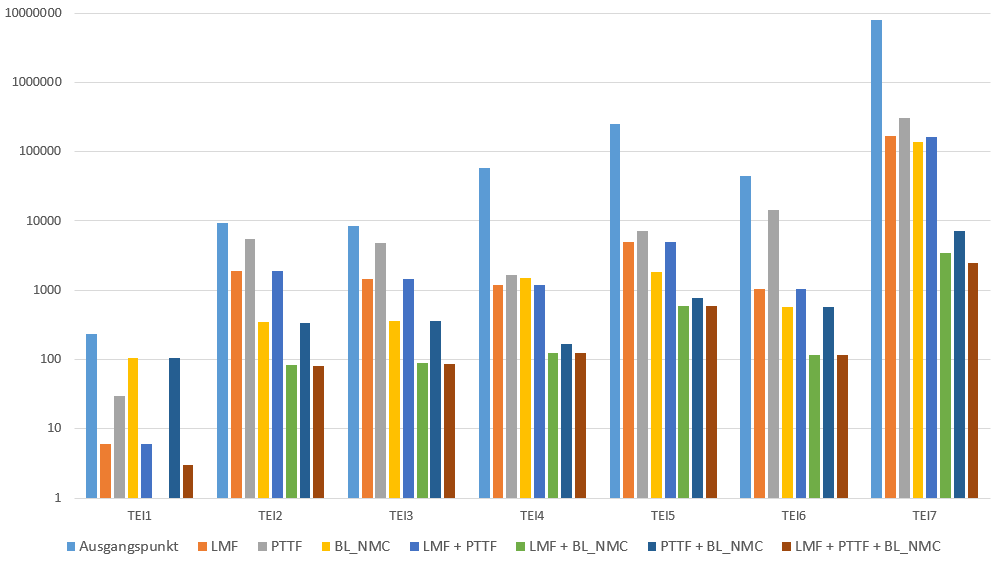
\includegraphics[width=\textwidth]{gegenueberstellung.png}
    \caption{Gegenüberstellung der Untersuchungsergebniss}
    \label{abb:gegenueberstellung}
\end{sidewaysfigure}

\chapter{Diskussion}\ref{chap_disc}
In den folgenden Abschnitten werden die Untersuchungsergebnisse aus Kapitel \ref{chap_evaluation} ausgewertet und die Vor- und Nachteile des Ansatzes zur Exploration von \emph{EJBs} zur Laufzeit gegenüber gestellt. Darüber hinaus werden Erweiterungsmöglichkeiten bzgl. der Deklaration von \emph{required Typen} und der Matcher, sowie deren zu erwartende Auswirkung auf die Exploration beschrieben. Aufbauend auf den Vor- und Nachteilen des beschriebenen Ansatzen zur testgetriebenen Evaluation von EJBs zur Laufzeit werden außerdem Erweiterungsvorschläge des Ansatzes vorgestellt.
\section{Auswertung der Untersuchungsergebnisse}
\subsection{Einzelbetrachtung}\label{disc_einzel}
Die in Kapitel \ref{chap_eval} beschriebenen Untersuchungsergebnisse zeigen, dass die Heuristiken die Anzahl der zu generierenden und zu evaluierenden Proxies reduzieren. Dabei zeigt sich, dass sich die Heuristiken nicht auf alle Explorationsdurchläufe positiv auswirken. So kann für die Heuristiken LMF und PTTF festgehalten werden, dass diese nur in den Durchlauf eine positive Wirkung erzielt, in dem ein passender Proxy auch gefunden wird.
\\\\
Die Heuristiken BL\_NMC hingegen wirkt sich auf jeden der durchgeführten Durchläufe aus. Dies liegt zu einen daran, dass die Menge der Informationen, auf deren Basis sie arbeitet, während eines Durchlaufs anwächst. Bei der Heuristik LMF ist dies nicht der Fall. Allerdings weist die Heuristik PTTF ebenfalls dieses Merkmal auf.
\\\\
Ein weiterer Grund ist, dass die Heuristik BL\_NMC dafür sorgt, dass Proxies bei der Evaluierung mitunter übersprungen werden, oder diese gar nicht erst generiert werden. Die anderen Heuristiken hingegen sorgen lediglich für eine Umsortierung der zu generierenden bzw. zu evaluierenden Proxies. Somit müssen unter der Verwendung der Heuristiken LMF und PTTF im Zweifelsfall alle Proxies generiert und erzeugt werden, auch wenn kein passender Proxy ausgemacht werden kann.
\\\\
Weiterhin ist festzuhalten, dass mit der Heuristik BL\_NMC scheinbar die besten Ergebnisse erzielt werden. Eine Ausnahme könnte hier die Exploration zum required Typ $\texttt{KOFGPCProvider}$ (\emph{TEI7}) darstellen. Die Ergebnisse bzgl. dieser Exploration sehen für die Heuristik LMF auf den ersten Blick besser aus. Allerdings konnte festgestellt werden, dass die Anzahl der Proxies, die im ersten Durchlauf im Ausgangszustand für \emph{TEI7} generiert und evaluiert werden mussten insgesamt 161294 ($\mathit{p(174)}$) beträgt. So kann festgehalten werden, dass mit der Heuristik BL\_NMC insgesamt 136141 generiert und evaluiert wurden. Damit liefert diese Heuristik die besten Ergebnisse, da die Heuristik LMF auf den ersten Durchlauf keine positive Auswirkung hat und somit in diesem 161294 Proxies generiert und evaluiert wurden.
\\\\
Bei einer Betrachtung der finalen Durchläufe - also in denen ein passender Proxy gefunden werden konnte - ergibt sich jedoch ein anderes Bild. Hierbei erweist sich in den meisten Fällen die Heuristik LMF als diejenige, mit der die besten Ergebnisse erzielt wurde. Eine Ausnahme stellen die required Typen $\texttt{FoerderprogrammeProvider}$ (\emph{TEI2}) und $\texttt{MinimalFoerderprogrammeProvider}$ (\emph{TEI3}) dar. Bei diesen beiden Typen lieferte wiederum die Heuristik BL\_NMC die besten Ergebnisse.
\\\\
Dies kann dadurch begründet werden, dass die provided Typen, die in den Methoden dieser beiden required Typen ab stärksten von denen abwichen, die in den Delegationsmethoden des passenden Proxies verwendet wurden. Aus dieser Tatsache ergibt sich für das Matcherrating ein höherer Wert, wodurch die Evaluierung des Proxies durch die Heuristik LMF weiter nach hinten verschoben wird, als es bei den Explorationen zum den übrigen required Typen der Fall war.
\subsection{Synergien}
Neben der Einzelbetrachtung der Heuristiken wurden in Abschnitt \ref{sec_kombis} auch die Kombinationen der drei Heuristiken untersucht. Aus den Feststellungen in Abschnitt \ref{disc_einzel} lässt sich ableiten, dass eine Kombinationen mit der Heuristik BL\_NMC durchaus sinnvoll ist; egal ob sie mit der Heuristik LMF oder PTTF kombiniert wird. Der Grund dafür liegt wiederum in der Tatsache, dass die Heuristiken LMF und PTTF lediglich auf einen der Explorationsdurchläufe einen positiven Effekt haben. Aus diesem Grund kann in Kombination mit der Heuristik BL\_NMC wenigstens in den anderen Durchläufen eine positive Auswirkung festgestellt werden.
\\\\
Dementgegen liefert die Kombination der Heuristiken LMF und PTTF miteinander kaum bessere Ergebnisse als die Heuristik LMF alleine. Eine Ausnahme bildet der required Typ $\texttt{KOFGPCProvider}$ (\emph{TEI7}). Dazu ist jedoch zu sagen, dass es gerade zu diesem required Typ im Vergleich zu den anderen required Typen die meisten matchenden provided Typen existieren. Insofern darf dieser scheinbare Ausreißer nicht unterschätzt werden, weshalb auch die Kombination der oben genannten Heuristiken sinnvoll ist.
\\\\
Ähnliches gilt für die Kombination aller vorgestellten Heuristiken. Dies ergibt sich jedoch ebenfalls aus den vorherigen Auswertungen bzgl. der Synergien in diesem Abschnitt. Bei der Betrachtung der Untersuchungsergebnisse zeigt sich hier ein ähnliches Muster wie zuvor: Die Kombination aller vorgestellten Heuristiken liefert nur für den required Typ $\texttt{KOFGPCProvider}$ (\emph{TEI7}) bessere Ergebnisse, als die Kombination der Heuristiken BL\_NMC und LMF. Aber auch hier darf dieses Ergebnis aufgrund der Eigenschaften von \emph{TEI7} nicht vernachlässigt werden.
\subsection{Erhöhte Komplexität}
Die vorliegende Untersuchung zweigt zwar, dass die Anzahl der zu evaluierenden Proxies in dem verwendeten System mit den vorgeschlagenen Heuristiken reduziert werden können. Allerdings wurden negative Auswirkungen wie bspw. Speichernutzung (Speicherkomplexität) oder die benötigte Zeit  (Zeitkomplexität) für die Evaluation nicht untersucht.
\\\\
Die Anwendung der Heuristiken hängt, wie in Abschnitt \ref{sec_heuristics} beschrieben, von Informationen ab, die teilweise aus den für die Proxies verwendeten \emph{provided Typen} ermittelt werden müssen (Matcherrating) bzw. nach der Ausführung der Tests über die gesamte restliche Laufzeit der Exploration verwaltet werden müssen. Von daher ist davon auszugehen, dass sich die Anwendung der Heuristiken durchaus auf den Speicherverbrauch auswirkt.
\\\\
Da die benötigte Zeit für die Verwaltung von Listen, wie sie bei den Heuristiken vorgenommen wird, mit der Anzahl der zu verwaltenden Elemente wächst, kann davon ausgegangen werden, dass die Anwendung der Heuristiken ebenfalls mehr Zeit in Anspruch nimmt, je weiter fortgeschritten die Exploration ist. Die gilt insbesondere für die Heuristiken PTTF und BL\_NMC. 
\\\\
Aufgrund dessen, dass in dieser Arbeit lediglich die Anzahl der zu evaluierenden Proxies während der Exploration untersucht wurden, ist es auch nicht auszuschließen, dass die verwendete Implementierung kein Optimierungspotential besitzt.



\section{Kritik am Ansatz}\label{sec_discApproach}

\subsection{Seiteneffekte durch Testevaluation}\label{sec_sideeffects}
Der beschriebene \emph{Explorationsprozess} erfordert die Ausführung der vordefinierten Testfälle zur Laufzeit. Sofern diese Testfälle eine Änderung des Zustands bestimmter Objekte bewirken, kann dies auch Auswirkungen auf die Funktionsweise des Systems haben. 
\\\\
Um dieses Problem zu beheben könnte sichergestellt werden, dass die Generierung der \emph{Proxies} nur auf Basis von \emph{provided Typen} (\emph{EJBs}) erfolgt, die solche Seiteneffekte nicht aufweisen. Diese Eigenschaft kann jedoch nur durch die Entwickler*innen festgestellt. Solche \emph{EJBs} können dann bspw. über Annotationen markiert werden. Während des \emph{Explorationsprozesses} könnten solche \emph{EJBs} über solche Markierungen erkannt werden. Dieser Ansatz reduziert jedoch die Anzahl der \emph{provided Typen}, die für die Generierung eines \emph{Proxies} verwendet werden können. Dadurch sinkt auch die Wahrscheinlichkeit, dass ein passender \emph{Proxy} gefunden wird.
\\\\
Um die zu markierenden \emph{EJBs} zu identifizieren ist zu prüfen, wie sich die Ausführung der einzelnen Methoden der \emph{Bean} auf das System auswirken. Es kann festgehalten werden, dass alle Methoden, die den persistenten oder den transienten Zustand von Objekten verändern, das Potential für solche unerwünschten Seiteneffekte besitzen. 
\\\\
Aufbauend auf einer solchen Prüfung einzelner Methoden, kann auch die Markierung von Methoden in Betracht gezogen werden. So dürften markierte Methoden bei der Generierung eines \emph{Proxies} nicht als \emph{Delegationsmethode} verwendet werden.
\subsection{Auswirkung auf die Verfügbarkeit eines Systems}\label{sec_stabliliy}
Die Verfügbarkeit eines Systems bzw. von Systemkomponenten, bezeichnet die Wahrscheinlichkeit, ein System oder Systemkomponenten zu einem vorgegebenen Zeitpunkt in einem funktionsfähigen Zustand anzutreffen. \cite{it-admin}
Die Auswirkung des Ansatzes auf die Verfügbarkeit wurde in dieser Arbeit nicht systematisch untersucht. Da der Ansatz jedoch darauf abzielt, bestimmte \Gls{komponente}n - in diesem Fall \emph{EJBs} - zur Laufzeit zu kombinieren, können Überlegungen bzgl. der Verfügbarkeit durchaus angestellt werden.
\\\\
Dabei muss allerdings bedacht werden, dass die Betrachtung der Verfügbarkeit einer \emph{EJB} in diesem Zusammenhang nicht ausreichend ist. Immerhin kann ein passender \emph{Proxy} auch auf einer Kombination von \emph{EJBs} erzeugt werden. Insofern bilden eher die Methoden, die von den EJBs angeboten werden, die \Gls{komponente}n in Bezug auf die oben beschriebene betrachtete Verfügbarkeit.
\\\\
Ausgehend davon kann die These aufgestellt werden, dass mit diesem Ansatz eine höhere Verfügbarkeit erreicht wird, sofern die Methoden im System redundant vorliegen. Dabei ist das Vorliegen redundanter Methoden innerhalb einer Systems wahrscheinlicher, als das Vorliegen redundanter \Gls{komponente}n, die diese Methoden enthalten\footnote{Dies ist bei \emph{EJBs} der Fall, denn eine \emph{EJB} enthält Methoden und nicht anders herum.}. 

\subsection{Auswirkung von Änderungen an bestehenden \Gls{komponente}n}
Da die \emph{EJBs} bei dem vorgestellten Ansatz nicht explizit adressiert werden, weiß der Entwickler auch nicht, an welche \emph{EJBs} die Methodenaufrufe letztendlich delegiert werden. Somit sind die Auswirkungen von Änderungen an bestehenden \Gls{komponente}n nicht direkt vorhersehbar, da sich die Menge der matchenden \emph{provided Typen} (\emph{EJBs}) und dementsprechend auch die generierten \emph{Proxies} ändern.
\\\\
Im Folgenden wird zum einen die Erweiterung um zusätzlichen \emph{provided Typen} und zum anderen die Entfernung von \emph{provided Typen} betrachtet. Dabei sei angenommen, dass die \emph{required Typen}, zu denen ein passender \emph{Proxy} gefunden werden soll, nicht verändert werden.
\subsubsection{Erweiterungen um neue \Gls{komponente}n}
Die Erweiterung von Systemen geht in Bezug auf den beschriebenen Ansatz zur testgetriebenen Exploration zur Laufzeit damit einher, dass sich die Anzahl der \emph{provided Typen} verändert. Wie in Abschnitt \ref{sec_anzahlProxies} beschrieben, besteht damit auch die Gefahr, dass die Anzahl der möglichen \emph{Proxies} steigt. Dazu muss jedoch gelten, dass eine Methode aus einem \emph{required Typ} auf eine der Methode aus dem neuen \emph{provided Typ} gematcht werden kann.
\\\\
Mehrere mögliche \emph{Proxies} haben wiederum einen Einfluss auf die Laufzeit und das Ergebnis des \emph{Explorationsprozesses}. So kann nicht davon ausgegangen werden, dass ein passender \emph{Proxy} zu einem bestimmten \emph{required Typ} genauso schnell gefunden wird, nachdem ein \emph{provided Typen} im System ergänzt wurde.
\subsubsection{Entfernen von bestehenden \Gls{komponente}n}
Ebenso wirkt sich das Entfernen eines \emph{provided Typs}, der während eines früheren \emph{Explorationsprozesses} für die Generierung eines \emph{Proxies} verwendet wurde, auf den \emph{Explorationsprozess} nach einer solchen Änderung aus. Dadurch, dass der früher verwendete \emph{provided Typ} nicht mehr vorhanden ist, muss ein anderer \emph{Proxy}, der auf andere \emph{provided Typen} basiert, erzeugt werden\footnote{sofern dies gelingt, unterstützt dies die These aus Abschnitt \ref{sec_stabliliy}}.
\\\\
Da der \emph{Explorationsprozess} beendet wird, sofern ein passender \emph{Proxy} gefunden wurde, kann es auch unter diesen Umständen dazu kommen, dass der \emph{Explorationsprozess} mitunter länger dauert als vorher. Zudem besteht in diesem Fall die Gefahr, dass während des \emph{Explorationsprozesses} kein passender \emph{Proxy} gefunden wird.

\subsection{Nutzen für den Entwickler}
Aus den vorherigen Absätzen ergibt sich, dass die Entwickler*innen bei der Verwendung dieses Ansatzes eine große Verantwortung tragen. Dieser Verantwortung können sie umso besser gerecht werden, je genauer sie das System, in dem der Ansatz verwendet werden soll, kennen. 
\\\\
So kann festgehalten werden, dass Entwickler*innen, die das System gut kennen und somit wissen, welche \Gls{komponente}n innerhalb dessen verwendet werden, diesen Ansatz wohl kaum benötigen. Vielmehr ist es ihnen möglich die passenden \Gls{komponente}n aufgrund ihres Wissens explizit zu benennen, wie es im \emph{EJB}-Framework grundlegend der Fall ist.
\\\\
Entwickler*innen, die das System hingegen weniger kennen, können von diesem Ansatz profitieren, da sie nicht selbst nach einer für ihren Anwendungsfall passenden \emph{EJB} (mitunter auch mehreren) suchen müssen. Diese können sie über die Deklaration eines \emph{required Typen} und der Spezifikation dazugehöriger Tests suchen lassen. Dabei ist jedoch zu erwähnen, dass der \emph{Explorationsprozess} insbesondere mit der vorgestellten \Gls{Heuristik} \emph{LMF} umso schneller ist, je genauer die in den Methoden des \emph{required Typs} verwendeten Typen mit den Typen, die in den Methoden der \emph{provided Typen} übereinstimmen (\emph{Matcherrating}).
\\\\
Ist den Entwickler*innen das System unbekannt, besteht die Gefahr, dass der \emph{required Typ} so deklariert wird, dass das \emph{Matcherrating} relativ hoch ausfällt und somit der \emph{Explorationsprozess} mehr Zeit in Anspruch nimmt.
\\\\
Zusammenfassend kann folgende These formuliert werden: Der Nutzen dieses Ansatzes für Entwickler*innen steht im umgekehrt proportionalen Verhältnis zum Wissen dieser Entwickler*innen über das System, in dem der Ansatz verwendet werden soll. 

\section{Erweiterungsmöglichkeiten}
\subsection{Zusätzliche Matcher}
Eine mögliche Erweiterung des Ansatzes wäre die Definition und Implementierung zusätzlicher Matcher. Diese würde es ermöglichen, dass der Abstraktionsgrad zwischen den Typen, die in den Methoden der \emph{required Typen} und \emph{provided Typen} verwendet werden, noch weiter auseinandergeht, als es bei den vorgestellten Matchern in Abschnitt \ref{sec_matcher} der Fall ist (Identität, Vererbung, Container).
\\\\
Die vorgestellten Matcher beachten beispielsweise keine impliziten Typumwandlungen (\emph{Coercions}). Diese können je nach Programmiersprache abweichen, was eine formale und allgemeine Beschreibung wie in Abschnitt \ref{sec_matcher} eines solchen Matchers (\emph{CoercionMatcher}) erschwert. So müsste ein \emph{CoercionMatcher} für jede Programmiersprache explizit spezifiziert werden.
\\\\
Die Programmiersprache Java bietet eine Vielzahl solcher impliziten Typumwandlungen an \cite{conversions_and_promotions}. Dabei ist zu beachten, dass es implizite Typumwandlungen gibt, die ohne Informationsverlust vonstatten gehen\footnote{bspw. \emph{Identity Conversion} oder \emph{Widening Primitive Conversion} \cite{conversions_and_promotions}} und solche, bei denen ein Informationsverlust nicht auszuschließen ist\footnote{bspw. \emph{Narrowing Primitive Conversion} \cite{conversions_and_promotions}}. 
\\\\
Implizite Typumwandlungen ohne Informationsverlust sind in Bezug auf die weitere Verwendung innerhalb eines \emph{Proxies} unbedenklich. Diese sind hinsichtlich des Informationsverlustes mit dem \emph{GenTypeMatcher} vergleichbar, welcher in Abschnitt \ref{sec_matcher} beschrieben wurde. So wie ein Typ $A$, der über den \emph{GenTypeMatcher} zu einem Typ $B$ gematcht wird ($B \Rightarrow_{gen} A$), ohne Probleme anstelle des Typen $B$ verwendet werden kann, kann auch ein Typ $C$, der ohne Informationsverlust implizit aus $B$ umgewandelt wurde, anstelle von $B$ verwendet werden.
\\\\
Anders ist es bei impliziten Typumwandlungen mit Informationsverlust. Diese sind eher mit dem \emph{SpecTypeMatcher} vergleichbar (siehe Abschnitt \ref{sec_matcher}). In der Spezifikation des darauf aufbauenden \emph{Proxy}-Generators ist zu erkennen, dass durch eine solche Typumwandlung bestimmte \emph{Methodendelegationen} in einen Fehler münden. Da sich der \emph{SpecTypeMatcher} direkt auf die Vererbungsbeziehung der beiden Typen bezieht, kann die Ursache solcher Fehler auf die Methoden zurückgeführt werden, die zwar im Subtyp jedoch nicht im Supertyp implementiert sind. Bei einem \emph{CoercionMatcher}, der in Abhängigkeit der Programmiersprache spezifiziert wird, kann es andere Fehlerursachen geben.
\\\\
Aus diesem Grund wäre es sinnvoll, nicht einen einzigen Matcher zu spezifizieren, der alle impliziten Typumwandlungen abdeckt. Vielmehr sollten die in der Programmiersprache definierten \emph{Coercions} nach dem möglichem Informationsverlust kategorisiert werden und dann je Kategorie ein Matcher spezifiziert werden.
\\\\
Darüber hinaus ist zu beachten, dass die Spezifikation eines Matchers alleine nicht ausreicht, um diesen zu integrieren. Da die \Gls{Heuristik} \emph{LMF} auf dem \emph{Matcherrating} aufbaut, ist es ebenso notwendig, den zusätzlichen Matchern ein Basisrating zuzuweisen. Wie in Abschnitt \ref{impl_sigma} beschrieben, wird dieses Basisrating von der Implementierung des Matchers geliefert. Dabei gilt es jedoch zu beachten, dass das Basisrating eines zusätzlichen Matchers im korrekten Verhältnis zu den bestehenden Matchern steht.
\\\\
In Bezug auf den/die \emph{CoercionMatcher} gibt es hierbei mehrere Möglichkeiten. Beispielsweise könnte für den/die \emph{CoercionMatcher} ein Basisrating zwischen 100 und 200 verwendet. Die untere Schranke von 100 wird dadurch begründet, dass es kein besseres Matching gibt, als die Identität, welche durch den \emph{ExactTypeMatcher} mit einem Basisrating von 100 beschrieben wird. Die obere Schranke von 200 könnte damit begründet werden, dass es sich um Typumwandlungen handelt, die über die Programmiersprache definiert sind und diese somit sicherer sind als ein \Gls{downcast}, der durch den \emph{SpecTypeMatcher} mit einem Basisrating von 200 abgedeckt werden.
\subsection{Default-Implementierungen in required Typen}
Im Abschnitt \ref{sec_tdcs_ejb} wurde darauf aufmerksam gemacht, dass der \emph{Explorationsprozess} das Auffinden eines passenden \emph{Proxies} nicht garantiert. Die Entwickler*innen muss also in einem solchen Fall eine alternative Implementierung bereitstellen.
\\\\
Dass ein passender \emph{Proxy} nicht gefunden wurde, kann allgemein betrachtet zwei Ursachen haben: Entweder konnte kein \emph{Proxy} generiert werden, oder keiner der generierten \emph{Proxies} erfüllt alle vordefinierten Test. 
\\\\
Die Generierung eines \emph{Proxies} hängt von dem Matching der Methoden des \emph{required Typs} und der Methoden der \emph{provided Typen} ab. Aufgrund dessen dass der Entwickler Testfälle für den \emph{required Typ} spezifizieren muss, hat er eine grundlegende Vorstellung von den Ein- und Ausgabewerten der Methoden, sowie der Verarbeitung dieser. Um nun der Gefahr vorzubeugen, dass gar kein \emph{Proxy} generiert werden kann, könnten die Entwickler*innen eine Implementierung, die seine Erwartungen zumindest minimal erfüllt, als \Gls{defaultmethode} in dem \Gls{Interface} zum \emph{required Typ} aufnehmen. Sofern bei der Exploration zu dieser Methode keine passende Methode aus einem \emph{provided Typ} gefunden wird, kann auf die Default-Implementierung zurückgegriffen werden. Der generierte \emph{Proxy}, welcher technisch gesehen das \Gls{Interface} zum \emph{required Typ} implementiert, würde den Methodenaufruf dann an sich selbst bzw. an die \Gls{defaultmethode} delegieren.
\\\\
Ein Beispiel für eine solche Konstellation zeigen die folgenden Listings. In Listing \ref{lst_calc} ist der \emph{required Typ} \emph{Calc} deklariert. Listing \ref{lst_interface_calc} zeigt das dazugehörige Java-Interface mit der \Gls{defaultmethode} $\texttt{div}$. Die Implementierung wurde so umgesetzt, dass die Testfälle, welche in der Klasse in Listing \ref{lst_testklasse_calc} enthalten sind, positiv ausfallen.
\begin{lstlisting}[caption={Required Typ \emph{Calc}},captionpos=b, style = dsl, label=lst_calc]
required Calc {
 Float div( int a, int b )	
}
\end{lstlisting}
\begin{lstlisting}[style = java, caption = Interface Calc, captionpos = b, label = lst_interface_calc]
@RequiredTypeTestReference( testClasses = CalcTest.class )
public interface Calc {

 default Float div(int a, int b){
  if(b == 0)
   return null;
  return Float.valueOf(a/b)
 }
 
}
\end{lstlisting}
\begin{lstlisting}[style = java, caption = Test CalcTest, captionpos = b, label = lst_testklasse_calc]
public class CalcTest {

 private Calc calc;
  
 @RequiredTypeInstanceSetter
 public void setProvider( Calc calc ) {
  this.calc = calc;
 }

 @RequiredTypeTest
 public void testDivByZero() {
  assertThat( calc.dev(1,0), nullValue() );
 }
  
 @RequiredTypeTest
 public void testDiv() {
  assertThat( calc.dev(4,2), equalTo(2) );
 }

}
\end{lstlisting}
\noindent
Dadurch ist zwar immer noch nicht sichergestellt, dass ein passender \emph{Proxy} in jedem Fall gefunden wird, aber den Entwickler*innen kann ein alternatives Verhalten direkt im \Gls{Interface} zum \emph{required Typ} implementieren, wodurch diese Implementierung einen sehr engen Bezug zum \emph{required Typ} hat. 


\chapter{Schlussbemerkung}\label{chap_finish}
\section{Zusammenfassung}
Zusammenfassend ist zu sagen, dass die vorgestellten \Gls{Heuristik}en ihren Zweck erfüllen und gemessen an der Anzahl der zu generierenden und zu prüfenden \emph{Proxies} eine schnellere Exploration nach einem passenden \emph{Proxy} ermöglichen. Dabei konnten auch Synergieeffekte zwischen den einzelnen \Gls{Heuristik}en festgestellt werden.
\\\\
Weiterhin wurde gezeigt, dass die testgetriebene Exploration von \emph{EJBs} zur Laufzeit grundlegend funktioniert. Dennoch gibt es Szenarien, in denen von diesem Verfahren eher abzuraten ist. Das betrifft insbesondere solche \emph{EJBs}, durch deren Methodenaufrufe eine Änderung an ihrem inneren Zustand bezweckt wird. Es wurden jedoch Möglichkeiten aufgezeigt, wie mit solchen Fällen umgegangen werden kann.
\\\\
Ob der Ansatz der testgetriebenen Exploration zur Laufzeit im Allgemeinen einen Nutzen verspricht wurde nicht geklärt. Wenn dies überhaupt der Fall ist, dann hängt der Nutzen vermutlich mit dem Wissen der Entwickler*innen zusammen, welches sie über das vorliegende System aufweisen können.
\\\\
Unabhängig davon wurde in dieser Arbeit eine allgemeine formale Beschreibung für Matcher von \Gls{wrappertype}en gegeben (\emph{ContentTypeMatcher} und \emph{ContainerTypeMatcher}). 
\\\\
Zudem können die entwickelten \Gls{Modul}e, welche in Kapitel \ref{chap_impl} beschrieben wurden, in unterschiedlichen Systemen verwendet werden. Hinsichtlich des Repositories haben die Entwickler*innen sehr viel Freiraum und sind nicht auf einen \emph{EJB-Container} beschränkt. Weiterhin können neue Matcher durch die Implementierung der dafür vorgesehenen \Gls{Interface}s in die \Gls{Modul}e integriert werden, was den Nutzen des Ansatzes in einem System individuell steigern kann.
\section{Ausblick}
Die Heuristiken wurden zwar im Rahmen der Exploration zur Laufzeit entworfen. In einem nächsten Schritt könnte versucht werden, diese Heuristiken in bestehende Search \Gls{Engine}s wie Merobase oder CodeGenie zu integriert, um so den Nutzen der Heuristiken für diese \Gls{Engine}s zu untersuchen.
\\\\
Weiterhin wäre es interessant zu untersuchen, ob und wie dieser Ansatz der Exploration von Komponenten zur Laufzeit in anderen Systemtypen wie bspw. Self-Contained-Systems funktioniert. Mitunter ergeben sich bei diesen Untersuchungen weitere Vorteile oder Probleme dieses Ansatzes.
\\\\
Darüber hinaus bieten die in Abschnitt \ref{sec_discApproach} aufgestellten Thesen bzgl. der höheren Verfügbarkeit (Abschnitt \ref{sec_sideeffects}) und dem Nutzen des Ansatzes für den Entwickler im Verhältnis zu dessen Wissen über das System das Potential für weitere Untersuchungen.


\newpage
\appendix
\addcontentsline{toc}{chapter}{Glossar}
\printglossaries

\chapter{Kombination von Matchern}\label{app_matchercombination}
Wie aus der formalen Beschreibung zum \emph{StructuralTypeMatcher} im Abschnitt \ref{subsec_structmatcher} hervorgeht, ist dieser von den übrigen Matchern abhängig. Die Implementierung der dazugehörigen Klasse $\texttt{StructuralTypeMatcher}$ verlangt zur Erzeugung eines Objektes dieser Klasse eine $\texttt{TypeMatcher}$. Dieser $\texttt{TypeMatcher}$ muss laut der formalen Beschreibung die Implementierung der Matchingrelation $\Rightarrow_{internStruct}$ darstellen.
\\\\
Zu diesem Zweck müssen die übrigen Matcher bzw. die dafür implementierten Klassen miteinander kombiniert werden, wie es in der Definition zur Matchingrelation $\Rightarrow_{internStruct}$ der Fall ist. Für solche Kombinationen steht die Klasse $\texttt{MatcherCombiner}$ im \Gls{Modul} \emph{SignatureMatching} bereit (siehe Listing \ref{lst_matchercombiner}).
\\\\
Diese Klasse erlaubt die Kombination von Objekten vom Typ $\texttt{TypeMatcher}$. 
Die Matcher-Klassen $\texttt{ExactTypeMatcher}$, $\texttt{GenSpecTypeMatcher}$ und $\texttt{WrappedTypeMatcher}$ implementieren alle dieses \Gls{Interface}. 
\\\\
Über die Methode $\texttt{combine}$ in der $\texttt{MatcherCombiner}$ wird bei der Kombination ein Supplier-Objekt erzeuge, welches über die $\texttt{get}$-Methode ein Objekt vom Typ $\texttt{TypeMatcher}$ liefern kann. Dieses $\texttt{TypeMatcher}$-Objekt versucht beim Aufruf der Methode $\texttt{matchesType(S,T)}$ die beiden Typen $S$ und $T$ über einen der kombinierten Matcher zu matchen (siehe  Listing \ref{lst_matchercombiner}). Dabei liefert die Methode $\texttt{getSortedMatcher}$ eine sortiert Liste der kombinierten Matcher. Die Sortierung wird aufsteigend entsprechend dem Basisrating (siehe auch Abschnitt \ref{sec_lmf}) der kombinierten Matcher vorgenommen .
\begin{lstlisting}[style = java, caption = Klasse: MatcherCombiner, captionpos = b, label = lst_matchercombiner]
package de.fernuni.hagen.ma.gundermann.signaturematching.matching;

import java.util.ArrayList;
import java.util.Arrays;
import java.util.Collection;
import java.util.Collections;
import java.util.List;
import java.util.function.Supplier;

import de.fernuni.hagen.ma.gundermann.signaturematching.SingleMatchingInfo;
import de.fernuni.hagen.ma.gundermann.signaturematching.matching.types.TypeMatcher;

public final class MatcherCombiner {
 private MatcherCombiner() {
 }

 public static Supplier<TypeMatcher> combine(TypeMatcher... matcher) {
  return () -> new TypeMatcher() {

   @Override
   public boolean matchesType(Class<?> checkType, Class<?> queryType) {
	for (TypeMatcher m : getSortedMatcher()) {
	 if (m.matchesType(checkType, queryType)) {
	  return true;
	 }
	}
	return false;
   }

   @Override
   public Collection<SingleMatchingInfo> calculateTypeMatchingInfos(Class<?> checkType, Class<?> queryType) {
	for (TypeMatcher m : getSortedMatcher()) {
	 if (m.matchesType(checkType, queryType)) {
	  return m.calculateTypeMatchingInfos(checkType, queryType);
	 }
	}
	return new ArrayList<>();
   }

   @Override
   public MatcherRate matchesWithRating(Class<?> checkType, Class<?> queryType) {
	for (TypeMatcher m : getSortedMatcher()) {
	 MatcherRate rating = m.matchesWithRating(checkType, queryType);
	 if (rating != null) {
	  return rating;
	 }
	}
	return null;
   }

   @Override
   public double getTypeMatcherRate() {
	// irrelevant, weil matchesWithRating ueberschrieben wurde.
	return -0;
   }

   private Collection<TypeMatcher> getSortedMatcher() {
	List<TypeMatcher> matcherList = Arrays.asList(matcher);
	Collections.sort(matcherList,(l1, l2) -> Double.compare(l1.getTypeMatcherRate(), l2.getTypeMatcherRate()));
	return matcherList;
   }

  };
 }
}
\end{lstlisting}
\noindent
Bei der Exploration wird letztendlich immer ein Objekt des der Klasse $\texttt{StructuralTypeMatcher}$ zur Ermittlung des Matchings verwendet. Listing \ref{lst_matchermanager} zeigt die Instanziierung dieses Objektes unter Verwendung der Klasse $\texttt{MatcherCombiner}$.
\begin{lstlisting}[style = java, caption = Default-Instanziierung des StructuralTypeMatchers im DesiredComponentFinder, captionpos = b, label = lst_matchermanager]
TypeMatcher exactTM = new ExactTypeMatcher();
TypeMatcher genSpecTM = new GenSpecTypeMatcher();
TypeMatcher combinedGenSpecExactTM = MatcherCombiner.combine(genSpecTM, exactTM).get();
TypeMatcher wrappedTM = new WrappedTypeMatcher(() -> combinedGenSpecExactTM);
TypeMatcher combinedWrappedGenSpecExact = MatcherCombiner.combine(genSpecTM, exactTM, wrappedTM).get();
StructuralTypeMatcher structWrappedGenSpecExactTM = new StructuralTypeMatcher(
				() -> combinedWrappedGenSpecExact);
\end{lstlisting}
\chapter{Verwendung aller Heuristiken}\label{app_semEvalMitAllenHeuristiken}
Die in den Abschnitten \ref{sec_lmf} - \ref{sec_bl_nmc} vorgestellten \Gls{Heuristik}en können miteinander kombiniert werden. Listing \ref{lst_heuristikkombination} zeigt die Implementierung der Funktionen, die für diese Kombination auf der Basis von Listing \ref{lst_semEval} angepasst oder ergänzt werden müssen.

\begin{lstlisting}[style = pseudo, caption = Kombination aller Heuristiken, captionpos = b, label = lst_heuristikkombination]
function evalProxiesMitTarget( proxies, tests ){
 testedProxies = []
 for( proxy : proxies ){
  passedTestcases = 0
  blacklistChanged = false
  evalProxy(proxy, tests)
  if( passedTests == T.size ){
   return proxy
  }
  else{
   testedProxies.add(proxy)
   if( passedTests > 0 || blacklistChanged ){
    optmizedProxies = proxies.removeAll( testedProxies )
    if( passedTests > 0 ){
     priorityTargets.addAll( proxy.targets )
     optmizedProxies = PTTF( optmizedProxies )	
    }
    if( blacklistChanged ){
     optmizedProxies = BL( optmizedProxies )	
    }
    return evalProxiesMitTarget( optmizedProxies, tests )
   }
  }
 }
 return null
}

function evalProxy(proxy, tests){
 for( test : tests ){
  try{
   if( test.eval( proxy ) ){
    passedTestcases = passedTestcases + 1
   }
   elseif( test.isSingleMethodTest ){
    methodName = test.testedSingleMethodName
    mDel = getMethodDelegation( proxy, methodName )
    methodDelegationBlacklist.add( mDel )
    blacklistChanged = true
    return
   }
  }
  catch (SigMaGlueException e){
   mDel = e.failedMethodDelegation
   methodDelegationBlacklist.add( mDel )
   blacklistChanged = true
   return
  } 
 }
}

function relevantProxies( proxies, anzahl ){
 relProxies = proxiesMitTargets( proxies, anzahl );
 optimizedLMF = LMF( relProxies )
 optimizedPTTF = PTTF( optimizedLMF )
 return BL( optimizedPTTF )
} 
\end{lstlisting}
\chapter{Deklaration der relevanten Typen}\label{app_evalTypes}
Im Folgenden erfolgt die Deklaration der \emph{required Typen}, mit denen die Evaluation der Heuristiken in Kapitel \ref{chap_evaluation} durchgeführt wird, sowie die Deklaration der \emph{provided Typen}, die als Ergebnis der jeweiligen Exploration für einen \emph{required Typ} einzeln oder in Kombination erwartet, oder innerhalb einer der Deklarationen eines \emph{required Typ} verwendet werden. Dabei ist davon auszugehen, dass diese Typen aus dem JDK als Bibliothek aufbauen.
\\\\
Die Listings \ref{lst_tei1} - \ref{lst_tei7} zeigen die Deklarationen für die \emph{required Typen}.
\begin{lstlisting}[style = dsl, caption = Deklaration von ElerFTFoerderprogrammeProvider, captionpos = b, label = lst_tei1]
required ElerFTFoerderprogrammeProvider{
	Collection getAlleFreigegebenenFPs()
	ElerFTFoerderprogramm getElerFTFoerderprogramm(DvAntragsJahr, DvFoerderprogramm, Date)
}
\end{lstlisting}
\begin{lstlisting}[style = dsl, caption = Deklaration von FoerderprogrammeProvider, captionpos = b, label = lst_tei2]
required FoerderprogrammeProvider{
	Collection getAlleFreigegebenenFPs()
	Foerderprogramm getFoerderprogramm(DvAntragsJahr, DvFoerderprogramm, Date)
}
\end{lstlisting}
\begin{lstlisting}[style = dsl, caption = Deklaration von MinimalFoerderprogrammeProvider, captionpos = b, label = lst_tei3]
required MinimalFoerderprogrammeProvider{
	Collection getAlleFreigegebenenFPs()
	Foerderprogramm getFoerderprogramm(String, int, Date)
}
\end{lstlisting}
\begin{lstlisting}[style = dsl, caption = Deklaration von IntubatingFireFighter, captionpos = b, label = lst_tei4]
required IntubatingFireFighter{
	void intubate(Injured)
	FireState extinguishFire(Fire)
}
\end{lstlisting}
\begin{lstlisting}[style = dsl, caption = Deklaration von IntubatingFreeing, captionpos = b, label = lst_tei5]
required IntubatingFreeing{
	void intubate(Injured)
	void free(Injured)
}
\end{lstlisting}
\begin{lstlisting}[style = dsl, caption = Deklaration von IntubatingPatientFireFighter, captionpos = b, label = lst_tei6]
required IntubatingFreeing{
	void intubate(IntubationPatient)
	FireState extinguishFire(Fire)
}
\end{lstlisting}
\begin{lstlisting}[style = dsl, caption = Deklaration von KOFGPCProvider, captionpos = b, label = lst_tei7]
required KOFGPCProvider{
	Collection getKOFGsVonFP(DvFoerderprogramm)
	Collection getPCsZuKOFG(DvFoerdergegenstand, DvAntragsJahr)
}
\end{lstlisting}
\noindent
Die Listings \ref{lst_ElerFTFoerderprogramm} - \ref{lst_IntubationPatient} zeigen die \emph{provided Typen}, die in den Deklarationen der \emph{required Typen} verwendet wurden und nicht Teil des JDKs sind.
\begin{lstlisting}[style = dsl, caption = Deklaration von ElerFTFoerderprogramm, captionpos = b, label = lst_ElerFTFoerderprogramm]
provided ElerFTFoerderprogramm extends Foerderprogramm{
  DvFlaeche mindestParzellenGroesse
  DvFlaeche maximaleParzellenGroesse
  int differenzKassenjahrAntragsjahr
  boolean isMehrjaehrig
  
  DvFlaeche getMaximaleParzellengroesse()
  DvFlaeche getMindestParzellenGroesse()
  int getDifferenzKassenjahrAntragsjahr()
  boolean isMehrjaehrig()
}
\end{lstlisting}
\begin{lstlisting}[style = dsl, caption = Deklaration von Foerderprogramm, captionpos = b, label = lst_Foerderprogramm]
provided Foerderprogramm extends Object{
  Long id
  STDGueltigkeit gueltigkeit
  Long fpId
  BigDecimal bagatellbetrag
  BigDecimal bagatellmenge
  List vorgaengeAm15
  Set landesmassnahmen
  
  Long getId()
  boolean isTechnischGueltig(Date)
  DvFoerderprogramm getFoerderprogramm()
  BigDecimal getBagatellmengeFoerd()
  BigDecimal getBagatellbetragFoerd()
  boolean isFachlichGueltig(DvAntragsJahr)
  STDGueltigkeit getGueltigkeit()
  Long getFpId()
}
\end{lstlisting}
%\begin{lstlisting}[style = dsl, caption = Deklartion von STDGueltigkeit, captionpos = b, label = lst_STDGueltigkeit]
%provided STDGueltigkeit extends Object{
%  STDTechnischeGueltigkeit technisch
%  STDFachlicheGueltigkeitAJ fachlich
%  STDTechnischeGueltigkeit getTechnisch()
%  STDFachlicheGueltigkeitAJ getFachlich()
%  boolean imGueltigkeitszeitraum(Date)
%  boolean imGueltigkeitszeitraum(DvAntragsJahr)
%}
%\end{lstlisting}
\begin{lstlisting}[style = dsl, caption = Deklaration von DvAntragsJahr, captionpos = b, label = lst_dvantragsjahr]
provided DvAntragsJahr extends AbstractDomainValue{
  int antragsJahr
  
  DvAntragsJahr add(int)
  int compareTo(Object)
  int intValue()
  Object readResolve()
  DvAntragsJahr getVorjahr()
  int differenz(DvAntragsJahr)
  DvAntragsJahr sub(int)
  String toStringImpl()
}
\end{lstlisting}
%\begin{lstlisting}[style = dsl, caption = Deklartion von AbstractDomainValue, captionpos = b, label = lst_AbstractDomainValue]
%provided AbstractDomainValue extends InspectableImpl{
%  boolean _isDefined
%  int compareTo(Object)
%  Object readResolve()
%  boolean isDefined()
%  void setDefined(boolean)
%  String toStringImpl()
%  String[] toStrings()
%}
%\end{lstlisting}
%\begin{lstlisting}[style = dsl, caption = Deklartion von InspectableImpl, captionpos = b, label = lst_InspectableImpl]
%provided InspectableImpl extends Object{
%  String fullAttributeName(Field)
%  boolean canWriteAttribute(String)
%  void writeAttributeValue(String, Object)
%  boolean canReadAttribute(String)
%  String[] attributeNames()
%  Object attributeValue(String)
%  Field fieldByFullName(String)
%  Field[] allFields()
%  boolean hasAttribute(String)
%}
%\end{lstlisting}
\begin{lstlisting}[style = dsl, caption = Deklaration von DvFoerderprogramm, captionpos = b, label = lst_DvFoerderprogramm]
provided DvFoerderprogramm extends DvEnumerable{
  long id
  String code
  String fpGruppe
  String bezeichnung
  String bezeichnungLang
  String getName()
  
  Long getId()
  Long getNummer()
  void validateCode(String)
  String getFpGruppe()
  String getBezeichnung()
  String toStringImpl()
  String getCode()
  String getFPNummerExtern()
  String getBezeichnungLang()
}
\end{lstlisting}
\begin{lstlisting}[style = dsl, caption = Deklaration von Injured, captionpos = b, label = lst_Injured]
provided Injured extends Object{
  Collection suffers

  Collection getSuffers()
  void healSuffer(Suffer)
  boolean isStabilized()
}
\end{lstlisting}
\begin{lstlisting}[style = dsl, caption = Deklaration von Fire, captionpos = b, label = lst_Fire]
provided Fire extends Object{
  boolean active

  void extinguish()
  boolean isActive()
}
\end{lstlisting}
\begin{lstlisting}[style = dsl, caption = Deklaration von IntubationPatient, captionpos = b, label = lst_IntubationPatient]
provided IntubationPatient extends Object{
  boolean isIntubated

  boolean isIntubated()
  void setIntubated(boolean)
}
\end{lstlisting}
\noindent
Die Listings \ref{lst_eftstd} - \ref{lst_firefighter} zeigen die Deklarationen der \emph{provided Typen}, aus denen bei der Exploration ein passender Proxy erzeugt werden soll.
\begin{lstlisting}[style = dsl, caption = Deklaration von ElerFTStammdatenAuskunftService, captionpos = b, label = lst_eftstd]
provided ElerFTStammdatenAuskunftService extends Object{
	Collection getAlleElerFTKombiKzFpFoerdergegenstaende()
	Collection getAlleElerFTKoFoerdergegenstaende()
	Collection getFeststellungscodeVerpflichtungList(FeststellungscodeVerpflichtungImplQuery)
	FeststellungscodeVerpflichtungImpl getFeststellungscodeVerpflichtungImpl(FeststellungscodeVerpflichtungImplQuery)
	Collection getAlleElerFTTierFoerdergegenstaende(DvFoerderprogramm, DvAntragsJahr, AntragsVorgangsTyp)
	Collection getAlleFreigegebenenFoerderprogramme(AntragsVorgangsTyp)
	Collection getAlleFreigegebenenFoerderprogramme()
	ElerFTKzFpFoerdergegenstand2Foerderfaehigkeit getElerFTKzFpFoerdergegenstand2Foerderfaehigkeit(DvFoerdergegenstand, DvAntragsJahr)
	FeststellungsCodeVerpflichtung2FP getFeststellungsCodeVerpflichtung2FP(FeststellungsCodeVerpflichtung2FPQuery)
	DvEftOekoFoerdergegenstandGruppe getOekoFgGruppe2Foerdergegenstand(DvFoerdergegenstand)
	Collection getAlleElerFTKzFpFoerdergegenstaende()
	VerpflichtungsGegenstandImpl getVerpflichtungsGegenstandImpl(VerpflichtungsGegenstandImplQuery)
	ElerFTVorhaben getVorhaben2Foerdergegenstand(DvFoerdergegenstand, DvAntragsJahr)
	Verpflichtungszeitraum getVerpflichtungszeitraum(DvFoerderprogramm, DvAntragsJahr)
	int getMaxStandardAnzahlZahlungen(DvFoerderprogramm, DvAntragsJahr)
	DvZusatzInfoTyp getZusatzInfo2Foerdergegenstand(DvFoerdergegenstand, DvAntragsJahr)
	int getStandardAnzahlZahlungen(DvUntermassnahme, DvAntragsJahr)
	int getStandardAnzahlZahlungen(Landesmassnahme, DvAntragsJahr)
	Collection getElerFTKoFoerdergegenstaende(DvFoerderprogramm, DvUntermassnahme, DvAntragsJahr)
	Collection getElerFTKoFoerdergegenstaende(DvFoerderprogramm)
	Collection getAlleFg2ZusatzInfo(DvZusatzInfoTyp, DvAntragsJahr)
	int getDifferenzJahrVerpflbeginnEAJ(DvFoerderprogramm, DvAntragsJahr)
	Collection getVerpflichtungsGegenstandList(VerpflichtungsGegenstandImplQuery)
	Collection getAenderungscodePropertiesList(AenderungscodePropertiesQuery)
	Collection getAlleFg2OekoFgGruppe(DvEftOekoFoerdergegenstandGruppe)
	ElerFTFoerderprogramm getFoerderprogramm(ElerFTFoerderprogrammQuery)
	ElerFTFoerderprogramm getFoerderprogramm(DvAntragsJahr, DvFoerderprogramm, Date)
	Collection getElerFTAenderung2ElerFTFP(DvFoerderprogramm)
	Collection getElerFTAenderung2ElerFTFP(ElerFTAenderung)
	ElerFTAenderung2ElerFTFP getElerFTAenderung2ElerFTFP(ElerFTAenderung, DvFoerderprogramm)
	Collection getFoerdergegenstaende(AbstractElerFTFoerdergegenstandQuery)
	Collection getElerFTTierFoerdergegenstaende(DvFoerderprogramm, DvUntermassnahme, DvAntragsJahr)
	Collection getFoerderprogramme(ElerFTFoerderprogrammQuery)
	Collection getFoerderprogramme(Date)
	Collection getAlleFoerderprogramme()
	Collection getElerFTKzFpFoerdergegenstaende(DvFoerderprogramm, DvUntermassnahme, DvAntragsJahr)
	Collection getElerFTKzFpFoerdergegenstaende(ElerFTKombiKzFpFoerdergegenstand)
	Collection getElerFTKzFpFoerdergegenstaende(DvFoerderprogramm, Finanzierungsschluessel, DvAntragsJahr)
	Collection getElerFTKzFpFoerdergegenstaende(DvFoerderprogramm, DvAntragsJahr)
	Collection getAlleFg2Vorhaben(ElerFTVorhaben, DvAntragsJahr)
	Map getKzFpJeFg(Collection, DvAntragsJahr)
}
\end{lstlisting}
\begin{lstlisting}[style = dsl, caption = Deklaration von StammdatenAuskunftService, captionpos = b, label = lst_std]
provided StammdatenAuskunftService extends Object{
  Collection getLandesmassnahmen2Foerdergegenstaende(Landesmassnahme2FoerdergegenstandQuery)
  Collection getFoerdergegenstaendeZuFinanzierungsschluessel(DvFoerderprogramm, Finanzierungsschluessel, DvAntragsJahr)
  Landesmassnahme getLandesmassnahme(Long)
  Map getOberFgJeUnterFg(DvAntragsJahr)
  Collection getFoerderprogramme(Date)
  Foerdergegenstand getFoerdergegenstand(FoerdergegenstandQuery)
  Collection getFoerdergegenstaende(DvFoerderprogramm)
  Collection getFoerdergegenstaende(FoerdergegenstandQuery)
  Collection getFoerdergegenstaende(Landesmassnahme)
  Collection getFinanzierungsschluessel(FinanzierungsschluesselQuery)
  Collection getFinanzierungskonfigurationen(FinanzierungskonfigurationQuery)
  Collection getFinanzierungskonfigurationen(Collection, DvAntragsJahr)
  Collection getFinanzierungskonfigurationen(DvAntragsJahr, DvFoerderprogramm, Long)
  Finanzierungskonfiguration getFinanzierungskonfigurationen(DvAntragsJahr, DvFoerderprogramm, DvFoerdergegenstand)
  Map getProduktcodesJeFg(DvFoerderprogramm, DvAntragsJahr, Collection, ProduktcodeArt, Finanzierungsschluessel)
  Foerderprogramm getFoerderprogramm(Foerdergegenstand)
  Foerderprogramm getFoerderprogramm(DvAntragsJahr, DvFoerderprogramm, Date)
  Collection getAblehnungsgrundCodes(Foerderprogramm, DvAntragsJahr, KuerzungsgrundCode)
  Collection getUnterFoerdergegenstaende(DvAntragsJahr, Collection)
  Collection getFoerdergegenstandGruppenZuFgs(DvAntragsJahr, Collection)
  Collection getLandesmassnahmen(DvAntragsJahr, DvFoerderprogramm)
  Collection getLandesmassnahmen(DvAntragsJahr, Foerdergegenstand)
  Collection getLandesmassnahmen(LandesmassnahmeQuery)
  Produktcode getProduktcode(ProduktcodeQuery)
  Produktcode getProduktcode(DvAntragsJahr, DvFoerdergegenstand, ProduktcodeArt)
  Produktcode getProduktcode(DvAntragsJahr, DvFoerdergegenstand, ProduktcodeArt, Finanzierungsschluessel)
  BigDecimal getBeihilfesatz(DvAntragsJahr, DvFoerdergegenstand, Integer)
  Collection getProduktcodes(DvAntragsJahr, Finanzierungsschluessel)
  Collection getProduktcodes(DvAntragsJahr, DvFoerdergegenstand, Finanzierungsschluessel)
  Collection getProduktcodes(ProduktcodeQuery)
  Collection getProduktcodes(DvAntragsJahr, DvFoerderprogramm)
  Collection getProduktcodes(DvAntragsJahr, DvFoerdergegenstand)
  Collection getProduktcodes(Collection)
  BigDecimal getKappungBetrag(DvFoerdergegenstand, DvAntragsJahr)
  Collection getVorgaenge(Date, DvFoerderprogramm)
  Collection getVorgaenge(AntragsVorgangsTyp)
  Collection getVorgaenge(Date, AntragsVorgangsTyp)
  Collection getVorgaenge()
  Collection getVorgaenge(DvFoerderprogramm, Date, AntragsVorgangsTyp)
  BigDecimal getKappungMenge(DvFoerdergegenstand, DvAntragsJahr)
  Vorgang getVorgang(DvAntragsJahr, DvFoerderprogramm, Date, AntragsVorgangsTyp, DvAntragsJahr)
  Vorgang getVorgang(DvFoerderprogramm, Date, AntragsVorgangsTyp, DvAntragsJahr)
}
\end{lstlisting}
\begin{lstlisting}[style = dsl, caption = Deklaration von Doctor, captionpos = b, label = lst_doctor]
provided Doctor extends Object{
  void provideHeartbeatMassage(Injured)
  void stablilizeBrokenBones(Injured)
  void healWithMed(Injured, Medicine)
  void placeInfusion(Injured)
  void nurseWounds(Injured)
  void intubate(Injured)
}
\end{lstlisting}
\begin{lstlisting}[style = dsl, caption = Deklaration von FireFighter, captionpos = b, label = lst_firefighter]
provided FireFighter extends Object{
  void stabilizeBrokenBones(Injured)
  void provideHeartbeatMassage(Injured)
  FireState extinguishFire(Fire)
  void free(Injured)
  void nurseWounds(Injured)
}
\end{lstlisting}
\chapter{Interfaces und Test-Implementierungen}\label{app_interfacesAndTests}
Im Folgenden werden zum einen die \Gls{Interface}s, die sich aus den Deklarationen der \emph{required Typen} aus dem Anhang \ref{app_evalTypes} ableiten lassen, aufgeführt. Zum anderen werden die Implementierungen der Testklassen, auf die die oben genannten \Gls{Interface}s über die Annotation $\texttt{RequiredTypeTestReference}$ verweisen, dargelegt. 
\\\\
Die Listings \ref{lst_interfaces_tei1} - \ref{lst_interfaces_tei7} zeigen dabei die Deklarationen der Java-Interfaces\footnote{Auf die Import-Anweisungen wurde verzichtet.} für die \emph{required Typen} aus Tabelle \ref{tab:eIShort} aus Kapitel \ref{chap_evaluation}.
\begin{lstlisting}[style = java, caption = Interface ElerFTFoerderprogrammeProvider, captionpos = b, label = lst_interfaces_tei1]
@RequiredTypeTestReference( testClasses = ElerFTFoerderprogrammProviderTest.class )
public interface ElerFTFoerderprogrammeProvider {

  Collection<ElerFTFoerderprogramm> getAlleFreigegebenenFPs();

  ElerFTFoerderprogramm getElerFTFoerderprogramm( DvAntragsJahr jahr, DvFoerderprogramm fp, Date date );
  
}
\end{lstlisting}
\begin{lstlisting}[style = java, caption = Interface FoerderprogrammeProvider, captionpos = b, label = lst_interfaces_tei2]
@RequiredTypeTestReference( testClasses = FoerderprogrammProviderTest.class )
public interface FoerderprogrammeProvider {

 Collection<Foerderprogramm> getAlleFreigegebenenFPs();

   Foerderprogramm getFoerderprogramm( DvFoerderprogramm fp, DvAntragsJahr jahr, Date date );
   
}
\end{lstlisting}
\begin{lstlisting}[style = java, caption = Interface MinimalFoerderprogrammeProvider, captionpos = b, label = lst_interfaces_tei3]
@RequiredTypeTestReference( testClasses = MinimalFoerderprogrammProviderTest.class )
public interface MinimalFoerderprogrammeProvider {

  Collection<String> getAlleFreigegebenenFPs();

  Foerderprogramm getFoerderprogramm( String fp, int jahr, Date date );
  
}
\end{lstlisting}
\begin{lstlisting}[style = java, caption = Interface IntubatingFireFighter, captionpos = b, label = lst_interfaces_tei4]
@RequiredTypeTestReference( testClasses = IntubatingFireFighterTest.class )
public interface IntubatingFireFighter {

  public void intubate( Injured injured );

  public FireState extinguishFire( Fire fire );
  
}
\end{lstlisting}
\begin{lstlisting}[style = java, caption = Interface IntubatingFreeing, captionpos = b, label = lst_interfaces_tei5]
@RequiredTypeTestReference( testClasses = IntubatingFreeingTest.class )
public interface IntubatingFreeing {

  public void intubate( Injured injured );

  public void free( Injured injured );
  
}
\end{lstlisting}
\begin{lstlisting}[style = java, caption = Interface IntubatingPatientFireFighter, captionpos = b, label = lst_interfaces_tei6]
@RequiredTypeTestReference( testClasses = IntubatingPatientFireFighterTest.class )
public interface IntubatingPatientFireFighter {

  public void intubate( IntubationPartient patient );

  public FireState extinguishFire( Fire fire );
  
}
\end{lstlisting}
\begin{lstlisting}[style = java, caption = Interface KOFGPCProvider, captionpos = b, label = lst_interfaces_tei7]
@RequiredTypeTestReference( testClasses = KOFGPCProviderTest.class )
public interface KOFGPCProvider {

  Collection<ElerFTKoFoerdergegenstand> getKOFGsVonFP( DvFoerderprogramm fp );
 
  Collection<Produktcode> getPCsZuKOFG( DvFoerdergegenstand fg, DvAntragsJahr aj ); 
  
}
\end{lstlisting}
Zu erkennen ist, dass jedes \Gls{Interface}s, wie in Abschnitt \ref{sec_Impl_CT} beschrieben, mit der Annotation $\texttt{RequiredTypeTestReference}$ versehen ist, über die auf eine Java-Klasse verwiesen wird, in der die Tests zu dem jeweiligen \emph{required Typ} implementiert sind.
\\\\
Die Listings \ref{lst_testklassen_tei1} - \ref{lst_testklassen_tei7} zeigen die Implementierungen dieser Testklassen\footnote{Auf die Import-Anweisungen wurde verzichtet.}.
\begin{lstlisting}[style = java, caption = Interface ElerFTFoerderprogrammProviderTest, captionpos = b, label = lst_testklassen_tei1]
public class ElerFTFoerderprogrammProviderTest implements TriedMethodCallsInfo {

  private ElerFTFoerderprogrammeProvider provider;
  private Collection<Method> calledMethods = new ArrayList<Method>();
  
  @RequiredTypeInstanceSetter
  public void setProvider( ElerFTFoerderprogrammeProvider provider ) {
    this.provider = provider;
  }

  @RequiredTypeTest
  public void testEmptyCollection() {
    addTriedMethodCall( getMethod( "getAlleFreigegebenenFPs", ElerFTFoerderprogrammeProvider.class ) );
    Collection<ElerFTFoerderprogramm> alleFreigegebenenFPs = provider.getAlleFreigegebenenFPs();
    assertThat( alleFreigegebenenFPs, notNullValue() );
  }

  @RequiredTypeTest
  public void testMockedFPCollection() {
    DvFoerderprogramm fp = DvFoerderprogramm.Factory.valueOf( DvFoerderprogramm.FP215 );
    addTriedMethodCall( getMethod( "getElerFTFoerderprogramm", ElerFTFoerderprogrammeProvider.class ) );
    ElerFTFoerderprogramm alleFreigegebenenFPs = provider.getElerFTFoerderprogramm( DvAntragsJahr.AJ2020,
        fp, new Date() );
    assertThat( alleFreigegebenenFPs, nullValue() );
  }

  @Override
  public void addTriedMethodCall( Method method ) {
    calledMethods.add( method );
  }

  @Override
  public Collection<Method> getTriedMethodCalls() {
    return calledMethods;
  }

}
\end{lstlisting}
\begin{lstlisting}[style = java, caption = Interface FoerderprogrammProviderTest, captionpos = b, label = lst_testklassen_tei2]
public class FoerderprogrammProviderTest implements TriedMethodCallsInfo {

  private FoerderprogrammeProvider provider;

  private Collection<Method> calledMethods = new ArrayList<Method>();

  @RequiredTypeInstanceSetter
  public void setProvider( FoerderprogrammeProvider provider ) {
    this.provider = provider;
  }

  @RequiredTypeTest
  public void testEmptyCollection() {
    addTriedMethodCall( getMethod( "getAlleFreigegebenenFPs", FoerderprogrammeProvider.class ) );
    Collection<Foerderprogramm> alleFreigegebenenFPs = provider.getAlleFreigegebenenFPs();
    assertThat( alleFreigegebenenFPs, notNullValue() );
  }

  @RequiredTypeTest
  public void testMockedFPCollection() {
    DvFoerderprogramm fp = DvFoerderprogramm.Factory.valueOf( DvFoerderprogramm.FP508 );
    addTriedMethodCall( getMethod( "getFoerderprogramm", FoerderprogrammeProvider.class ) );
    Foerderprogramm relevantFP = provider.getFoerderprogramm( fp, DvAntragsJahr.AJ2020,
        new Date() );
    assertThat( relevantFP, notNullValue() );
  }

  @RequiredTypeTest
  public void testDZFPCollection() {
    DvFoerderprogramm fp = DvFoerderprogramm.Factory.valueOf( DvFoerderprogramm.FP215 );
    addTriedMethodCall( getMethod( "getFoerderprogramm", FoerderprogrammeProvider.class ) );
    Foerderprogramm relevantFP = provider.getFoerderprogramm( fp, DvAntragsJahr.AJ2020,
        new Date() );
    assertThat( relevantFP, notNullValue() );
  }

  @Override
  public void addTriedMethodCall( Method method ) {
    calledMethods.add( method );
  }

  @Override
  public Collection<Method> getTriedMethodCalls() {
    return calledMethods;
  }

}
\end{lstlisting}
\begin{lstlisting}[style = java, caption = Interface MinimalFoerderprogrammProviderTest, captionpos = b, label = lst_testklassen_tei3]
public class MinimalFoerderprogrammProviderTest implements TriedMethodCallsInfo {

  private MinimalFoerderprogrammeProvider provider;
  private Collection<Method> calledMethods = new ArrayList<Method>();

  @RequiredTypeInstanceSetter
  public void setProvider( MinimalFoerderprogrammeProvider provider ) {
    this.provider = provider;
  }

  @RequiredTypeTest
  public void testEmptyCollection() {
    addTriedMethodCall( getMethod( "getAlleFreigegebenenFPs", MinimalFoerderprogrammeProvider.class) );
    Collection<String> alleFreigegebenenFPs = provider.getAlleFreigegebenenFPs();
    assertThat( alleFreigegebenenFPs, notNullValue() );
  }

  @RequiredTypeTest
  public void testGetFoerderprogramm() {
    String fpCode = "215";
    addTriedMethodCall( getMethod( "getFoerderprogramm", MinimalFoerderprogrammeProvider.class) );
    Foerderprogramm fp = provider.getFoerderprogramm( fpCode, 2015, new Date() );
    assertThat( fp, notNullValue() );
    DvFoerderprogramm dvFP = fp.getFoerderprogramm();
    assertThat( dvFP, notNullValue() );

    String code = dvFP.getCode();
    assertThat( fpCode, equalTo( code ) );

  }

  @Override
  public void addTriedMethodCall( Method method ) {
    calledMethods.add( method );
  }

  @Override
  public Collection<Method> getTriedMethodCalls() {
    return calledMethods ;
  }

}
\end{lstlisting}
\begin{lstlisting}[style = java, caption = Interface IntubatingFireFighterTest, captionpos = b, label = lst_testklassen_tei4]
public class IntubatingFireFighterTest implements TriedMethodCallsInfo {

	private IntubatingFireFighter intubatingFireFighter;
	private Collection<Method> calledMethods = new ArrayList<Method>();

	@RequiredTypeInstanceSetter
	public void setProvider(IntubatingFireFighter intubatingFireFighter) {
		this.intubatingFireFighter = intubatingFireFighter;
	}

	@RequiredTypeTest
	public void free() {
		Fire fire = new Fire();
		addTriedMethodCall(getMethod("extinguishFire", IntubatingFireFighter.class));
		FireState fireState = intubatingFireFighter.extinguishFire(fire);
		assertTrue(Objects.equals(fireState.isActive(), fire.isActive()));
		assertFalse(fire.isActive());
	}

	@RequiredTypeTest
	public void intubate() {
		Collection<Suffer> suffer = Arrays.asList(Suffer.BREATH_PROBLEMS);
		Injured patient = new Injured(suffer);
		addTriedMethodCall(getMethod("intubate", IntubatingFireFighter.class));
		intubatingFireFighter.intubate(patient);
		assertTrue(patient.isStabilized());
	}

	@Override
	public void addTriedMethodCall(Method m) {
		calledMethods.add(m);
	}

	@Override
	public Collection<Method> getTriedMethodCalls() {
		return calledMethods;
	}

}
\end{lstlisting}
\begin{lstlisting}[style = java, caption = Interface IntubatingFreeingTest, captionpos = b, label = lst_testklassen_tei5]
public class IntubatingFreeingTest implements TriedMethodCallsInfo {

	private IntubatingFreeing intubatingFreeing;
	private Collection<Method> calledMethods = new ArrayList<Method>();

	@RequiredTypeInstanceSetter
	public void setProvider(IntubatingFreeing intubatingFireFighter) {
		this.intubatingFreeing = intubatingFireFighter;
	}

	@RequiredTypeTest
	public void free() {
		Collection<Suffer> suffer = Arrays.asList(Suffer.LOCKED);
		Injured patient = new Injured(suffer);
		addTriedMethodCall(getMethod("free", IntubatingFreeing.class));
		intubatingFreeing.free(patient);
		assertTrue(patient.isStabilized());
	}

	@RequiredTypeTest
	public void intubate() {
		Collection<Suffer> suffer = Arrays.asList(Suffer.BREATH_PROBLEMS);
		Injured patient = new Injured(suffer);
		addTriedMethodCall(getMethod("intubate", IntubatingFreeing.class));
		intubatingFreeing.intubate(patient);
		assertTrue(patient.isStabilized());
	}

	@Override
	public void addTriedMethodCall(Method m) {
		calledMethods.add(m);
	}

	@Override
	public Collection<Method> getTriedMethodCalls() {
		return calledMethods;
	}
	
}
\end{lstlisting}
\begin{lstlisting}[style = java, caption = Interface IntubatingPatientFireFighterTest, captionpos = b, label = lst_testklassen_tei6]
public class IntubatingPatientFireFighterTest implements TriedMethodCallsInfo {

	private IntubatingPatientFireFighter intubatingPatientFireFighter;
	private Collection<Method> calledMethods = new ArrayList<Method>();

	@RequiredTypeInstanceSetter
	public void setProvider(IntubatingPatientFireFighter intubatingFireFighter) {
		this.intubatingPatientFireFighter = intubatingFireFighter;
	}

	@RequiredTypeTest
	public void extinguishFire() {
		Fire fire = new Fire();
		addTriedMethodCall(getMethod("extinguishFire", IntubatingPatientFireFighter.class));
		FireState fireState = intubatingPatientFireFighter.extinguishFire(fire);
		assertTrue(Objects.equals(fireState.isActive(), fire.isActive()));
		assertFalse(fire.isActive());
	}

	@RequiredTypeTest
	public void intubate() {
		IntubationPartient patient = new IntubationPartient();
		addTriedMethodCall(getMethod("intubate", IntubatingPatientFireFighter.class));
		intubatingPatientFireFighter.intubate(patient);
		assertTrue(patient.isIntubated());
	}

	@Override
	public void addTriedMethodCall(Method m) {
		calledMethods.add(m);
	}

	@Override
	public Collection<Method> getTriedMethodCalls() {
		return calledMethods;
	}

}
\end{lstlisting}
\begin{lstlisting}[style = java, caption = Interface KOFGPCProviderTest, captionpos = b, label = lst_testklassen_tei7]
public class KOFGPCProviderTest implements TriedMethodCallsInfo {

  private KOFGPCProvider provider;

  private Collection<Method> calledMethods = new ArrayList<Method>();

  @RequiredTypeInstanceSetter
  public void setProvider( KOFGPCProvider provider ) {
    this.provider = provider;
  }

  @RequiredTypeTest
  public void testKOFGsCollection() {
    DvFoerderprogramm fp = DvFoerderprogramm.Factory.valueOf( DvFoerderprogramm.FP508 );
    addTriedMethodCall( getMethod( "getKOFGsVonFP", KOFGPCProvider.class ) );
    Collection<ElerFTKoFoerdergegenstand> kofGsVonFP = provider.getKOFGsVonFP( fp );
    assertThat( kofGsVonFP, notNullValue() );
    assertThat( kofGsVonFP.isEmpty(), equalTo( false ) );
    assertThat( kofGsVonFP.stream().anyMatch( fg -> fg.getCode().equals( "KO508" ) ), equalTo( true ) );
  }

  @RequiredTypeTest
  public void testPCsCollection() {
    DvFoerdergegenstand fg = DvFoerdergegenstand.Factory.valueOf( 20155080025L );
    addTriedMethodCall( getMethod( "getPCsZuKOFG", KOFGPCProvider.class ) );
    Collection<Produktcode> pcs = provider.getPCsZuKOFG( fg, DvAntragsJahr.AJ2020 );
    assertThat( pcs, notNullValue() );
    assertThat( pcs.isEmpty(), equalTo( false ) );
  }

  @Override
  public void addTriedMethodCall( Method m ) {
    this.calledMethods.add( m );
  }

  @Override
  public Collection<Method> getTriedMethodCalls() {
    return calledMethods;
  }

}
\end{lstlisting}
\noindent
Hier ist zu erkennen, dass die Testklassen alle das \Gls{Interface}s $\texttt{TriedMethodCallsInfo}$ implementieren, über das die für die Heuristik \emph{BL\_NMC} benötigten Informationen (siehe Abschnitt \ref{sec_bl_nmc}) ermittelt werden. Ebenso ist die Implementierung dieses \Gls{Interface}s in den oben genannten Listings zu erkennen.
\chapter{Ergebnisse für die Heuristik LMF (Ergänzungen)}\label{app_matcherratingEval}
In diesem Abschnitt werden die Untersuchungsergebnisse der Heuristik \emph{LMF} mit allen Varianten zur Bestimmung des Matcherratings aus Abschnitt \ref{sec_lmf} dargelegt. Dieses Kapitel bildet somit eine Ergänzung zu Abschnitt \ref{sec_evalLMF}. Die darin beschriebenen Ergebnisse der Variante \emph{1.1} werden der Vollständigkeit halber in dem vorliegenden Kapitel nochmals aufgeführt.
\\\\
Die folgenden Ergebnisse beziehen sich auf die in Kapitel \ref{chap_evaluation} vorgestellten \emph{required Typen} \emph{TEI1}-\emph{TEI7}.
\pagebreak
\section{Ergebnisse für Variante 1.1}
\begin{multicols}{3}
\vft{1}{5}{$p(44)-6$}{1}{0}{Ergebnisse \emph{LMF} mit Variante 1.1 für TEI1 1.~\mbox{Durchlauf}}{lmf11_TEI1_1_app}
\vft{1}{1889}{$p(55)-1890$}{1}{0}{Ergebnisse \emph{LMF} mit Variante 1.1 für TEI2 1.~\mbox{Durchlauf}}{lmf11_TEI2_1_app}
\vft{1}{1463}{$p(50)-1464$}{1}{0}{Ergebnisse \emph{LMF} mit Variante 1.1 für TEI3 1.~\mbox{Durchlauf}}{lmf11_TEI3_1_app}
\end{multicols}

\begin{multicols}{2}
\vft{1}{$1174$}{0}{0}{0}{Ergebnisse \emph{LMF} mit Variante 1.1 für TEI4 1. Durchlauf}{lmf11_TEI4_1_app}
\vft{2}{2}{$p(2247)-3$}{1}{0}{Ergebnisse \emph{LMF} mit Variante 1.1 für TEI4 2. Durchlauf}{lmf11_TEI4_2_app}
\end{multicols}
\begin{multicols}{2}
\vft{1}{$4984$}{0}{0}{0}{Ergebnisse \emph{LMF} mit Variante 1.1 für TEI5 1. Durchlauf}{lmf11_TEI5_1_app}
\vft{2}{32}{$p(2775)-33$}{1}{0}{Ergebnisse \emph{LMF} mit Variante 1.1 für TEI5 2. Durchlauf}{lmf11_TEI5_2_app}
\end{multicols}
\begin{multicols}{2}
\vft{1}{$1051$}{0}{0}{0}{Ergebnisse \emph{LMF} mit Variante 1.1 für TEI6 1. Durchlauf}{lmf11_TEI6_1_app}
\vft{2}{0}{$p(1323)-1$}{1}{0}{Ergebnisse \emph{LMF} mit Variante 1.1 für TEI6 2. Durchlauf}{lmf11_TEI6_2_app}
\end{multicols}
\begin{multicols}{2}
\vft{1}{$161294$}{0}{0}{0}{Ergebnisse \emph{LMF} mit Variante 1.1 für TEI7 1. Durchlauf}{lmf11_TEI7_1_app}
\vft{2}{7641}{$p(52150)-7642$}{1}{0}{Ergebnisse \emph{LMF} mit Variante 1.1 für TEI7 2. Durchlauf}{lmf11_TEI7_2_app}
\end{multicols}
\section{Ergebnisse für Variante 1.2}
\begin{multicols}{3}
\vft{1}{1}{$p(44)-2$}{1}{0}{Ergebnisse \emph{LMF} mit Variante 1.2 für TEI1 1.~\mbox{Durchlauf}}{lmf12_TEI1_1}
\vft{1}{2783}{$p(55)-2784$}{1}{0}{Ergebnisse \emph{LMF} mit Variante 1.2 für TEI2 1.~\mbox{Durchlauf}}{lmf12_TEI2_1}
\vft{1}{1830}{$p(50)-1831$}{1}{0}{Ergebnisse \emph{LMF} mit Variante 1.2 für TEI3 1.~\mbox{Durchlauf}}{lmf12_TEI3_1}
\end{multicols}
\begin{multicols}{2}
\vft{1}{$1174$}{0}{0}{0}{Ergebnisse \emph{LMF} mit Variante 1.2 für TEI4 1. Durchlauf}{lmf12_TEI4_1}
\vft{2}{3}{$p(2247)-4$}{1}{0}{Ergebnisse \emph{LMF} mit Variante 1.2 für TEI4 2. Durchlauf}{lmf12_TEI4_2}
\end{multicols}
\begin{multicols}{2}
\vft{1}{$4984$}{0}{0}{0}{Ergebnisse \emph{LMF} mit Variante 1.2 für TEI5 1. Durchlauf}{lmf12_TEI5_1}
\vft{2}{3}{$p(2775)-4$}{1}{0}{Ergebnisse \emph{LMF} mit Variante 1.2 für TEI5 2. Durchlauf}{lmf12_TEI5_2}
\end{multicols}

\begin{multicols}{2}
\vft{1}{$1051$}{0}{0}{0}{Ergebnisse \emph{LMF} mit Variante 1.2 für TEI6 1. Durchlauf}{lmf12_TEI6_1}
\vft{2}{0}{$p(1323)-1$}{1}{0}{Ergebnisse \emph{LMF} mit Variante 1.2 für TEI6 2. Durchlauf}{lmf12_TEI6_2}
\end{multicols}
\pagebreak
\begin{multicols}{2}
\vft{1}{$161294$}{0}{0}{0}{Ergebnisse \emph{LMF} mit Variante 1.2 für TEI7 1. Durchlauf}{lmf12_TEI7_1}
\vft{2}{161298}{$p(52150)-161299$}{1}{0}{Ergebnisse \emph{LMF} mit Variante 1.2 für TEI7 2. Durchlauf}{lmf12_TEI7_2}
\end{multicols}
\section{Ergebnisse für Variante 1.3}
\begin{multicols}{3}
\vft{1}{50}{$p(44)-51$}{1}{0}{Ergebnisse \emph{LMF} mit Variante 1.3 für TEI1 1.~\mbox{Durchlauf}}{lmf13_TEI1_1}
\vft{1}{20}{$p(55)-21$}{1}{0}{Ergebnisse \emph{LMF} mit Variante 1.3 für TEI2 1.~\mbox{Durchlauf}}{lmf13_TEI2_1}
\vft{1}{121}{$p(50)-122$}{1}{0}{Ergebnisse \emph{LMF} mit Variante 1.3 für TEI3 1.~\mbox{Durchlauf}}{lmf13_TEI3_1}
\end{multicols}
\begin{multicols}{2}
\vft{1}{$1174$}{0}{0}{0}{Ergebnisse \emph{LMF} mit Variante 1.3 für TEI4 1. Durchlauf}{lmf13_TEI4_1}
\vft{2}{57}{$p(2247)-58$}{1}{0}{Ergebnisse \emph{LMF} mit Variante 1.3 für TEI4 2. Durchlauf}{lmf13_TEI4_2}
\end{multicols}
\begin{multicols}{2}
\vft{1}{$4984$}{0}{0}{0}{Ergebnisse \emph{LMF} mit Variante 1.3 für TEI5 1. Durchlauf}{lmf13_TEI5_1}
\vft{2}{6246}{$p(2775)-6247$}{1}{0}{Ergebnisse \emph{LMF} mit Variante 1.3 für TEI5 2. Durchlauf}{lmf13_TEI5_2}
\end{multicols}

\begin{multicols}{2}
\vft{1}{$1051$}{0}{0}{0}{Ergebnisse \emph{LMF} mit Variante 1.3 für TEI6 1. Durchlauf}{lmf13_TEI6_1}
\vft{2}{5}{$p(1323)-6$}{1}{0}{Ergebnisse \emph{LMF} mit Variante 1.3 für TEI6 2. Durchlauf}{lmf13_TEI6_2}
\end{multicols}

\begin{multicols}{2}
\vft{1}{$161294$}{0}{0}{0}{Ergebnisse \emph{LMF} mit Variante 1.3 für TEI7 1. Durchlauf}{lmf13_TEI7_1}
\vft{2}{121074}{$p(52150)-121075$}{1}{0}{Ergebnisse \emph{LMF} mit Variante 1.3 für TEI7 2. Durchlauf}{lmf13_TEI7_2}
\end{multicols}

\section{Ergebnisse für Variante 1.4}
\begin{multicols}{3}
\vft{1}{45}{$p(44)-46$}{1}{0}{Ergebnisse \emph{LMF} mit Variante 1.4 für TEI1 1.~\mbox{Durchlauf}}{lmf14_TEI1_1}
\vft{1}{2025}{$p(55)-2026$}{1}{0}{Ergebnisse \emph{LMF} mit Variante 1.4 für TEI2 1.~\mbox{Durchlauf}}{lmf14_TEI2_1}
\vft{1}{1517}{$p(50)-1518$}{1}{0}{Ergebnisse \emph{LMF} mit Variante 1.4 für TEI3 1.~\mbox{Durchlauf}}{lmf14_TEI3_1}
\end{multicols}
\begin{multicols}{2}
\vft{1}{$1174$}{0}{0}{0}{Ergebnisse \emph{LMF} mit Variante 1.4 für TEI4 1. Durchlauf}{lmf14_TEI4_1}
\vft{2}{4}{$p(2247)-5$}{1}{0}{Ergebnisse \emph{LMF} mit Variante 1.4 für TEI4 2. Durchlauf}{lmf14_TEI4_2}
\end{multicols}
\begin{multicols}{2}
\vft{1}{$4984$}{0}{0}{0}{Ergebnisse \emph{LMF} mit Variante 1.4 für TEI5 1. Durchlauf}{lmf14_TEI5_1}
\vft{2}{34}{$p(2775)-35$}{1}{0}{Ergebnisse \emph{LMF} mit Variante 1.4 für TEI5 2. Durchlauf}{lmf14_TEI5_2}
\end{multicols}

\begin{multicols}{2}
\vft{1}{$1051$}{0}{0}{0}{Ergebnisse \emph{LMF} mit Variante 1.4 für TEI6 1. Durchlauf}{lmf14_TEI6_1}
\vft{2}{0}{$p(1323)-1$}{1}{0}{Ergebnisse \emph{LMF} mit Variante 1.4 für TEI6 2. Durchlauf}{lmf14_TEI6_2}
\end{multicols}

\begin{multicols}{2}
\vft{1}{$161294$}{0}{0}{0}{Ergebnisse \emph{LMF} mit Variante 1.4 für TEI7 1. Durchlauf}{lmf14_TEI7_1}
\vft{2}{21068}{$p(52150)-21069$}{1}{0}{Ergebnisse \emph{LMF} mit Variante 1.4 für TEI7 2. Durchlauf}{lmf14_TEI7_2}
\end{multicols}

\section{Ergebnisse für Variante 2.1}
\begin{multicols}{3}
\vft{1}{8}{$p(44)-9$}{1}{0}{Ergebnisse \emph{LMF} mit Variante 2.1 für TEI1 1.~\mbox{Durchlauf}}{lmf21_TEI1_1}
\vft{1}{3975}{$p(55)-3976$}{1}{0}{Ergebnisse \emph{LMF} mit Variante 2.1 für TEI2 1.~\mbox{Durchlauf}}{lmf21_TEI2_1}
\vft{1}{2933}{$p(50)-2934$}{1}{0}{Ergebnisse \emph{LMF} mit Variante 2.1 für TEI3 1.~\mbox{Durchlauf}}{lmf21_TEI3_1}
\end{multicols}
\begin{multicols}{2}
\vft{1}{$1174$}{0}{0}{0}{Ergebnisse \emph{LMF} mit Variante 2.1 für TEI4 1. Durchlauf}{lmf21_TEI4_1}
\vft{2}{2}{$p(2247)-3$}{1}{0}{Ergebnisse \emph{LMF} mit Variante 2.1 für TEI4 2. Durchlauf}{lmf21_TEI4_2}
\end{multicols}
\begin{multicols}{2}
\vft{1}{$4984$}{0}{0}{0}{Ergebnisse \emph{LMF} mit Variante 2.1 für TEI5 1. Durchlauf}{lmf21_TEI5_1}
\vft{2}{32}{$p(2775)-33$}{1}{0}{Ergebnisse \emph{LMF} mit Variante 2.1 für TEI5 2. Durchlauf}{lmf21_TEI5_2}
\end{multicols}

\begin{multicols}{2}
\vft{1}{$1051$}{0}{0}{0}{Ergebnisse \emph{LMF} mit Variante 2.1 für TEI6 1. Durchlauf}{lmf21_TEI6_1}
\vft{2}{0}{$p(1323)-1$}{1}{0}{Ergebnisse \emph{LMF} mit Variante 2.1 für TEI6 2. Durchlauf}{lmf21_TEI6_2}
\end{multicols}

\begin{multicols}{2}
\vft{1}{$161294$}{0}{0}{0}{Ergebnisse \emph{LMF} mit Variante 2.1 für TEI7 1. Durchlauf}{lmf21_TEI7_1}
\vft{2}{32018037}{$p(52150)-32018038$}{1}{0}{Ergebnisse \emph{LMF} mit Variante 2.1 für TEI7 2. Durchlauf}{lmf21_TEI7_2}
\end{multicols}

\section{Ergebnisse für Variante 2.2}
\begin{multicols}{3}
\vft{1}{0}{$p(44)-1$}{1}{0}{Ergebnisse \emph{LMF} mit Variante 2.2 für TEI1 1.~\mbox{Durchlauf}}{lmf22_TEI1_1}
\vft{1}{8007}{$p(55)-8008$}{1}{0}{Ergebnisse \emph{LMF} mit Variante 2.2 für TEI2 1.~\mbox{Durchlauf}}{lmf22_TEI2_1}
\vft{1}{7104}{$p(50)-7105$}{1}{0}{Ergebnisse \emph{LMF} mit Variante 2.2 für TEI3 1.~\mbox{Durchlauf}}{lmf22_TEI3_1}
\end{multicols}
\begin{multicols}{2}
\vft{1}{$1174$}{0}{0}{0}{Ergebnisse \emph{LMF} mit Variante 2.2 für TEI4 1. Durchlauf}{lmf22_TEI4_1}
\vft{2}{0}{$p(2247)-1$}{1}{0}{Ergebnisse \emph{LMF} mit Variante 2.2 für TEI4 2. Durchlauf}{lmf22_TEI4_2}
\end{multicols}
\begin{multicols}{2}
\vft{1}{$4984$}{0}{0}{0}{Ergebnisse \emph{LMF} mit Variante 2.2 für TEI5 1. Durchlauf}{lmf22_TEI5_1}
\vft{2}{0}{$p(2775)-1$}{1}{0}{Ergebnisse \emph{LMF} mit Variante 2.2 für TEI5 2. Durchlauf}{lmf22_TEI5_2}
\end{multicols}

\begin{multicols}{2}
\vft{1}{$1051$}{0}{0}{0}{Ergebnisse \emph{LMF} mit Variante 2.2 für TEI6 1. Durchlauf}{lmf22_TEI6_1}
\vft{2}{0}{$p(1323)-1$}{1}{0}{Ergebnisse \emph{LMF} mit Variante 2.2 für TEI6 2. Durchlauf}{lmf22_TEI6_2}
\end{multicols}

\begin{multicols}{2}
\vft{1}{$161294$}{0}{0}{0}{Ergebnisse \emph{LMF} mit Variante 2.2 für TEI7 1. Durchlauf}{lmf22_TEI7_1}
\vft{2}{2840500}{$p(52150)-2840501$}{1}{0}{Ergebnisse \emph{LMF} mit Variante 2.2 für TEI7 2. Durchlauf}{lmf22_TEI7_2}
\end{multicols}

\section{Ergebnisse für Variante 2.3}
\begin{multicols}{3}
\vft{1}{5}{$p(44)-6$}{1}{0}{Ergebnisse \emph{LMF} mit Variante 2.3 für TEI1 1.~\mbox{Durchlauf}}{lmf23_TEI1_1}
\vft{1}{2642}{$p(55)-2643$}{1}{0}{Ergebnisse \emph{LMF} mit Variante 2.3 für TEI2 1.~\mbox{Durchlauf}}{lmf23_TEI2_1}
\vft{1}{1686}{$p(50)-1687$}{1}{0}{Ergebnisse \emph{LMF} mit Variante 2.3 für TEI3 1.~\mbox{Durchlauf}}{lmf23_TEI3_1}
\end{multicols}
\begin{multicols}{2}
\vft{1}{$1174$}{0}{0}{0}{Ergebnisse \emph{LMF} mit Variante 2.3 für TEI4 1. Durchlauf}{lmf23_TEI4_1}
\vft{2}{67}{$p(2247)-68$}{1}{0}{Ergebnisse \emph{LMF} mit Variante 2.3 für TEI4 2. Durchlauf}{lmf23_TEI4_2}
\end{multicols}
\begin{multicols}{2}
\vft{1}{$4984$}{0}{0}{0}{Ergebnisse \emph{LMF} mit Variante 2.3 für TEI5 1. Durchlauf}{lmf23_TEI5_1}
\vft{2}{5413}{$p(2775)-5414$}{1}{0}{Ergebnisse \emph{LMF} mit Variante 2.3 für TEI5 2. Durchlauf}{lmf23_TEI5_2}
\end{multicols}

\begin{multicols}{2}
\vft{1}{$1051$}{0}{0}{0}{Ergebnisse \emph{LMF} mit Variante 2.3 für TEI6 1. Durchlauf}{lmf23_TEI6_1}
\vft{2}{11}{$p(1323)-12$}{1}{0}{Ergebnisse \emph{LMF} mit Variante 2.3 für TEI6 2. Durchlauf}{lmf23_TEI6_2}
\end{multicols}

\begin{multicols}{2}
\vft{1}{$161294$}{0}{0}{0}{Ergebnisse \emph{LMF} mit Variante 2.3 für TEI7 1. Durchlauf}{lmf23_TEI7_1}
\vft{2}{8084753}{$p(52150)-8084754$}{1}{0}{Ergebnisse \emph{LMF} mit Variante 2.3 für TEI7 2. Durchlauf}{lmf23_TEI7_2}
\end{multicols}

\section{Ergebnisse für Variante 2.4}
\begin{multicols}{3}
\vft{1}{20}{$p(44)-21$}{1}{0}{Ergebnisse \emph{LMF} mit Variante 2.4 für TEI1 1.~\mbox{Durchlauf}}{lmf24_TEI1_1}
\vft{1}{3928}{$p(55)-3929$}{1}{0}{Ergebnisse \emph{LMF} mit Variante 2.4 für TEI2 1.~\mbox{Durchlauf}}{lmf24_TEI2_1}
\vft{1}{3117}{$p(50)-3118$}{1}{0}{Ergebnisse \emph{LMF} mit Variante 2.4 für TEI3 1.~\mbox{Durchlauf}}{lmf24_TEI3_1}
\end{multicols}
\begin{multicols}{2}
\vft{1}{$1174$}{0}{0}{0}{Ergebnisse \emph{LMF} mit Variante 2.4 für TEI4 1. Durchlauf}{lmf24_TEI4_1}
\vft{2}{3}{$p(2247)-4$}{1}{0}{Ergebnisse \emph{LMF} mit Variante 2.4 für TEI4 2. Durchlauf}{lmf24_TEI4_2}
\end{multicols}
\begin{multicols}{2}
\vft{1}{$4984$}{0}{0}{0}{Ergebnisse \emph{LMF} mit Variante 2.4 für TEI5 1. Durchlauf}{lmf24_TEI5_1}
\vft{2}{33}{$p(2775)-34$}{1}{0}{Ergebnisse \emph{LMF} mit Variante 2.4 für TEI5 2. Durchlauf}{lmf24_TEI5_2}
\end{multicols}

\begin{multicols}{2}
\vft{1}{$1051$}{0}{0}{0}{Ergebnisse \emph{LMF} mit Variante 2.4 für TEI6 1. Durchlauf}{lmf24_TEI6_1}
\vft{2}{0}{$p(1323)-1$}{1}{0}{Ergebnisse \emph{LMF} mit Variante 2.4 für TEI6 2. Durchlauf}{lmf24_TEI6_2}
\end{multicols}

\begin{multicols}{2}
\vft{1}{$161294$}{0}{0}{0}{Ergebnisse \emph{LMF} mit Variante 2.4 für TEI7 1. Durchlauf}{lmf24_TEI7_1}
\vft{2}{10899025}{$p(52150)-10899026$}{1}{0}{Ergebnisse \emph{LMF} mit Variante 2.4 für TEI7 2. Durchlauf}{lmf24_TEI7_2}
\end{multicols}

\section{Ergebnisse für Variante 3.1}
\begin{multicols}{3}
\vft{1}{1037}{$p(44)-1038$}{1}{0}{Ergebnisse \emph{LMF} mit Variante 3.1 für TEI1 1.~\mbox{Durchlauf}}{lmf31_TEI1_1}
\vft{1}{3956}{$p(55)-3957$}{1}{0}{Ergebnisse \emph{LMF} mit Variante 3.1 für TEI2 1.~\mbox{Durchlauf}}{lmf31_TEI2_1}
\vft{1}{3851}{$p(50)-3852$}{1}{0}{Ergebnisse \emph{LMF} mit Variante 3.1 für TEI3 1.~\mbox{Durchlauf}}{lmf31_TEI3_1}
\end{multicols}
\begin{multicols}{2}
\vft{1}{$1174$}{0}{0}{0}{Ergebnisse \emph{LMF} mit Variante 3.1 für TEI4 1. Durchlauf}{lmf31_TEI4_1}
\vft{2}{191}{$p(2247)-192$}{1}{0}{Ergebnisse \emph{LMF} mit Variante 3.1 für TEI4 2. Durchlauf}{lmf31_TEI4_2}
\end{multicols}
\begin{multicols}{2}
\vft{1}{$4984$}{0}{0}{0}{Ergebnisse \emph{LMF} mit Variante 3.1 für TEI5 1. Durchlauf}{lmf31_TEI5_1}
\vft{2}{1608}{$p(2775)-1609$}{1}{0}{Ergebnisse \emph{LMF} mit Variante 3.1 für TEI5 2. Durchlauf}{lmf31_TEI5_2}
\end{multicols}

\begin{multicols}{2}
\vft{1}{$1051$}{0}{0}{0}{Ergebnisse \emph{LMF} mit Variante 3.1 für TEI6 1. Durchlauf}{lmf31_TEI6_1}
\vft{2}{37}{$p(1323)-38$}{1}{0}{Ergebnisse \emph{LMF} mit Variante 3.1 für TEI6 2. Durchlauf}{lmf31_TEI6_2}
\end{multicols}

\begin{multicols}{2}
\vft{1}{$161294$}{0}{0}{0}{Ergebnisse \emph{LMF} mit Variante 3.1 für TEI7 1. Durchlauf}{lmf31_TEI7_1}
\vft{2}{758477}{$p(52150)-758478$}{1}{0}{Ergebnisse \emph{LMF} mit Variante 3.1 für TEI7 2. Durchlauf}{lmf31_TEI7_2}
\end{multicols}

\section{Ergebnisse für Variante 3.2}
\begin{multicols}{3}
\vft{1}{1097}{$p(44)-1098$}{1}{0}{Ergebnisse \emph{LMF} mit Variante 3.2 für TEI1 1.~\mbox{Durchlauf}}{lmf32_TEI1_1}
\vft{1}{386}{$p(55)-387$}{1}{0}{Ergebnisse \emph{LMF} mit Variante 3.2 für TEI2 1.~\mbox{Durchlauf}}{lmf32_TEI2_1}
\vft{1}{121}{$p(50)-122$}{1}{0}{Ergebnisse \emph{LMF} mit Variante 3.2 für TEI3 1.~\mbox{Durchlauf}}{lmf32_TEI3_1}
\end{multicols}
\begin{multicols}{2}
\vft{1}{$1174$}{0}{0}{0}{Ergebnisse \emph{LMF} mit Variante 3.2 für TEI4 1. Durchlauf}{lmf32_TEI4_1}
\vft{2}{524}{$p(2247)-525$}{1}{0}{Ergebnisse \emph{LMF} mit Variante 3.2 für TEI4 2. Durchlauf}{lmf32_TEI4_2}
\end{multicols}
\begin{multicols}{2}
\vft{1}{$4984$}{0}{0}{0}{Ergebnisse \emph{LMF} mit Variante 3.2 für TEI5 1. Durchlauf}{lmf32_TEI5_1}
\vft{2}{3402}{$p(2775)-3403$}{1}{0}{Ergebnisse \emph{LMF} mit Variante 3.2 für TEI5 2. Durchlauf}{lmf32_TEI5_2}
\end{multicols}

\begin{multicols}{2}
\vft{1}{$1051$}{0}{0}{0}{Ergebnisse \emph{LMF} mit Variante 3.2 für TEI6 1. Durchlauf}{lmf32_TEI6_1}
\vft{2}{115}{$p(1323)-116$}{1}{0}{Ergebnisse \emph{LMF} mit Variante 3.2 für TEI6 2. Durchlauf}{lmf32_TEI6_2}
\end{multicols}

\begin{multicols}{2}
\vft{1}{$161294$}{0}{0}{0}{Ergebnisse \emph{LMF} mit Variante 3.2 für TEI7 1. Durchlauf}{lmf32_TEI7_1}
\vft{2}{379600}{$p(52150)-379601$}{1}{0}{Ergebnisse \emph{LMF} mit Variante 3.2 für TEI7 2. Durchlauf}{lmf32_TEI7_2}
\end{multicols}

\section{Ergebnisse für Variante 3.3}
\begin{multicols}{3}
\vft{1}{4088}{$p(44)-4089$}{1}{0}{Ergebnisse \emph{LMF} mit Variante 3.3 für TEI1 1.~\mbox{Durchlauf}}{lmf33_TEI1_1}
\vft{1}{2005}{$p(55)-2006$}{1}{0}{Ergebnisse \emph{LMF} mit Variante 3.3 für TEI2 1.~\mbox{Durchlauf}}{lmf33_TEI2_1}
\vft{1}{1776}{$p(50)-1777$}{1}{0}{Ergebnisse \emph{LMF} mit Variante 3.3 für TEI3 1.~\mbox{Durchlauf}}{lmf33_TEI3_1}
\end{multicols}
\begin{multicols}{2}
\vft{1}{$1174$}{0}{0}{0}{Ergebnisse \emph{LMF} mit Variante 3.3 für TEI4 1. Durchlauf}{lmf33_TEI4_1}
\vft{2}{55881}{$p(2247)-55882$}{1}{0}{Ergebnisse \emph{LMF} mit Variante 3.3 für TEI4 2. Durchlauf}{lmf33_TEI4_2}
\end{multicols}
\begin{multicols}{2}
\vft{1}{$4984$}{0}{0}{0}{Ergebnisse \emph{LMF} mit Variante 3.3 für TEI5 1. Durchlauf}{lmf33_TEI5_1}
\vft{2}{239768}{$p(2775)-239769$}{1}{0}{Ergebnisse \emph{LMF} mit Variante 3.3 für TEI5 2. Durchlauf}{lmf33_TEI5_2}
\end{multicols}

\begin{multicols}{2}
\vft{1}{$1051$}{0}{0}{0}{Ergebnisse \emph{LMF} mit Variante 3.3 für TEI6 1. Durchlauf}{lmf33_TEI6_1}
\vft{2}{42748}{$p(1323)-42749$}{1}{0}{Ergebnisse \emph{LMF} mit Variante 3.3 für TEI6 2. Durchlauf}{lmf33_TEI6_2}
\end{multicols}

\begin{multicols}{2}
\vft{1}{$161294$}{0}{0}{0}{Ergebnisse \emph{LMF} mit Variante 3.3 für TEI7 1. Durchlauf}{lmf33_TEI7_1}
\vft{2}{4912200}{$p(52150)-4912201$}{1}{0}{Ergebnisse \emph{LMF} mit Variante 3.3 für TEI7 2. Durchlauf}{lmf33_TEI7_2}
\end{multicols}

\section{Ergebnisse für Variante 3.4}
\begin{multicols}{3}
\vft{1}{5105}{$p(44)-5106$}{1}{0}{Ergebnisse \emph{LMF} mit Variante 3.4 für TEI1 1.~\mbox{Durchlauf}}{lmf34_TEI1_1}
\vft{1}{3598}{$p(55)-3599$}{1}{0}{Ergebnisse \emph{LMF} mit Variante 3.4 für TEI2 1.~\mbox{Durchlauf}}{lmf34_TEI2_1}
\vft{1}{3421}{$p(50)-3422$}{1}{0}{Ergebnisse \emph{LMF} mit Variante 3.4 für TEI3 1.~\mbox{Durchlauf}}{lmf34_TEI3_1}
\end{multicols}
\begin{multicols}{2}
\vft{1}{$1174$}{0}{0}{0}{Ergebnisse \emph{LMF} mit Variante 3.4 für TEI4 1. Durchlauf}{lmf34_TEI4_1}
\vft{2}{762}{$p(2247)-763$}{1}{0}{Ergebnisse \emph{LMF} mit Variante 3.4 für TEI4 2. Durchlauf}{lmf34_TEI4_2}
\end{multicols}
\begin{multicols}{2}
\vft{1}{$4984$}{0}{0}{0}{Ergebnisse \emph{LMF} mit Variante 3.4 für TEI5 1. Durchlauf}{lmf34_TEI5_1}
\vft{2}{6130}{$p(2775)-6131$}{1}{0}{Ergebnisse \emph{LMF} mit Variante 3.4 für TEI5 2. Durchlauf}{lmf34_TEI5_2}
\end{multicols}

\begin{multicols}{2}
\vft{1}{$1051$}{0}{0}{0}{Ergebnisse \emph{LMF} mit Variante 3.4 für TEI6 1. Durchlauf}{lmf34_TEI6_1}
\vft{2}{141}{$p(1323)-142$}{1}{0}{Ergebnisse \emph{LMF} mit Variante 3.4 für TEI6 2. Durchlauf}{lmf34_TEI6_2}
\end{multicols}

\begin{multicols}{2}
\vft{1}{$161294$}{0}{0}{0}{Ergebnisse \emph{LMF} mit Variante 3.4 für TEI7 1. Durchlauf}{lmf34_TEI7_1}
\vft{2}{788327}{$p(52150)-788328$}{1}{0}{Ergebnisse \emph{LMF} mit Variante 3.4 für TEI7 2. Durchlauf}{lmf34_TEI7_2}
\end{multicols}

\section{Ergebnisse für Variante 4.1}
\begin{multicols}{3}
\vft{1}{0}{$p(44)-1$}{1}{0}{Ergebnisse \emph{LMF} mit Variante 4.1 für TEI1 1.~\mbox{Durchlauf}}{lmf41_TEI1_1}
\vft{1}{516}{$p(55)-517$}{1}{0}{Ergebnisse \emph{LMF} mit Variante 4.1 für TEI2 1.~\mbox{Durchlauf}}{lmf41_TEI2_1}
\vft{1}{185}{$p(50)-186$}{1}{0}{Ergebnisse \emph{LMF} mit Variante 4.1 für TEI3 1.~\mbox{Durchlauf}}{lmf41_TEI3_1}
\end{multicols}
\begin{multicols}{2}
\vft{1}{$1174$}{0}{0}{0}{Ergebnisse \emph{LMF} mit Variante 4.1 für TEI4 1. Durchlauf}{lmf41_TEI4_1}
\vft{2}{2}{$p(2247)-3$}{1}{0}{Ergebnisse \emph{LMF} mit Variante 4.1 für TEI4 2. Durchlauf}{lmf41_TEI4_2}
\end{multicols}
\begin{multicols}{2}
\vft{1}{$4984$}{0}{0}{0}{Ergebnisse \emph{LMF} mit Variante 4.1 für TEI5 1. Durchlauf}{lmf41_TEI5_1}
\vft{2}{2}{$p(2775)-3$}{1}{0}{Ergebnisse \emph{LMF} mit Variante 4.1 für TEI5 2. Durchlauf}{lmf41_TEI5_2}
\end{multicols}

\begin{multicols}{2}
\vft{1}{$1051$}{0}{0}{0}{Ergebnisse \emph{LMF} mit Variante 4.1 für TEI6 1. Durchlauf}{lmf41_TEI6_1}
\vft{2}{0}{$p(1323)-1$}{1}{0}{Ergebnisse \emph{LMF} mit Variante 4.1 für TEI6 2. Durchlauf}{lmf41_TEI6_2}
\end{multicols}

\begin{multicols}{2}
\vft{1}{$161294$}{0}{0}{0}{Ergebnisse \emph{LMF} mit Variante 4.1 für TEI7 1. Durchlauf}{lmf41_TEI7_1}
\vft{2}{314549}{$p(52150)-314550$}{1}{0}{Ergebnisse \emph{LMF} mit Variante 4.1 für TEI7 2. Durchlauf}{lmf41_TEI7_2}
\end{multicols}

\section{Ergebnisse für Variante 4.2}
\begin{multicols}{3}
\vft{1}{5}{$p(44)-6$}{1}{0}{Ergebnisse \emph{LMF} mit Variante 4.2 für TEI1 1.~\mbox{Durchlauf}}{lmf42_TEI1_1}
\vft{1}{4132}{$p(55)-4133$}{1}{0}{Ergebnisse \emph{LMF} mit Variante 4.2 für TEI2 1.~\mbox{Durchlauf}}{lmf42_TEI2_1}
\vft{1}{3847}{$p(50)-3848$}{1}{0}{Ergebnisse \emph{LMF} mit Variante 4.2 für TEI3 1.~\mbox{Durchlauf}}{lmf42_TEI3_1}
\end{multicols}
\begin{multicols}{2}
\vft{1}{$1174$}{0}{0}{0}{Ergebnisse \emph{LMF} mit Variante 4.2 für TEI4 1. Durchlauf}{lmf42_TEI4_1}
\vft{2}{0}{$p(2247)-1$}{1}{0}{Ergebnisse \emph{LMF} mit Variante 4.2 für TEI4 2. Durchlauf}{lmf42_TEI4_2}
\end{multicols}
\begin{multicols}{2}
\vft{1}{$4984$}{0}{0}{0}{Ergebnisse \emph{LMF} mit Variante 4.2 für TEI5 1. Durchlauf}{lmf42_TEI5_1}
\vft{2}{0}{$p(2775)-1$}{1}{0}{Ergebnisse \emph{LMF} mit Variante 4.2 für TEI5 2. Durchlauf}{lmf42_TEI5_2}
\end{multicols}

\begin{multicols}{2}
\vft{1}{$1051$}{0}{0}{0}{Ergebnisse \emph{LMF} mit Variante 4.2 für TEI6 1. Durchlauf}{lmf42_TEI6_1}
\vft{2}{0}{$p(1323)-1$}{1}{0}{Ergebnisse \emph{LMF} mit Variante 4.2 für TEI6 2. Durchlauf}{lmf42_TEI6_2}
\end{multicols}

\begin{multicols}{2}
\vft{1}{$161294$}{0}{0}{0}{Ergebnisse \emph{LMF} mit Variante 4.2 für TEI7 1. Durchlauf}{lmf42_TEI7_1}
\vft{2}{445110}{$p(52150)-445111$}{1}{0}{Ergebnisse \emph{LMF} mit Variante 4.2 für TEI7 2. Durchlauf}{lmf42_TEI7_2}
\end{multicols}

\section{Ergebnisse für Variante 4.3}
\begin{multicols}{3}
\vft{1}{5}{$p(44)-6$}{1}{0}{Ergebnisse \emph{LMF} mit Variante 4.3 für TEI1 1.~\mbox{Durchlauf}}{lmf43_TEI1_1}
\vft{1}{6015}{$p(55)-6016$}{1}{0}{Ergebnisse \emph{LMF} mit Variante 4.3 für TEI2 1.~\mbox{Durchlauf}}{lmf43_TEI2_1}
\vft{1}{6353}{$p(50)-6354$}{1}{0}{Ergebnisse \emph{LMF} mit Variante 4.3 für TEI3 1.~\mbox{Durchlauf}}{lmf43_TEI3_1}
\end{multicols}
\begin{multicols}{2}
\vft{1}{$1174$}{0}{0}{0}{Ergebnisse \emph{LMF} mit Variante 4.3 für TEI4 1. Durchlauf}{lmf43_TEI4_1}
\vft{2}{37}{$p(2247)-38$}{1}{0}{Ergebnisse \emph{LMF} mit Variante 4.3 für TEI4 2. Durchlauf}{lmf43_TEI4_2}
\end{multicols}
\begin{multicols}{2}
\vft{1}{$4984$}{0}{0}{0}{Ergebnisse \emph{LMF} mit Variante 4.3 für TEI5 1. Durchlauf}{lmf43_TEI5_1}
\vft{2}{4006}{$p(2775)-4007$}{1}{0}{Ergebnisse \emph{LMF} mit Variante 4.3 für TEI5 2. Durchlauf}{lmf43_TEI5_2}
\end{multicols}

\begin{multicols}{2}
\vft{1}{$1051$}{0}{0}{0}{Ergebnisse \emph{LMF} mit Variante 4.3 für TEI6 1. Durchlauf}{lmf43_TEI6_1}
\vft{2}{2}{$p(1323)-3$}{1}{0}{Ergebnisse \emph{LMF} mit Variante 4.3 für TEI6 2. Durchlauf}{lmf43_TEI6_2}
\end{multicols}

\begin{multicols}{2}
\vft{1}{$161294$}{0}{0}{0}{Ergebnisse \emph{LMF} mit Variante 4.3 für TEI7 1. Durchlauf}{lmf43_TEI7_1}
\vft{2}{5433499}{$p(52150)-5433500$}{1}{0}{Ergebnisse \emph{LMF} mit Variante 4.3 für TEI7 2. Durchlauf}{lmf43_TEI7_2}
\end{multicols}

\section{Ergebnisse für Variante 4.4}
\begin{multicols}{3}
\vft{1}{25}{$p(44)-26$}{1}{0}{Ergebnisse \emph{LMF} mit Variante 4.4 für TEI1 1.~\mbox{Durchlauf}}{lmf44_TEI1_1}
\vft{1}{1286}{$p(55)-1287$}{1}{0}{Ergebnisse \emph{LMF} mit Variante 4.4 für TEI2 1.~\mbox{Durchlauf}}{lmf44_TEI2_1}
\vft{1}{981}{$p(50)-982$}{1}{0}{Ergebnisse \emph{LMF} mit Variante 4.4 für TEI3 1.~\mbox{Durchlauf}}{lmf44_TEI3_1}
\end{multicols}
\begin{multicols}{2}
\vft{1}{$1174$}{0}{0}{0}{Ergebnisse \emph{LMF} mit Variante 4.4 für TEI4 1. Durchlauf}{lmf44_TEI4_1}
\vft{2}{1}{$p(2247)-2$}{1}{0}{Ergebnisse \emph{LMF} mit Variante 4.4 für TEI4 2. Durchlauf}{lmf44_TEI4_2}
\end{multicols}
\begin{multicols}{2}
\vft{1}{$4984$}{0}{0}{0}{Ergebnisse \emph{LMF} mit Variante 4.4 für TEI5 1. Durchlauf}{lmf44_TEI5_1}
\vft{2}{31}{$p(2775)-32$}{1}{0}{Ergebnisse \emph{LMF} mit Variante 4.4 für TEI5 2. Durchlauf}{lmf44_TEI5_2}
\end{multicols}

\begin{multicols}{2}
\vft{1}{$1051$}{0}{0}{0}{Ergebnisse \emph{LMF} mit Variante 4.4 für TEI6 1. Durchlauf}{lmf44_TEI6_1}
\vft{2}{0}{$p(1323)-1$}{1}{0}{Ergebnisse \emph{LMF} mit Variante 4.4 für TEI6 2. Durchlauf}{lmf44_TEI6_2}
\end{multicols}

\begin{multicols}{2}
\vft{1}{$161294$}{0}{0}{0}{Ergebnisse \emph{LMF} mit Variante 4.4 für TEI7 1. Durchlauf}{lmf44_TEI7_1}
\vft{2}{500063}{$p(52150)-500064$}{1}{0}{Ergebnisse \emph{LMF} mit Variante 4.4 für TEI7 2. Durchlauf}{lmf44_TEI7_2}
\end{multicols}


\addcontentsline{toc}{chapter}{Literaturverzeichnis}
\bibliography{thesisbib}{}



%\section{Beispiel-Implementierungen f�r die Matcher}\label{matcherExamples}
Um die Beispiel-Implementierungen der Matcher nachvollziehen zu k�nnen, ist es notwendig die Implementierung der darin verwendeten Klassen aufzuzeigen. Daher sind diese in \lstsrefs{LST_superclass_impl}{LST_SuperWrapperReturnSubWrapperParamClass_impl} aufgef�hrt. Dabei handelt es sich zum einen um die Implementierungen der Klassen, die in den Szenarien der Abschnitte \ref{exactTypeMatcher} - \ref{structTypeMatcher} beschrieben wurden. Zum anderen handelt es sich um Implementierung weiterer Klassen, die in Szenarien verwendet werden, welche in den folgenden Abschnitten aufgef�hrt werden. Um einen �berblick zu gew�hrleisten, zeigt \abbref{cd_alltypes} alle Typen auf, die in den Szenarien verwendet werden.

\myBigFigure{cd_alltypes}{Alle Typen/Klassen, die in Matcher-Szenarien verwendet werden}{cd_alltypes}

\begin{lstlisting}[{caption = Implemetierung: SuperClass
},{label = LST_superclass_impl}]
public class SuperClass {

  private String string;

  public SuperClass( String string ) {
    this.string = string;
  }

  public String getString() {
    return string;
  }
}
\end{lstlisting}


\begin{lstlisting}[{caption = Implemetierung: SubClass
},{label = LST_subclass_impl}]
public class SubClass extends SuperClass {

  public SubClass( String string ) {
    super( "Sub" + string );
  }

  public String getStringWithoutPrefix() {
    return getString().substring( 3 );
  }
}
\end{lstlisting}




\begin{lstlisting}[{caption = Implemetierung: SubWrapper
},{label = LST_subwrapper_impl}]
public class SubWrapper {

  private SubClass wrapped;

  public SubWrapper( String string ) {
    this.wrapped = new SubClass( string );
  }

  @Override
  public String toString() {
    return "WRAPPED_" + this.wrapped.getStringWithoutPrefix();
  }

  public String toStringWithPrefix() {
    return "WRAPPED_" + this.wrapped.getString();
  }
}
\end{lstlisting}





\begin{lstlisting}[{caption = Implemetierung: SuperWrapperReturnSubWrapperParamClass
},{label = LST_SuperWrapperReturnSubWrapperParamClass_impl}]
public class SuperWrapperReturnSubWrapperParamClass {

  public SuperWrapper addHello( SubWrapper a ) {
    return new SuperWrapper( a.toString() + "hello" );
  }

  public SuperWrapper add( SubWrapper a, SubWrapper b ) {
    return new SuperWrapper( a.toString() + b.toString() );
  }
}
\end{lstlisting}

\subsection{Beispiel f�r den ExactTypeMatcher}\label{exactMatcherExample}
In \lstref{LST_exactTypeMatcher_matching} ist die Implementierung eines JUnit-Tests aufgef�hrt, in dem das Matching �ber den ExactTypeMatcher f�r unterschiedliche Source- und Target-Typen nachgewiesen werden soll. Die Test-Methode match enth�lt dabei die Aufrufe, bei denen das Matching festgestellt werden kann. Dementsprechend enth�lt die Test-Methode noMatch die Aufrufe, bei denen das Matching fehlschl�gt.\\\\
\lstref{LST_exactTypeMatcher_conversion} enth�lt die Implementierung f�r einen JUnit-Test, in dem die Konvertierung, die durch den ExactTypeMatcher beschrieben wird, nachgewiesen wird. Hierbei wird von dem Szenario aus \ref{exactTypeMatcher} ausgegangen.
\begin{lstlisting}[{caption = ExactTypeMatcher Matching Test
},{label = LST_exactTypeMatcher_matching}]
public class ExactTypeMatcher_MatcherTest {

  @Test
  public void match() {
    ExactTypeMatcher matcher = new ExactTypeMatcher();
    assertTrue( matcher.matchesType( String.class, String.class ) );
    assertTrue( matcher.matchesType( int.class, int.class ) );
    assertTrue( matcher.matchesType( Object.class, Object.class ) );
    assertTrue( matcher.matchesType( SuperClass.class, SuperClass.class ) );
  }

  @Test
  public void noMatch() {
    ExactTypeMatcher matcher = new ExactTypeMatcher();
    assertFalse( matcher.matchesType( String.class, int.class ) );
    assertFalse( matcher.matchesType( int.class, Object.class ) );
    assertFalse( matcher.matchesType( Object.class, String.class ) );
    assertFalse( matcher.matchesType( SuperClass.class, SubClass.class ) );
  }
}
\end{lstlisting}

\begin{lstlisting}[{caption = ExactTypeMatcher Konvertierung Test
},{label = LST_exactTypeMatcher_conversion}]
public class ExactTypeMatcher_ConversionTest {

  @Test
  public void convertString() {
    SuperClass target = new SuperClass( "A" );
    Collection<ModuleMatchingInfo> matchingInfos = new ExactTypeMatcher().calculateTypeMatchingInfos( SuperClass.class,
        SuperClass.class );
    
    ModuleMatchingInfo moduleMatchingInfo = matchingInfos.iterator().next();

    ProxyFactory<SuperClass> proxyFactory = moduleMatchingInfo.getConverterCreator()
        .createProxyFactory( SuperClass.class );
    Collection<MethodMatchingInfo> methodMatchingInfos = moduleMatchingInfo.getMethodMatchingInfos();

    SuperClass source = proxyFactory.createProxy( target, methodMatchingInfos );

    assertTrue( source.getString().equals( "A" ) );
  }
}
\end{lstlisting}

\subsection{Beispiel f�r den GenTypeMatcher}\label{genMatcherExample}
Der GenTypeMatcher und der SpecTypeMatcher wurden gemeinsam implementiert. Daher wird in den folgenden Beispielen jeweils ein Matcher aus der Klasse GenSpecTypeMatcher erzeugt. Die weitere Verwendung den Matchers bezieht sich in diesen Beispielen aber auf die Definition des GenTypeMatchers aus \ref{genTypeMatcher}.\\\\
In \lstref{LST_genTypeMatcher_matching} ist die Implementierung eines JUnit-Tests aufgef�hrt, in dem das Matching �ber den GenTypeMatcher f�r unterschiedliche Source- und Target-Typen nachgewiesen werden soll. Die Test-Methode match enth�lt dabei die Aufrufe, bei denen das Matching festgestellt werden kann. Dementsprechend enth�lt die Test-Methode noMatch die Aufrufe, bei denen das Matching fehlschl�gt.\\\\
\lstref{LST_genTypeMatcher_conversion} enth�lt die Implementierung f�r einen JUnit-Test, in dem die Konvertierung, die durch den GenTypeMatcher beschrieben wird, nachgewiesen wird. Hierbei wird von dem Szenario aus \ref{genTypeMatcher} ausgegangen.
\begin{lstlisting}[{caption = GenTypeMatcher Matching Test
},{label = LST_genTypeMatcher_matching}]
public class GenSpecTypeMatcher_Gen_MatcherTest {

  @Test
  public void match() {
    GenSpecTypeMatcher matcher = new GenSpecTypeMatcher();
    assertTrue( matcher.matchesType( Object.class, String.class ) );
    assertTrue( matcher.matchesType( SuperClass.class, SubClass.class ) );
    assertTrue( matcher.matchesType( Number.class, Integer.class ) );
  }

  @Test
  public void noMatch() {
    GenSpecTypeMatcher matcher = new GenSpecTypeMatcher();
    assertFalse( matcher.matchesType( int.class, String.class ) );
  }
}
\end{lstlisting}
\begin{lstlisting}[{caption = GenTypeMatcher Konvertierung Test
},{label = LST_genTypeMatcher_conversion}]
public class GenSpecTypeMatcher_Gen_ConversionTest {

  @Test
  public void convertSpec2Gen() {
   SubClass target = new SubClass( "A" );
    Collection<ModuleMatchingInfo> matchingInfos = new GenSpecTypeMatcher().calculateTypeMatchingInfos(
        SuperClass.class, SubClass.class );
    
    ModuleMatchingInfo moduleMatchingInfo = matchingInfos.iterator().next();

    ProxyFactory<SuperClass> proxyFactory = moduleMatchingInfo.getConverterCreator()
        .createProxyFactory( SuperClass.class );
    Collection<MethodMatchingInfo> methodMatchingInfos = moduleMatchingInfo.getMethodMatchingInfos();

    SuperClass source = proxyFactory.createProxy( target, methodMatchingInfos );

    assertTrue( source.getString().equals( "SubA" ) );
  }
}
\end{lstlisting}


\subsection{Beispiel f�r den SpecTypeMatcher}\label{specMatcherExample}
Wie in \ref{genTypeMatcher} bereits erw�hnt wurde der GenTypeMatcher gemeinsam mit dem SpecTypeMatcher implementiert. Daher wird in den folgenden Beispielen jeweils ein Matcher aus der Klasse GenSpecTypeMatcher erzeugt. Die weitere Verwendung den Matchers bezieht sich in diesen Beispielen aber auf die Definition des SpecTypeMatcher aus \ref{specTypeMatcher}.\\\\
In \lstref{LST_specTypeMatcher_matching} ist die Implementierung eines JUnit-Tests aufgef�hrt, in dem das Matching �ber den GenTypeMatcher f�r unterschiedliche Source- und Target-Typen nachgewiesen werden soll. Die Test-Methode match enth�lt dabei die Aufrufe, bei denen das Matching festgestellt werden kann. Dementsprechend enth�lt die Test-Methode noMatch die Aufrufe, bei denen das Matching fehlschl�gt.\\\\
\lstref{LST_specTypeMatcher_conversion} enth�lt die Implementierung f�r einen JUnit-Test, in dem die Konvertierung, die durch den SpecTypeMatcher beschrieben wird, nachgewiesen wird. Hierbei wird von dem Szenario aus \ref{specTypeMatcher} ausgegangen. Die Test-Methode convertGen2Spec\_positivCall enth�lt den Aufruf der ersten Methoden aus dem Szenario (getString). Die Test-Methoden convertGen2Spec\_negativeCall beinhaltet den fehlschlagenden Aufruf der Methoden getStringWithoutPrefix.
\begin{lstlisting}[{caption = SpecTypeMatcher Matching Test
},{label = LST_specTypeMatcher_matching}]
public class GenSpecTypeMatcher_Spec_MatcherTest {

  @Test
  public void match() {
    GenSpecTypeMatcher matcher = new GenSpecTypeMatcher();
    assertTrue( matcher.matchesType( String.class, Object.class ) );
    assertTrue( matcher.matchesType( SubClass.class, SuperClass.class ) );
    assertTrue( matcher.matchesType( Integer.class, Number.class ) );
  }

  @Test
  public void noMatch() {
    GenSpecTypeMatcher matcher = new GenSpecTypeMatcher();
    assertFalse( matcher.matchesType( int.class, String.class ) );
  }
}
\end{lstlisting}
\begin{lstlisting}[{caption = SpecTypeMatcher Konvertierung Test
},{label = LST_specTypeMatcher_conversion}]
public class GenSpecTypeMatcher_Spec_ConversionTest {

  @Test
  public void convertGen2Spec_positivCall() {
    SuperClass offeredComponent = new SuperClass( "A" );
    Collection<ModuleMatchingInfo> matchingInfos = new GenSpecTypeMatcher().calculateTypeMatchingInfos(
        SubClass.class, SuperClass.class );
    
    ModuleMatchingInfo moduleMatchingInfo = matchingInfos.iterator().next();

    ProxyFactory<SubClass> proxyFactory = moduleMatchingInfo.getConverterCreator().createProxyFactory( SubClass.class );
    Collection<MethodMatchingInfo> methodMatchingInfos = moduleMatchingInfo.getMethodMatchingInfos();

    SubClass proxy = proxyFactory.createProxy( offeredComponent, methodMatchingInfos );

    assertTrue( proxy.getString().equals( "A" ) );
  }

  @Test( expected = SigMaGlueException.class )
  public void convertGen2Spec_negativeCall() {
    SuperClass offeredComponent = new SuperClass( "A" );
    Collection<ModuleMatchingInfo> matchingInfos = new GenSpecTypeMatcher().calculateTypeMatchingInfos(
        SubClass.class, SuperClass.class );
    
    ModuleMatchingInfo moduleMatchingInfo = matchingInfos.iterator().next();

    ProxyFactory<SubClass> proxyFactory = moduleMatchingInfo.getConverterCreator().createProxyFactory( SubClass.class );
    Collection<MethodMatchingInfo> methodMatchingInfos = moduleMatchingInfo.getMethodMatchingInfos();

    SubClass proxy = proxyFactory.createProxy( offeredComponent, methodMatchingInfos );

    assertTrue( proxy.getString().equals( "A" ) );

    proxy.getStringWithoutPrefix();
  }
}
\end{lstlisting}



\subsection{Beispiel f�r den WrappedTypeMatcher}\label{wrappedMatcherExample}
Der WrappedTypeMatcher und der WrapperTypeMatcher wurden gemeinsam implementiert. Daher wird in den folgenden Beispielen jeweils ein Matcher aus der Klasse WrappedTypeMatcher erzeugt. Die weitere Verwendung den Matchers bezieht sich in diesen Beispielen aber auf die Definition des WrappedTypeMatcher aus \ref{wrappedTypeMatcher}.\\\\
In \lstref{LST_wrappedTypeMatcher_matching} ist die Implementierung eines JUnit-Tests aufgef�hrt, in dem das Matching �ber den WrappedTypeMatcher f�r unterschiedliche Source- und Target-Typen nachgewiesen werden soll. Die Test-Methoden mit dem Pr�fix match enthalten dabei die Aufrufe, bei denen das Matching festgestellt werden kann. Dementsprechend enth�lt die Test-Methode noMatch die Aufrufe, bei denen das Matching fehlschl�gt.\\\\
\lstref{LST_wrappedTypeMatcher_conversion} enth�lt die Implementierung f�r einen JUnit-Test, in dem die Konvertierung, die durch den WrappedTypeMatcher beschrieben wird, nachgewiesen wird. In der Test-Methode convertSubWrapper2SubClass wird von dem Szenario aus \ref{wrappedTypeMatcher} ausgegangen. Die anderen Test-Methoden stellen weitere Szenarien dar, die in den folgenden Unterabschnitten beschrieben werden.
\begin{lstlisting}[{caption = WrappedTypeMatcher Matching Test
},{label = LST_wrappedTypeMatcher_matching}]
public class WrappedTypeMatcher_Wrapped_MatcherTest {

  private WrappedTypeMatcher matcher = new WrappedTypeMatcher(
      MatcherCombiner.combine( new ExactTypeMatcher(), new GenSpecTypeMatcher() ) );

  @Test
  public void match() {
    assertTrue( matcher.matchesType( boolean.class, Boolean.class ) );
    assertTrue( matcher.matchesType( int.class, Integer.class ) );
  }

  @Test
  public void match_wrapped_exact() {
    assertTrue( matcher.matchesType( SubClass.class, SubWrapper.class ) );
  }

  @Test
  public void match_wrapped_spec() {
    assertTrue( matcher.matchesType( SubClass.class, SuperWrapper.class ) );
  }

  @Test
  public void match_wrapped_gen() {
    assertTrue( matcher.matchesType( SuperClass.class, SubWrapper.class ) );
  }

  @Test
  public void noMatch() {
    assertFalse( matcher.matchesType( String.class, String.class ) );
  }
}
\end{lstlisting}
\begin{lstlisting}[{caption = WrappedTypeMatcher Konvertierung Test
},{label = LST_wrappedTypeMatcher_conversion}]
public class WrappedTypeMatcher_Wrapped_ConversionTest {

  private WrappedTypeMatcher matcher = new WrappedTypeMatcher(
      MatcherCombiner.combine( new ExactTypeMatcher(), new GenSpecTypeMatcher() ) );

  @Test
  public void convertSubWrapper2SubClass() {
    SubWrapper offeredComponent = new SubWrapper( "A" );
    Collection<ModuleMatchingInfo> matchingInfos = matcher.calculateTypeMatchingInfos(
        SubClass.class, SubWrapper.class );
  
    ModuleMatchingInfo moduleMatchingInfo = matchingInfos.iterator().next();

    ProxyFactory<SubClass> proxyFactory = moduleMatchingInfo.getConverterCreator()
        .createProxyFactory( SubClass.class );
    Collection<MethodMatchingInfo> methodMatchingInfos = moduleMatchingInfo.getMethodMatchingInfos();

    SubClass proxy = proxyFactory.createProxy( offeredComponent, methodMatchingInfos );

    assertTrue( proxy.getString().equals( "SubA" ) );
    assertTrue( proxy.getStringWithoutPrefix().equals( "A" ) );
  }

  @Test
  public void convertSuperWrapper2SubClass_positiveCall() {
    SuperWrapper offeredComponent = new SuperWrapper( "A" );
    Collection<ModuleMatchingInfo> matchingInfos = matcher.calculateTypeMatchingInfos(
        SubClass.class, SuperWrapper.class );
  
    ModuleMatchingInfo moduleMatchingInfo = matchingInfos.iterator().next();

    ProxyFactory<SubClass> proxyFactory = moduleMatchingInfo.getConverterCreator()
        .createProxyFactory( SubClass.class );
    Collection<MethodMatchingInfo> methodMatchingInfos = moduleMatchingInfo.getMethodMatchingInfos();

    SubClass proxy = proxyFactory.createProxy( offeredComponent, methodMatchingInfos );

    assertTrue( proxy.getString().equals( "A" ) );
  }

  @Test( expected = SigMaGlueException.class )
  public void convertSuperWrapper2SubClass_negativeCall() {
    SuperWrapper offeredComponent = new SuperWrapper( "A" );
    Collection<ModuleMatchingInfo> matchingInfos = matcher.calculateTypeMatchingInfos(
        SubClass.class, SuperWrapper.class );
  
    ModuleMatchingInfo moduleMatchingInfo = matchingInfos.iterator().next();

    ProxyFactory<SubClass> proxyFactory = moduleMatchingInfo.getConverterCreator()
        .createProxyFactory( SubClass.class );
    Collection<MethodMatchingInfo> methodMatchingInfos = moduleMatchingInfo.getMethodMatchingInfos();

    SubClass proxy = proxyFactory.createProxy( offeredComponent, methodMatchingInfos );
    proxy.getStringWithoutPrefix();
  }

  @Test
  public void convertSubWrapper2SuperClass() {
    SubWrapper offeredComponent = new SubWrapper( "A" );
    Collection<ModuleMatchingInfo> matchingInfos = matcher.calculateTypeMatchingInfos(
        SuperClass.class, SubWrapper.class );
   
    ModuleMatchingInfo moduleMatchingInfo = matchingInfos.iterator().next();

    ProxyFactory<SuperClass> proxyFactory = moduleMatchingInfo.getConverterCreator()
        .createProxyFactory( SuperClass.class );
    Collection<MethodMatchingInfo> methodMatchingInfos = moduleMatchingInfo.getMethodMatchingInfos();

    SuperClass proxy = proxyFactory.createProxy( offeredComponent, methodMatchingInfos );

    assertTrue( proxy.getString().equals( "SubA" ) );
  }
}
\end{lstlisting}





\subsection{Beispiel f�r den WrapperTypeMatcher}\label{wrapperMatcherExample}
Wie bereits im vorherigen Abschnitt erw�hnt wurden der WrappedTypeMatcher und der WrapperTypeMatcher gemeinsam implementiert. Daher wird in den folgenden Beispielen jeweils ein Matcher aus der Klasse WrappedTypeMatcher erzeugt. Die weitere Verwendung den Matchers bezieht sich in diesen Beispielen aber auf die Definition des WrapperTypeMatcher aus \ref{wrapperTypeMatcher}.\\\\
In \lstref{LST_wrapperTypeMatcher_matching} ist die Implementierung eines JUnit-Tests aufgef�hrt, in dem das Matching �ber den WrapperTypeMatcher f�r unterschiedliche Source- und Target-Typen nachgewiesen werden soll. Die Test-Methoden mit dem Pr�fix match enthalten dabei die Aufrufe, bei denen das Matching festgestellt werden kann. Dementsprechend enth�lt die Test-Methode noMatch die Aufrufe, bei denen das Matching fehlschl�gt.\\\\
\lstref{LST_wrapperTypeMatcher_conversion} enth�lt die Implementierung f�r einen JUnit-Test, in dem die Konvertierung, die durch den WrapperTypeMatcher beschrieben wird, nachgewiesen wird. In der Test-Methode convertSubClass2SubWrapper wird von dem Szenario aus \ref{wrapperTypeMatcher} ausgegangen. Die anderen Test-Methoden stellen weitere Szenarien dar, die in den folgenden Unterabschnitten beschrieben werden.
\begin{lstlisting}[{caption = WrapperTypeMatcher Matching Test
},{label = LST_wrapperTypeMatcher_matching}]
public class WrappedTypeMatcher_Wrapper_MatcherTest {

  private WrappedTypeMatcher matcher = new WrappedTypeMatcher(
      MatcherCombiner.combine( new ExactTypeMatcher(), new GenSpecTypeMatcher() ) );

  @Test
  public void match() {
    assertTrue( matcher.matchesType( Boolean.class, boolean.class ) );
    assertTrue( matcher.matchesType( Integer.class, int.class ) );
  }

  @Test
  public void match_wrapped_exact() {
    assertTrue( matcher.matchesType( SubWrapper.class, SubClass.class ) );
  }

  @Test
  public void match_wrapped_spec() {
    assertTrue( matcher.matchesType( SuperWrapper.class, SubClass.class ) );
  }

  @Test
  public void match_wrapped_gen() {
    assertTrue( matcher.matchesType( SubWrapper.class, SuperClass.class ) );
  }

  @Test
  public void noMatch() {
    assertFalse( matcher.matchesType( String.class, String.class ) );
  }
}
\end{lstlisting}
\begin{lstlisting}[{caption = WrapperTypeMatcher Konvertierung Test
},{label = LST_wrapperTypeMatcher_conversion}]
public class WrappedTypeMatcher_Wrapper_ConversionTest {

  private WrappedTypeMatcher matcher = new WrappedTypeMatcher(
      MatcherCombiner.combine( new ExactTypeMatcher(), new GenSpecTypeMatcher() ) );

  @Test
  public void convertSubClass2SubWrapper() {
    SubClass offeredComponent = new SubClass( "A" );
    Collection<ModuleMatchingInfo> matchingInfos = matcher.calculateTypeMatchingInfos(
        SubWrapper.class, SubClass.class );

    ModuleMatchingInfo moduleMatchingInfo = matchingInfos.iterator().next();

    ProxyFactory<SubWrapper> proxyFactory = moduleMatchingInfo.getConverterCreator()
        .createProxyFactory( SubWrapper.class );
    Collection<MethodMatchingInfo> methodMatchingInfos = moduleMatchingInfo.getMethodMatchingInfos();

    SubWrapper proxy = proxyFactory.createProxy( offeredComponent, methodMatchingInfos );

    assertTrue( proxy.toString().equals( "WRAPPED_A" ) );
    assertTrue( proxy.toStringWithPrefix().equals( "WRAPPED_SubA" ) );
  }

  @Test
  public void convertSuperWrapper2SubClass() {
    SubClass offeredComponent = new SubClass( "A" );
    Collection<ModuleMatchingInfo> matchingInfos = matcher.calculateTypeMatchingInfos(
        SuperWrapper.class, SubClass.class );

    ModuleMatchingInfo moduleMatchingInfo = matchingInfos.iterator().next();

    ProxyFactory<SuperWrapper> proxyFactory = moduleMatchingInfo.getConverterCreator()
        .createProxyFactory( SuperWrapper.class );
    Collection<MethodMatchingInfo> methodMatchingInfos = moduleMatchingInfo.getMethodMatchingInfos();

    SuperWrapper proxy = proxyFactory.createProxy( offeredComponent, methodMatchingInfos );

    assertTrue( proxy.toString().equals( "WRAPPED_SubA" ) );
    assertFalse( proxy.hashCode() == offeredComponent.hashCode() );
  }

  @Test
  public void convertSubWrapper2SuperClass_positiveCall() {
    SuperClass offeredComponent = new SuperClass( "A" );
    Collection<ModuleMatchingInfo> matchingInfos = matcher.calculateTypeMatchingInfos(
        SubWrapper.class, SuperClass.class );

    ModuleMatchingInfo moduleMatchingInfo = matchingInfos.iterator().next();

    ProxyFactory<SubWrapper> proxyFactory = moduleMatchingInfo.getConverterCreator()
        .createProxyFactory( SubWrapper.class );
    Collection<MethodMatchingInfo> methodMatchingInfos = moduleMatchingInfo.getMethodMatchingInfos();

    SubWrapper proxy = proxyFactory.createProxy( offeredComponent, methodMatchingInfos );

    assertTrue( proxy.toStringWithPrefix().equals( "WRAPPED_A" ) );
    assertFalse( proxy.hashCode() == offeredComponent.hashCode() );
  }

  @Test( expected = SigMaGlueException.class )
  public void convertSubWrapper2SuperClass_negativeCall() {
    SuperClass offeredComponent = new SuperClass( "A" );
    Collection<ModuleMatchingInfo> matchingInfos = matcher.calculateTypeMatchingInfos(
        SubWrapper.class, SuperClass.class );
    // Der WrappedTypeMatcher erzeugt nur eine ModuleMatchingInfo (kein rekursives Matching)
    ModuleMatchingInfo moduleMatchingInfo = matchingInfos.iterator().next();

    ProxyFactory<SubWrapper> proxyFactory = moduleMatchingInfo.getConverterCreator()
        .createProxyFactory( SubWrapper.class );
    Collection<MethodMatchingInfo> methodMatchingInfos = moduleMatchingInfo.getMethodMatchingInfos();

    SubWrapper proxy = proxyFactory.createProxy( offeredComponent, methodMatchingInfos );

    proxy.toString().equals( "WRAPPED_A" );
  }
}

\end{lstlisting}



\subsection{Beispiel f�r den StructuralTypeMatcher}\label{structMatcherExample}
In \lstref{LST_structTypeMatcher_matching} ist die Implementierung eines JUnit-Tests aufgef�hrt, in dem das Matching �ber den StructuralTypeMatcher f�r unterschiedliche Source- und Target-Typen nachgewiesen werden soll. Alle Test-Methoden enthalten Aufrufe, bei denen das Matching festgestellt werden kann. Die Test-Methode match\_genReturn\_specParam bezieht sich auf das Szenario aus \ref{wrapperTypeMatcher}.   Da es f�r jedes Paar von Source- und Target-Typ mehrere M�glichkeiten zur Feststellung der strukturellen Gleichheit gibt, wird die Evaluation der Testf�lle in einer Schleife �ber diese M�glichkeiten durchgef�hrt.\\\\
\lstref{LST_structTypeMatcher_conversion} enth�lt die Implementierung f�r einen JUnit-Test, in dem die Konvertierung, die durch den StructTypeMatcher beschrieben wird, nachgewiesen wird. Die Test-Methode convert\_genReturn\_specParam bezieht sich dabei auf das Szenario aus \ref{structTypeMatcher}. Die anderen Test-Methoden stellen weitere Szenarien dar, die in den folgenden Unterabschnitten beschrieben werden.\\\\
In beiden F�llen wurde von einem StructuralTypeMatcher ausgegangen, der als internen Type-Matcher eine Kombination aus den zuvor genannten Matchern verwendet.
\begin{lstlisting}[{caption = StructTypeMatcher Matching Test
},{label = LST_structTypeMatcher_matching}]
public class StructuralTypeMatcher_MatcherTest {

  private StructuralTypeMatcher matcher = new StructuralTypeMatcher(
      MatcherCombiner.combine( new ExactTypeMatcher(), new GenSpecTypeMatcher(),
          new WrappedTypeMatcher( MatcherCombiner.combine( new ExactTypeMatcher(), new GenSpecTypeMatcher() ) ) ) );

  @Test
  public void match_exactReturn_exactParam() {
    assertTrue( matcher.matchesType( SubReturnSubParamClass1.class, SubReturnSubParamClass2.class ) );
  }

  @Test
  public void match_exactReturn_genParam() {
    assertTrue( matcher.matchesType( SubReturnSuperParamClass.class, SubReturnSubParamClass1.class ) );
  }

  @Test
  public void match_exactReturn_specParam() {
    assertTrue( matcher.matchesType( SubReturnSubParamClass1.class, SubReturnSuperParamClass.class ) );
  }

  @Test
  public void match_genReturn_specParam() {
    assertTrue( matcher.matchesType( SuperReturnSubParamClass.class, SubReturnSuperParamClass.class ) );
  }

  @Test
  public void match_specReturn_genParam() {
    assertTrue( matcher.matchesType( SubReturnSuperParamClass.class, SuperReturnSubParamClass.class ) );
  }

  @Test
  public void match_specReturn_wrapperGenParam() {
    assertTrue( matcher.matchesType( SubReturnSuperWrapperParamClass.class, SuperReturnSubParamClass.class ) );
  }

  @Test
  public void match_wrapperGenReturn_specParam() {
    assertTrue( matcher.matchesType( SuperWrapperReturnSubParamClass.class, SubReturnSuperParamClass.class ) );
  }

  @Test
  public void match_wrapperGenReturn_wrapperSpecParam() {
    assertTrue( matcher.matchesType( SuperWrapperReturnSubWrapperParamClass.class, SubReturnSuperParamClass.class ) );
  }

  @Test
  public void match_wrapperSpecReturn_wrapperExactParam() {
    assertTrue( matcher.matchesType( SubWrapperReturnSubParamClass.class, SuperReturnSubParamClass.class ) );
  }
}
\end{lstlisting}

\begin{lstlisting}[{caption = StructuralTypeMatcher Konvertierung Test
},{label = LST_structTypeMatcher_conversion}]
public class StructuralTypeMatcher_ConversionTest {

  private StructuralTypeMatcher matcher = new StructuralTypeMatcher(
      MatcherCombiner.combine( new ExactTypeMatcher(), new GenSpecTypeMatcher(),
          new WrappedTypeMatcher( MatcherCombiner.combine( new ExactTypeMatcher(), new GenSpecTypeMatcher() ) ) ) );

  @Test
  public void convert_exactReturn_exactParam() {
    SubReturnSubParamClass2 offeredComponent = new SubReturnSubParamClass2();
    Collection<ModuleMatchingInfo> matchingInfos = matcher.calculateTypeMatchingInfos( SubReturnSubParamClass1.class,
        SubReturnSubParamClass2.class );

    for ( ModuleMatchingInfo moduleMatchingInfo : matchingInfos ) {
      ProxyFactory<SubReturnSubParamClass1> proxyFactory = moduleMatchingInfo.getConverterCreator()
          .createProxyFactory( SubReturnSubParamClass1.class );
      Collection<MethodMatchingInfo> methodMatchingInfos = moduleMatchingInfo.getMethodMatchingInfos();

      SubReturnSubParamClass1 proxy = proxyFactory.createProxy( offeredComponent, methodMatchingInfos );

      SubClass param1 = new SubClass( "A" );
      SubClass param2 = new SubClass( "B" );
      assertTrue( proxy.addHello( param1 ).getString().equals( "SubSubAhello" ) );
      assertTrue( proxy.addHello( param1 ).getStringWithoutPrefix().equals( "SubAhello" ) );
      assertTrue( proxy.add( param1, param2 ).getString().equals( "SubSubASubB" ) );
      assertTrue( proxy.add( param1, param2 ).getStringWithoutPrefix().equals( "SubASubB" ) );
    }
  }

  @Test
  public void convert_exactReturn_genParam() {
    SubReturnSubParamClass1 offeredComponent = new SubReturnSubParamClass1();
    Collection<ModuleMatchingInfo> matchingInfos = matcher.calculateTypeMatchingInfos( SubReturnSuperParamClass.class,
        SubReturnSubParamClass1.class );
    for ( ModuleMatchingInfo moduleMatchingInfo : matchingInfos ) {
      ProxyFactory<SubReturnSuperParamClass> proxyFactory = moduleMatchingInfo.getConverterCreator()
          .createProxyFactory( SubReturnSuperParamClass.class );
      Collection<MethodMatchingInfo> methodMatchingInfos = moduleMatchingInfo.getMethodMatchingInfos();

      SubReturnSuperParamClass proxy = proxyFactory.createProxy( offeredComponent, methodMatchingInfos );

      SuperClass param1 = new SuperClass( "A" );
      SuperClass param2 = new SuperClass( "B" );
      assertTrue( proxy.addHello( param1 ).getString().equals( "SubAhello" ) );
      assertTrue( proxy.addHello( param1 ).getStringWithoutPrefix().equals( "Ahello" ) );
      assertTrue( proxy.add( param1, param2 ).getString().equals( "SubAB" ) );
      assertTrue( proxy.add( param1, param2 ).getStringWithoutPrefix().equals( "AB" ) );
    }
  }

  @Test
  public void convert_exactReturn_specParam() {
    SubReturnSuperParamClass offeredComponent = new SubReturnSuperParamClass();
    Collection<ModuleMatchingInfo> matchingInfos = matcher.calculateTypeMatchingInfos( SubReturnSubParamClass1.class,
        SubReturnSuperParamClass.class );
    for ( ModuleMatchingInfo moduleMatchingInfo : matchingInfos ) {
      ProxyFactory<SubReturnSubParamClass1> proxyFactory = moduleMatchingInfo.getConverterCreator()
          .createProxyFactory( SubReturnSubParamClass1.class );
      Collection<MethodMatchingInfo> methodMatchingInfos = moduleMatchingInfo.getMethodMatchingInfos();

      SubReturnSubParamClass1 proxy = proxyFactory.createProxy( offeredComponent, methodMatchingInfos );

      SubClass param1 = new SubClass( "A" );
      SubClass param2 = new SubClass( "B" );
      assertTrue( proxy.addHello( param1 ).getString().equals( "SubSubAhello" ) );
      assertTrue( proxy.addHello( param1 ).getStringWithoutPrefix().equals( "SubAhello" ) );
      assertTrue( proxy.add( param1, param2 ).getString().equals( "SubSubASubB" ) );
      assertTrue( proxy.add( param1, param2 ).getStringWithoutPrefix().equals( "SubASubB" ) );
    }
  }

  @Test
  public void convert_genReturn_specParam() {
    SubReturnSuperParamClass offeredComponent = new SubReturnSuperParamClass();
    Collection<ModuleMatchingInfo> matchingInfos = matcher.calculateTypeMatchingInfos( SuperReturnSubParamClass.class,
        SubReturnSuperParamClass.class );
    for ( ModuleMatchingInfo moduleMatchingInfo : matchingInfos ) {
      ProxyFactory<SuperReturnSubParamClass> proxyFactory = moduleMatchingInfo.getConverterCreator()
          .createProxyFactory( SuperReturnSubParamClass.class );
      Collection<MethodMatchingInfo> methodMatchingInfos = moduleMatchingInfo.getMethodMatchingInfos();

      SuperReturnSubParamClass proxy = proxyFactory.createProxy( offeredComponent, methodMatchingInfos );

      SubClass param1 = new SubClass( "A" );
      SubClass param2 = new SubClass( "B" );
      assertTrue( proxy.helloAdd( param1 ).getString().equals( "helloSubA" ) );
      assertTrue( proxy.addParams( param1, param2 ).getString().equals( "SubASubB" ) );
    }
  }

  @Test
  public void convert_specReturn_genParam() {
    SuperReturnSubParamClass offeredComponent = new SuperReturnSubParamClass();
    Collection<ModuleMatchingInfo> matchingInfos = matcher.calculateTypeMatchingInfos( SubReturnSuperParamClass.class,
        SuperReturnSubParamClass.class );
    for ( ModuleMatchingInfo moduleMatchingInfo : matchingInfos ) {
      ProxyFactory<SubReturnSuperParamClass> proxyFactory = moduleMatchingInfo.getConverterCreator()
          .createProxyFactory( SubReturnSuperParamClass.class );
      Collection<MethodMatchingInfo> methodMatchingInfos = moduleMatchingInfo.getMethodMatchingInfos();

      SubReturnSuperParamClass proxy = proxyFactory.createProxy( offeredComponent, methodMatchingInfos );

      SuperClass param1 = new SuperClass( "A" );
      SuperClass param2 = new SuperClass( "B" );
      assertTrue( proxy.addHello( param1 ).getString().equals( "SubAhello" ) );
      assertTrue( proxy.addHello( param1 ).getStringWithoutPrefix().equals( "Ahello" ) );
      assertTrue( proxy.add( param1, param2 ).getString().equals( "SubAB" ) );
      assertTrue( proxy.add( param1, param2 ).getStringWithoutPrefix().equals( "AB" ) );
    }

  }

  @Test
  public void convert_specReturn_wrapperGenParam() {
    SuperReturnSubParamClass offeredComponent = new SuperReturnSubParamClass();
    Collection<ModuleMatchingInfo> matchingInfos = matcher.calculateTypeMatchingInfos(
        SubReturnSuperWrapperParamClass.class,
        SuperReturnSubParamClass.class );
    for ( ModuleMatchingInfo moduleMatchingInfo : matchingInfos ) {
      ProxyFactory<SubReturnSuperWrapperParamClass> proxyFactory = moduleMatchingInfo.getConverterCreator()
          .createProxyFactory( SubReturnSuperWrapperParamClass.class );
      Collection<MethodMatchingInfo> methodMatchingInfos = moduleMatchingInfo.getMethodMatchingInfos();

      SubReturnSuperWrapperParamClass proxy = proxyFactory.createProxy( offeredComponent, methodMatchingInfos );

      SuperWrapper param1 = new SuperWrapper( "A" );
      SuperWrapper param2 = new SuperWrapper( "B" );
      assertTrue( proxy.addHello( param1 ).getString().equals( "SubWRAPPED_Ahello" ) );
      assertTrue( proxy.addHello( param1 ).getStringWithoutPrefix().equals( "WRAPPED_Ahello" ) );
      assertTrue( proxy.add( param1, param2 ).getString().equals( "SubWRAPPED_AWRAPPED_B" ) );
      assertTrue( proxy.add( param1, param2 ).getStringWithoutPrefix().equals( "WRAPPED_AWRAPPED_B" ) );
    }
  }

  @Test
  public void convert_wrapperGenReturn_specParam() {
    SubReturnSuperParamClass offeredComponent = new SubReturnSuperParamClass();
    Collection<ModuleMatchingInfo> matchingInfos = matcher.calculateTypeMatchingInfos(
        SuperWrapperReturnSubParamClass.class,
        SubReturnSuperParamClass.class );
    for ( ModuleMatchingInfo moduleMatchingInfo : matchingInfos ) {
      ProxyFactory<SuperWrapperReturnSubParamClass> proxyFactory = moduleMatchingInfo.getConverterCreator()
          .createProxyFactory( SuperWrapperReturnSubParamClass.class );
      Collection<MethodMatchingInfo> methodMatchingInfos = moduleMatchingInfo.getMethodMatchingInfos();

      SuperWrapperReturnSubParamClass proxy = proxyFactory.createProxy( offeredComponent, methodMatchingInfos );

      SubClass param1 = new SubClass( "A" );
      SubClass param2 = new SubClass( "B" );
      assertTrue( proxy.addHello( param1 ).toString().equals( "WRAPPED_SubAhello" ) );
      assertTrue( proxy.add( param1, param2 ).toString().equals( "WRAPPED_SubASubB" ) );
    }
  }

  @Test
  public void convert_wrapperGenReturn_wrapperSpecParam() {
    SubReturnSuperParamClass offeredComponent = new SubReturnSuperParamClass();
    Collection<ModuleMatchingInfo> matchingInfos = matcher.calculateTypeMatchingInfos(
        SuperWrapperReturnSubWrapperParamClass.class,
        SubReturnSuperParamClass.class );
    for ( ModuleMatchingInfo moduleMatchingInfo : matchingInfos ) {
      ProxyFactory<SuperWrapperReturnSubWrapperParamClass> proxyFactory = moduleMatchingInfo.getConverterCreator()
          .createProxyFactory( SuperWrapperReturnSubWrapperParamClass.class );
      Collection<MethodMatchingInfo> methodMatchingInfos = moduleMatchingInfo.getMethodMatchingInfos();

      SuperWrapperReturnSubWrapperParamClass proxy = proxyFactory.createProxy( offeredComponent, methodMatchingInfos );

      SubWrapper param1 = new SubWrapper( "A" );
      SubWrapper param2 = new SubWrapper( "B" );
      assertTrue( proxy.addHello( param1 ).toString().equals( "WRAPPED_WRAPPED_Ahello" ) );
      assertTrue( proxy.add( param1, param2 ).toString().equals( "WRAPPED_WRAPPED_AWRAPPED_B" ) );
    }
  }

  @Test
  public void convert_wrapperSpecReturn_wrapperExactParam() {

    SuperReturnSubParamClass offeredComponent = new SuperReturnSubParamClass();
    Collection<ModuleMatchingInfo> matchingInfos = matcher.calculateTypeMatchingInfos(
        SubWrapperReturnSubParamClass.class,
        SuperReturnSubParamClass.class );
    for ( ModuleMatchingInfo moduleMatchingInfo : matchingInfos ) {
      ProxyFactory<SubWrapperReturnSubParamClass> proxyFactory = moduleMatchingInfo.getConverterCreator()
          .createProxyFactory( SubWrapperReturnSubParamClass.class );
      Collection<MethodMatchingInfo> methodMatchingInfos = moduleMatchingInfo.getMethodMatchingInfos();

      SubWrapperReturnSubParamClass proxy = proxyFactory.createProxy( offeredComponent, methodMatchingInfos );

      SubClass param1 = new SubClass( "A" );
      SubClass param2 = new SubClass( "B" );
      assertTrue( proxy.addHello( param1 ).toString().equals( "WRAPPED_SubAhello" ) );
      assertTrue( proxy.addHello( param1 ).toStringWithPrefix().equals( "WRAPPED_SubSubAhello" ) );
      assertTrue( proxy.add( param1, param2 ).toString().equals( "WRAPPED_SubASubB" ) );
      assertTrue( proxy.add( param1, param2 ).toStringWithPrefix().equals( "WRAPPED_SubSubASubB" ) );
    }
  }
}
\end{lstlisting}

%\include{AnhangB}


%\include{cd}


%\phantomsection


\end{document}
